\documentclass[a4paper,11pt,twoside,openright]{book}							% COMANDI INIZIALI
\usepackage[italian]{babel}								% sillabazione italiana
\usepackage[utf8]{inputenc}								% Per le lettere accentate IN UNIX E IN WINDOWS
\usepackage{ragged2e}					 				% giustifica
\usepackage{amsmath}									% Per allineare le equazioni
\usepackage{amssymb}									% Per le lettere dell'indicatrice (mathbb)

\usepackage[sc]{mathpazo}
%Options: Sonny, Lenny, Glenn, Conny, Rejne, Bjarne, Bjornstrup
\usepackage[Sonny]{fncychap}
\usepackage{fancyhdr}
\pagestyle{fancy}
\fancyhead{} % cancella tutti i campi
\fancyfoot{}
\fancyhead[RE,LO]{\slshape \leftmark}
\fancyhead[LE,RO]{\thepage}
\renewcommand{\headrulewidth}{0.4pt}
%\renewcommand{\footrulewidth}{0.4pt}
\renewcommand{\chaptermark}[1]{%
\markboth{\thechapter.\ #1}{}}



\usepackage{graphicx}
\usepackage{amsthm}
\usepackage{amssymb}
\usepackage{amsmath}
\usepackage{mathtools}
\usepackage{caption}
\usepackage{booktabs}
\usepackage[linktocpage=true]{hyperref}
\usepackage{float}
\usepackage{subfigure}
\usepackage{multirow}
\usepackage{array}
\usepackage{lscape}	% Per la pagina di grafici

\DeclarePairedDelimiter{\abs}{\lvert}{\rvert}
\DeclarePairedDelimiter{\norma}{\lVert}{\rVert}
\DeclareMathOperator*{\argmin}{arg\,min}

\justifying 										% giustifica

\date{28 Luglio 2014}
\author{Gabriele Mazza}
\title{}

\begin{document}



\thispagestyle{empty}
\enlargethispage{60mm}
\begin{center}
\Huge{\textsc{Politecnico di Milano}}\\
\vspace{5mm}
\large{Scuola di Ingegneria Industriale e dell'Informazione}\\
\vspace{5mm}
\large{Corso di Studi in Ingegneria Matematica}\\
\vspace{10mm}
\begin{figure}[h]
	\begin{center}
	
\includegraphics[width=35mm]{Immagini/Logo.png}
	\end{center}
	\end{figure}
\vspace{5mm}
\large{Tesi di Laurea Magistrale}\\
\vspace{10mm}

\begin{LARGE}
TITOLO
\end{LARGE}
\vspace{30mm}

\begin{flushleft}
\begin{tabular}{l l }
Relatore:    & Prof. Laura SANGALLI \\
Correlatore: & Dott. Ing. Mara BERNARDI
\end{tabular}
\end{flushleft}
\vspace{12mm}
\begin{flushright}
\begin{tabular}{l l }
Tesi di Laurea di: & \\
Gabriele Mazza & Matr. 798794 \\
\end{tabular}
\end{flushright}
\vspace{12mm}
{\large{\bf Anno Accademico 2013-2014}}
\end{center}
\newpage
\thispagestyle{empty}

\chapter*{Sommario}
\label{Cap:sommario}
\thispagestyle{empty}
Il presente lavoro di tesi illustra il modello statistico \textit{Spatio-Temporal Regression model with PDE penalization} (STR-PDE) per l'analisi funzionale di dati distribuiti in un dominio spaziale e in un intervallo temporale, estendendo il caso puramente spaziale proposto in \cite{art:sangalli}. Il modello ipotizza che i dati possano essere rappresentati dalla somma di una funzione spazio-temporale e di un eventuale termine di covariate. I risultati analitici hanno portato alla creazione di un codice R, con cui il modello ha potuto essere testato nel caso noto del dominio a forma di C descritto in \cite{art:ramsay} e confrontato con alcune tecniche già esistenti. L'applicazione studiata riguarda l'analisi della produzione di rifiuti urbani pro capite nella provincia di Venezia tra il 1997 e il 2011, con un'attenzione particolare agli effetti legati al turismo.
\newpage
\thispagestyle{empty}
\chapter*{Abstract}
\label{Cap:abstract}
\thispagestyle{empty}
The present work of thesis describes the statistical model \textit{Spatio-Temporal Regression model with PDE penalization} (STR-PDE) for the functional analysis of data distributed over a spatial domain and a temporal interval, extending the case purely spatial proposed in \cite{art:sangalli}. The model assumes that the data could be represented by the sum of a function of space and time and a possible term of covariates. The analytical results led to the creation of a R code, with which the model could be tested in the known case of the C-shaped domain described in \cite{art:ramsay} and compared with some existing techniques. The application studied concerns the analysis of urban waste production per capita in Venice province between 1997 and 2011, with a particular attention to the effects related to tourism.
\newpage
\thispagestyle{empty}

\chapter*{Ringraziamenti}
\thispagestyle{empty}
da fare
\newpage
\thispagestyle{empty}

%INIZIO DELLA NUMERAZIONE
\frontmatter
\tableofcontents
\markboth{Indice}{Indice}
\listoffigures
\markboth{Elenco delle figure}{Elenco delle figure}
\listoftables
\markboth{Elenco delle tabelle}{Elenco delle tabelle}
\newpage
\thispagestyle{empty}
\mainmatter

\chapter*{Introduzione}
\label{Cap:intro}
\addcontentsline{toc}{chapter}{Introduzione}
\markboth{Introduzione}{Introduzione}
\thispagestyle{empty}

Il presente lavoro di tesi illustra il modello statistico \textit{Spatio-Temporal Regression model with PDE penalization} (STR-PDE) per l'analisi funzionale di dati distribuiti in spazio e tempo. Quanto fatto può essere considerato un'estensione dei modelli proposti in \cite{art:sangalli} che studiano la possibilità di costruire una stima funzionale per dati distribuiti su un dominio spaziale attraverso l'approssimazione in basi di elementi finiti. Il modello STR-PDE, invece, sviluppa una tecnica analoga aggiungendo alla stima spaziale precedente la possibilità di variare anche in tempo. Di conseguenza può essere considerato un buon strumento per lo studio di fenomeni spaziali e temporali. Dalla modellizzazione matematica è stato sviluppato un algoritmo e il codice R per il calcolo della soluzione numerica della stima.

La tecnica proposta si inserisce nell'ambito di analisi di dati funzionali, branca della statistica che si occupa della stima di una funzione matematica da sue realizzazioni in alcuni punti. Come esempio, sia considerato un caso semplice (che sarà analizzato nel dettaglio nel capitolo \ref{cap:rifiuti}). Occorre stimare una funzione che rappresenta la latitudine del confine della provincia di Venezia. I dati sono raccolti in dipendenza dell'ascissa curvilinea misurata sul bordo della regione in un insieme di punti $\{s_i ; i=1, \ldots , N\}$. La funzione $\mathrm{lat}(s)$ è stimata (secondo una determinata espansione in funzioni di base) da $\{\mathrm{lat}(s_i) ; i=1, \ldots , N\}$. In fig. \ref{fig:fda} è riportato il risultato: in nero sono tracciati i punti raccolti (in questo sono molti, e la stima è precisa) e in rosso la funzione stimata. Dopo questa analisi si ha a disposizione una rappresentazione della funzione, che può essere studiata in ogni suo punto. Nel caso dell'esempio, come si vedrà successivamente, questo consentirà di valutare la funzione in un numero molto minore di punti rispetto a quelli iniziali.

Il modello STR-PDE esegue una analisi di dati funzionale, ma con dati distribuiti in spazio e tempo. L'obiettivo finale sarà una funzione
$$
f(\underline{p},t) \ , 
$$
dove $\underline{p}$ è il vettore delle coordinate spaziali e $t$, ovviamente, il tempo. Sarà possibile aggiungere alla funzione anche un termine di covariate. Inoltre saranno riportate tutte le analisi delle proprietà statistiche della funzione. A causa della dipendenza spaziale, il modello STR-PDE sarà confrontato anche con tecniche di geostatistica. Particolare attenzione sarà posta riguardo alla regolarità della funzione stimata, poiché nel modello sono inserite anche penalizzazioni di opportune derivate della funzione. Quindi quanto proposto tiene conto anche di tecniche di smoothing.

Questo studio è motivato dalla ricerca di un buon metodo di analisi di un dataset contenente le misurazioni della produzione dei rifiuti urbani pro capite nei comuni della provincia di Venezia tra il 1997 e il 2011. I dati sono stati raccolti ed elaborati dall'Agenzia Regionale per la Prevenzione e Protezione Ambientale del Veneto (Arpav) e sono disponibili sul sito di Open Data Veneto\footnote{\href{http://dati.veneto.it/dataset/produzione-annua-di-rifiuti-urbani-totale-e-pro-capite-1997-2011}{http://dati.veneto.it/dataset/produzione-annua-di-rifiuti-urbani-totale-e-pro-capite-1997-2011}} per la consultazione e il trattamento. Le misurazioni contenute nel dataset in realtà riguardano tutto il Veneto, ma per semplicità computazionale e per l'elevato interesse riguardo la laguna veneta sarà analizzata solo la provincia di Venezia. Il modello STR-PDE permette di stimare l'andamento della produzione dei rifiuti su tutta la regione e ad ogni istante di tempo nell'intervallo considerato, garantendo una chiara visualizzazione del fenomeno.

\begin{figure}[t]
	\centering
	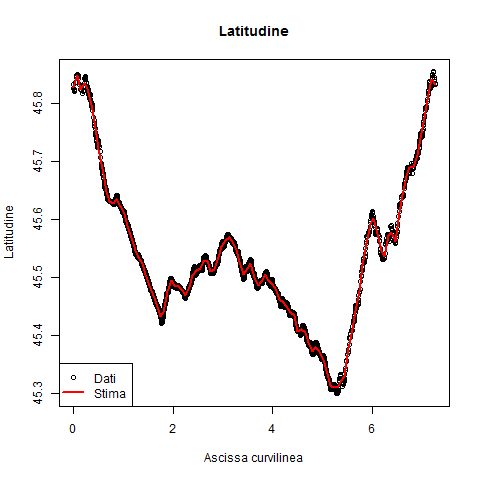
\includegraphics[width=0.50\textwidth]{Immagini/Ven_Latitudinefda.png}   
	\caption{Esempio di analisi di dati funzionali}
	\label{fig:fda}
\end{figure}

Il lavoro di tesi sarà strutturato come segue. Nel capitolo \ref{cap:panoramica} è riportato un excursus sui metodi simili già esistenti in letteratura. Nel capitolo \ref{cap:modello} è presentata la costruzione del modello matematico STR-PDE, seguita dallo sviluppo del codice R descritto nel capitolo \ref{cap:Codice}. Nel capitolo \ref{cap:domC} si hanno i primi risultati, derivanti dall'applicazione del modello e del codice R al caso del dominio a forma di C descritto in \cite{art:ramsay} e \cite{art:wood}, per il quale è possibile valutare la bontà delle stime ottenute grazie alla perfetta conoscenza del fenomeno reale in ogni punto e in ogni istante. Nel capitolo \ref{cap:confronto} il modello STR-PDE è paragonato ad altri metodi già esistenti per il confronto delle stime ottenute. Nel capitolo \ref{cap:rifiuti} si ha l'applicazione allo studio della produzione dei rifiuti nella provincia di Venezia e infine, nel capitolo \ref{cap:conclusione}, sono raccolte le conclusioni e i possibili sviluppi futuri riguardanti miglioramenti del lavoro.
\newpage
\thispagestyle{empty}




\chapter{Panoramica sui modelli già esistenti}
\label{cap:panoramica}

L'obiettivo del modello che sarà presentato in seguito è la rappresentazione funzionale di dati distribuiti in spazio e tempo. La funzione, però, non può essere identificata solo dalla minimizzazione degli scarti quadratici tra valori osservati e stimati, ma il processo di stima deve tener conto anche della regolarità della funzione. Quindi il modello STR-PDE si inserisce anche nello studio di tecniche di smoothing di dati funzionali, che prevedono la penalizzazione di opportune derivate della funzione stimata. Sono già disponibili alcune pubblicazioni riguardanti l'analisi di dati funzionali con smoothing ed è possibile evidenziare similarità o contrasti con ognuna di esse. 

Come già accennato nell'introduzione, il lavoro si propone di essere un'estensione al caso tempo-variante di quanto fatto in \cite{art:sangalli}. In questa pubblicazione si ipotizza che i dati siano distribuiti su un dominio limitato e che possano essere descritti da una funzione con l'aggiunta di rumore:
$$
z_i=f(\underline{p}_i) + \varepsilon_i \qquad \forall i \in 1\ldots n
$$
dove $\underline{p}_i$ è il vettore delle coordinate. Estendere ciò al caso tempo-variante significa aggiungere ad $f$ anche la dipendenza temporale e studiare dati che abbiano anche un'informazione legata al tempo, appartenente ad un intervallo fissato. L'approccio seguito, però, sarà differente sotto alcuni aspetti. Per poter stimare la funzione solo spaziale in \cite{art:sangalli} era posto un funzionale di penalizzazione da minimizzare con la somma di un termine di scarti quadratici tra dati e valori stimati dal modello e di un integrale del laplaciano della funzione (utile ad avere una stima più o meno liscia). Il problema di minimo era ridotto ad un problema variazionale che, per poter essere risolto computazionalmente, necessitava della riduzione di $f$ ad una combinazione lineare di funzioni di base. Quindi la possibilità di avere una soluzione era dovuta al passaggio da una formulazione complessa esatta ad una più semplice (risolvibile tramite un sistema lineare) e approssimata, vincolando l'appartenenza della funzione ad uno spazio finito-dimensionale. Nell'approccio seguito in questo lavoro, come si potrà vedere in seguito, non sarà così. Tuttavia l'articolo è stato da ispirazione per molte cose: la scelta di adottare gli elementi finiti come basi in spazio, la penalizzazione del laplaciano come misura di regolarità in spazio, l'uso di alcune matrici (come $R_0$ e $R_1$, che si ritroveranno nel prossimo capitolo nella spiegazione analitica del modello) derivano dalla volontà di estendere il caso puramente spaziale.

Anche in \cite{art:augustin} è analizzato un metodo per l'analisi di dati distribuiti in spazio e tempo. Questo lavoro, però, si basa su modelli additivi generalizzati (GAMM), costruiti per spiegare una funzione del valore atteso della risposta (nell'articolo è usato il logaritmo) tramite uno o più termini funzionali:
$$
\log(\mathbb{E}[z_i])= f_1+f_2+ \ldots +\varepsilon_i \ .
$$
Anche in \cite{art:marra} è eseguita la stessa analisi, ma con una sola funzione. La costruzione di queste pubblicazioni, quindi, è più complessa del modello STR-PDE, in cui si studia una sola funzione di risposta e non si fa uso di modelli generalizzati. Tuttavia, in \cite{art:augustin} e in \cite{art:marra} è posta un'ipotesi molto interessante: già dall'inizio la funzione è espressa come sviluppo di funzioni di base. Questo può essere considerato come il maggior punto di incontro del modello STR-PDE con GAMM, poichè non sarà creato un problema esatto da approssimare solo alla fine della costruzione del modello, ma sarà imposta già da subito una rappresentazione finito-dimensionale.


\chapter{Presentazione del modello STR-PDE}
\label{cap:modello}
In questo capitolo viene descritto nel dettaglio il modello STR-PDE per l'analisi di dati distribuiti in spazio e tempo ed è calcolata la soluzione al problema di stima.


\section{Caso senza covariate}

\subsection{Dati e modello}

Siano $\{\underline p_i = (x_i,y_i); i=1, \ldots , n\}$ un insieme di $n$ punti spaziali in un dominio limitato $\Omega \subset \mathbb R^2$ e siano $\{t_j ; j=1, \ldots , m\}$ un insieme di $m$ istanti temporali in un intervallo $[0,T]\subset \mathbb R$. In questi punti ed istanti si osservano i dati: siano quindi $\{ z_{ij};i=1, \ldots , n; j=1, \ldots , m \}$ i valori della variabile reale nel punto $\underline p_i$ al tempo $t_j$.

Sarebbe possibile trattare i dati come provenienti da funzioni tempo-varianti in ognuno dei punti spaziali considerati, cioè ipotizzare che le osservazioni $z_{ij}$ provengano da una funzione $z_i(t)$ valutata all'istante $t_j$. Questa marginalizzazione può analogamente essere eseguita in spazio, supponendo che per ogni istante di tempo esista una funzione spaziale definita su $\Omega$ che genera i dati. Tuttavia in questa analisi non si studiano modelli marginali, ma si ipotizza che le osservazioni $\{z_{ij}; i=1, \ldots , n; j=1, \ldots , m\}$ siano generate da un campo spazio-temporale con l'aggiunta di rumore:
\begin{equation}
\label{eq:modellobase}
z_{ij}=f(\underline p_i,t_j)+\varepsilon_{ij}\ \ \ \ i = 1,\ldots,n\ \ j=1,\ldots,m \ \ ,
\end{equation}
dove $\{ \varepsilon_{ij}; i = 1,\ldots ,n; j=1,\ldots m\}$ sono residui indipendenti identicamente distribuiti di media nulla e varianza $\sigma^2$. L'obiettivo del modello STR-PDE sarà la stima della funzione $f(\underline p,t)$ dalle $nm$ osservazioni a disposizione, minimizzando un funzionale $J_{\underline \lambda }(f(\underline p,t))$ con la somma degli scarti quadratici tra le osservazioni e valori stimati e termini di penalizzazione delle derivate per la regolarità della funzione.



\subsection{Definizione delle funzioni di base per $f(\protect\underline{p},t)$}
\label{subs:basi}

Dall'analisi della letteratura già disponibile per modelli simili, anche se solo spaziali, si può dedurre che non è possibile dare una stima della funzione se essa non risulta espressa in una espansione di opportune funzioni di base. Infatti l'infinita possibilità di variazione di una funzione in un qualsiasi spazio funzionale non renderebbe possibile una stima computazionale del risultato. L'approccio scelto per la costruzione di $f(\underline p,t)$ si basa sulla generalizzazione delle espansioni in funzione di base dei casi puramente spaziali o temporali.

Siano 
$$
\{ \varphi_k(t);k=1, \ldots , M \} \subset H^2([T_1,T_2])
$$
un insieme di $M$ funzioni di base definite sull'intervallo temporale $[T_1,T_2]$ e
$$
\{ \psi_l(\underline p);l=1, \ldots , N \} \subset H^1(\Omega)
$$
in insieme di $N$ funzioni di base definite sul dominio spaziale $\Omega$. Con le combinazioni lineari
$$
\sum_{k=1}^M a_k\varphi_k(t) \qquad \sum_{l=1}^N b_l\psi_l(\underline p)
$$
è possibile costruire, rispettivamente, funzioni varianti soltanto in tempo e in spazio. La funzione $f(\underline p,t)$ nasce ipotizzando che i coefficienti costanti delle espansioni in base precedenti possano variare secondo la variabile che non è espressa dalle funzioni di base:
\begin{equation} 
\label{eq:f_temp}
f(\underline p, t) = \sum_{k=1}^M a_k(\underline p)\varphi_k(t)
\end{equation}
\begin{equation}
\label{eq:f_space}
f(\underline p, t) = \sum_{l=1}^N b_l(t)\psi_l(\underline p) \ .
\end{equation}
Si ha quindi che $\{ a_k(\underline p);k=1, \ldots , M \}$ sono i coefficienti spazio-varianti dell'espansione in basi di temporali e $\{ b_l(t);l=1, \ldots , N \}$ sono i coefficienti tempo-varianti dell'espansione in basi spaziali. In questa costruzione la funzione $f(\underline p,t)$ possiede entrambe queste rappresentazioni.

Sono state ricavate due espressioni equivalenti per $f$ ma, come si potrà notare in seguito, questo è coerente (sarà ricavata un'espressione più specifica). Per il momento occorre soltanto aggiungere le seguenti condizioni (che saranno necessarie per la costruzione del funzionale di penalizzazione $J_{\underline \lambda }(f(\underline p,t))$) per i coefficienti appena introdotti:
$$
a_k(\underline p) \in H_{n_0}^2(\Omega) \qquad \forall k=1, \ldots , M
$$
e
$$
b_l(t) \in H^2([T_1,T_2]) \qquad \forall l=1, \ldots , N \ ,
$$
dove $H^2_{n_0}(\Omega) = \{h \in H^2(\Omega) | \partial _{\nu}h=0 \mbox{ su } \partial \Omega\}$, spazio incluso in $H^2(\Omega)$ che garantisce alle funzioni $a_k(\underline p)$ di avere condizioni di Neumann alla frontiera.


\subsection{Funzionale di penalizzazione $J_{\protect\underline{\lambda}}(f(\protect\underline{p},t))$}

Per poter stimare $f(\underline p,t)$ si introduce la minimizzazione di un funzionale non formato solamente dagli scarti quadratici tra le osservazioni e le stime negli $nm$ punti disponibili. Sono inclusi in esso anche altri due termini, che derivano dalla penalizzazione di opportune derivate in spazio e tempo per poter garantire regolarità alla funzione. Analogamente a quanto fatto il \ref{subs:basi}, per costruire tale funzionale si considerano inanzitutto i problemi marginali in spazio e tempo.

Per garantire una buona regolarità spaziale alla funzione è necessario penalizzare il quadrato della norma $L^2$ del laplaciano (dove per laplaciano si intenderà, da ora in avanti, rispetto alle variabili in spazio $\underline p$). La stessa scelta è stata fatta in altre pubblicazioni come \cite{art:ramsay}, \cite{art:sangalli} e \cite{art:wood}. Quindi se $g(\underline p): \Omega \mapsto \mathbb{R}$ è una funzione spazio-variante, allora si può definire la penalizzazione della regolarità in spazio tramite:
$$
J_S\left(g(\underline p)\right)=\int_{\Omega} \Bigl( \Delta  g(\underline p  ) \Bigr)^2 d \underline p \ .
$$
Analogamente in tempo si avrà la penalizzazione del quadrato della norma $L^2$ della derivata seconda. Se $h(t): [T_1,T_2] \mapsto \mathbb{R}$, allora si avrà
$$
J_T\left(h(t)\right)=\int_{T_1}^{T_2} \Bigl( \frac{\partial^2   h(t)   }{\partial t ^2} \Bigr)^2 dt\ .
$$
Grazie alle ipotesi di regolarità introdotte in sez. \ref{subs:basi} tali penalizzazioni possono essere applicate ai coefficienti degli sviluppi delle eq. \ref{eq:f_temp} e \ref{eq:f_space}. Per questo motivo si definisce:
\begin{multline*}
J_{\underline \lambda }(f(\underline p,t))=\sum_{i=1}^n \sum_{j=1}^m \bigl( z_{ij} - f(\underline p_i,t_j) \bigr)^2 \ + \\
+\lambda_S  \sum_{k=1}^M J_S\Bigl( a_k(\underline p)\Bigr) + \lambda_T \sum_{l=1}^N J_T \Bigl( b_l(t)\Bigr) \ ,
\end{multline*}
cioè
\begin{multline}
\label{eq:penalizzdisc}
J_{\underline \lambda }(f(\underline p,t))=\sum_{i=1}^n \sum_{j=1}^m \bigl( z_{ij} - f(\underline p_i,t_j) \bigr)^2 \ + \\
+\lambda_S  \sum_{k=1}^M \int_{\Omega} \Bigl( \Delta(  a_k(\underline p)  ) \Bigr)^2 d \underline p + \lambda_T \sum_{l=1}^N\int_{T_1}^{T_2} \Bigl( \frac{\partial^2   b_l(t)   }{\partial t ^2} \Bigr)^2 dt \ ,
\end{multline}
dove $\lambda_S>0$ e $\lambda_T>0$ sono i parametri di smoothing che stabiliscono il peso della penalizzazione della regolarità della funzione rispettivamente in spazio e tempo. Se troppo alti, la funzione stimata tenderà ad essere quasi liscia e distante dai dati. Al contrario, se troppo bassi, la funzione stimata sarà vicina all'interpolazione dei dati e per nulla liscia. Sebbene quest'ultimo caso possa sembrare molto buono poiché vicino ai valori osservati, non è ciò che si desidera, poiché crea una stima troppo dipendente dai dati e spesso con variazioni eccessivamente repentine. Un corretto bilanciamento di questi casi garantisce una buona descrizione del fenomeno.



\subsection{Modello ideale}
Il funzionale di penalizzazione riportato in eq. \ref{eq:penalizzdisc} è il risultato di una costruzione derivante dalle penalizzazioni marginali in spazio e tempo, ma idealmente si può ricondurre al seguente:
\begin{multline}
\label{eq:Jfunc_cont}
\tilde J_{\underline \lambda }(f) = \sum_{i=1}^n \sum_{j=1}^m \bigl( z_{ij} - f(\underline p_i,t_j) \bigr)^2 \ + \\+\   \lambda_S \int_{T_1}^{T_2} \int_\Omega \Bigl( \Delta f(\underline p, t)  \Bigr)^2 d\underline p\ dt \ +\  \lambda_T \int_\Omega \int_{T_1}^{T_2} \Bigl( \frac{\partial^2 f(\underline p, t) }{\partial t ^2} \Bigr)^2 dt\ d\underline p ,
\end{multline}
dove $J_S$ e $J_T$ sono applicati direttamente alla funzione $f(\underline p, t)$ e sono integrati, rispettivamente, sull'intervallo spaziale e il dominio spaziale. Se si applica la forma di $f(\underline p,t)$ dell'eq. \ref{eq:f_temp} nel termine di penalizzazione del laplaciano in spazio, allora si può ritrovare:
\begin{equation} 
\label{eq:espansione_funzinf_t}
\begin{split}
\int_{T_1}^{T_2} \int_\Omega \Bigl( \Delta f(\underline p, t)  \Bigr)^2 d\underline p\ dt 
&=\int_{T_1}^{T_2} \int_\Omega \Bigl( \Delta \bigl( \sum_{k=1}^M a_k(\underline p) \varphi_k(t) \bigr)  \Bigr)^2 d\underline p\ dt \\
&=\int_{T_1}^{T_2} \int_\Omega \Bigl( \sum_{k=1}^M \Delta a_k(\underline p) \varphi_k(t)  \Bigr)^2 d\underline p\ dt \\
&=\int_{T_1}^{T_2} \int_\Omega \Bigl( \sum_{k=1}^M \Delta a_k(\underline p) \varphi_k(t)  \Bigr)\Bigl( \sum_{h=1}^M \Delta a_h(\underline p) \varphi_h(t)  \Bigr) d\underline p\ dt \\
&=\int_{T_1}^{T_2} \int_\Omega \Bigl( \sum_{k=1}^M \sum_{h=1}^M \Delta a_k(\underline p)\Delta a_h(\underline p)\ \varphi_k(t)  \varphi_h(t)  \Bigr) d\underline p\ dt \\
&=\sum_{k=1}^M \sum_{h=1}^M \int_\Omega   \Delta a_k(\underline p) \Delta a_h(\underline p)d\underline p \ \int_{T_1}^{T_2} \varphi_k(t)\varphi_h(t)   \ dt .
\end{split}
\end{equation}
Questo termine è equivalente a quello proposto in \ref{eq:penalizzdisc} se le basi temporali siano ortonormali, poichè in tal caso l'ultimo integrale in eq. \ref{eq:espansione_funzinf_t} sarebbe 1 se $k=h$ e 0 altrimenti.

Allo stesso modo, se si sostituisce la forma di $f(\underline p,t)$ dell'eq. \ref{eq:f_space} nella penalizzazione ideale dell'eq. \ref{eq:Jfunc_cont} si ottiene:
\begin{equation} 
\label{eq:espansione_funzinf_sp}
\begin{split}
\int_\Omega \int_{T_1}^{T_2} \Bigl( \frac{\partial^2 f(\underline p, t) }{\partial t ^2} \Bigr)^2 dt\ d\underline p 
&=\int_\Omega \int_{T_1}^{T_2} \Bigl( \frac{\partial^2 \sum_{l=1}^N b_l(t)\psi_l(\underline p) }{\partial t ^2} \Bigr)^2 dt\ d\underline p \\
&=\int_\Omega \int_{T_1}^{T_2} \Bigl( \sum_{l=1}^N \frac{ \partial^2b_l(t)}{\partial t ^2}\psi_l(\underline p)  \Bigr)^2 dt\ d\underline p  \\
&=\int_\Omega \int_{T_1}^{T_2} \Bigl( \sum_{l=1}^N \frac{ \partial^2b_l(t)}{\partial t ^2}\psi_l(\underline p)  \Bigr)\Bigl( \sum_{h=1}^N \frac{ \partial^2b_h(t)}{\partial t ^2}\psi_h(\underline p)  \Bigr) dt\ d\underline p \\
&= \int_\Omega \int_{T_1}^{T_2} \Bigl( \sum_{l=1}^N \sum_{h=1}^N \frac{ \partial^2b_l(t)}{\partial t ^2}\frac{ \partial^2b_h(t)}{\partial t ^2}\   \psi_l(\underline p)  \psi_h(\underline p)  \Bigr) dt\ d\underline p \\
&=\sum_{l=1}^N \sum_{h=1}^N  \int_{T_1}^{T_2}  \frac{ \partial^2b_l(t)}{\partial t ^2}\frac{ \partial^2b_h(t)}{\partial t ^2}dt\  \int_\Omega \psi_l(\underline p)  \psi_h(\underline p)    d\underline p .
\end{split}
\end{equation}
La stessa osservazione del caso precedente vale anche ora: se le basi in spazio sono ortonormali, si ritrova la penalizzazione proposta in \ref{eq:penalizzdisc}. 

In questo lavoro di tesi, quindi, è proposto un modello che risulterà essere computazionalmente semplice ma non perfettamente equivalente a questo modello ideale. In generale, le funzioni di base non sono ortonormali. Comunque sia, gli insiemi di basi che saranno adattati sono sparsi, cioè i termini $ \int_{T_1}^{T_2} \varphi_k(t)\varphi_l(t)\ dt $ e $\int_\Omega \psi_l(\underline p)  \psi_k(\underline p)d\underline p$ sono diversi da zero solo per poche coppie di indici.






\subsection{Discretizzazione dei termini di penalizzazione delle derivate}
Così come è scritto in \ref{eq:penalizzdisc}, il funzionale $J_{\underline \lambda }(f(\underline{p},t))$ non è ancora adatto ad essere trattato computazionalmente. Per poter avere una forma che renda semplice la stima, $f(\underline{p},t)$ e $J_{\underline \lambda }(f(\underline{p},t))$ saranno nuovamente discretizzati. 

Il primo caso da trattare è l'integrale del laplaciano dei coefficienti spazio-varianti dell'eq. \ref{eq:f_temp} in modo analogo a quanto fatto in \cite{art:sangalli}. Fissato $k$, l'integrale
$$
\int_{\Omega} \Bigl( \Delta(  a_k(\underline p)  ) \Bigr)^2 d \underline p
$$
può essere semplificato introducendo la funzione $g_k(\underline p) \in L^2(\Omega)$ come segue:
\begin{equation}
\label{eq:ps1}
\int_\Omega g_k(\underline{p}) v(\underline{p}) d \Omega= \int_\Omega \Delta (a_k(\underline p)) v(\underline p) d \Omega\qquad \forall v(\underline{p}) \in L^2(\Omega) \ .
\end{equation}
Non è difficile verificare che, se $g_k(\underline p)$ rispetta l'equazione precedente, per l'arbitrarietà di $v$ allora:
\begin{equation}
\label{eq:ps2}
\int_{\Omega} \Bigl( \Delta(  a_k(\underline p)  ) \Bigr)^2 d \underline p = \int_{\Omega}  \Delta(  a_k(\underline p))g_k(\underline p)d \underline p \ .
\end{equation}
Applicando la la formula di Green e tenendo conto delle condizioni di Neumann per $a_k(\underline p)$, si possono semplificare gli integrali eliminando l'uso del laplaciano:
$$
\int_{\Omega}  \Delta(  a_k(\underline p))g_k(\underline p)d \underline p \ = -\int_{\Omega} \nabla  a_k(\underline p)\nabla g_k(\underline p)d \underline p
$$
$$
\int_{\Omega}  \Delta(  a_k(\underline p))v(\underline p)d \underline p \ = -\int_{\Omega} \nabla  a_k(\underline p)\nabla v(\underline p)d \underline p \ .
$$
Per poter calcolare analiticamente questi integrali è necessario introdurre l'uso delle basi spaziali $\{ \psi_l(\underline p);l=1, \ldots , N \}$ per le funzioni $a_k$, $g_k$ e $v$. Siano quindi:
$$
a_k(\underline p)=\sum_{l=1}^N c_{lk}\psi_l(\underline p) \qquad 
g_k(\underline p)=\sum_{l=1}^N g_{lk}\psi_l(\underline p) \qquad
v(\underline p)=\sum_{l=1}^N v_{l}\psi_l(\underline p) \ .
$$
Per semplificare le notazioni saranno usati i seguenti vettori:
$$
\underline c_k =
\begin{bmatrix}
c_{1k} \\ c_{2k} \\ \hdots \\ c_{Nk}
\end{bmatrix}
\qquad
\underline g_k =
\begin{bmatrix}
g_{1k} \\ g_{2k} \\ \hdots \\ g_{Nk}
\end{bmatrix}
\qquad
\underline v =
\begin{bmatrix}
v_1 \\ v_2 \\ \hdots \\ v_N
\end{bmatrix} 
$$
e gli analoghi per le funzioni di base e le loro derivate parziali:
$$
\underline \psi =
\begin{bmatrix}
\psi_{1}  \\
\psi_{2}  \\
\vdots\\
\psi_{N}
\end{bmatrix}
$$
\begin{equation}
\underline \psi_x=  \begin{bmatrix}
\partial \psi_{1}/\partial x \\
\partial \psi_{2}/\partial x  \\
\vdots\\
\partial \psi_{N}/\partial x \end{bmatrix} 
\qquad
\underline \psi_x=  \begin{bmatrix}
\partial \psi_{1}/\partial y  \\
\partial \psi_{2}/\partial y  \\
\vdots\\
\partial \psi_{N}/\partial y\end{bmatrix} \ .
\end{equation}
Mediante l'uso delle funzioni di base e di ciò che è stato ottenuto dall'applicazione della formula di Green, le relazioni \ref{eq:ps1} e \ref{eq:ps2} diventano:
$$
\underline{g}_k \Bigl(\int_\Omega \underline \psi \underline \psi^T \Bigr)\underline{v}=
-\underline{c}_k \Bigl(\int_\Omega (\underline \psi_x \underline \psi_x^T + \underline \psi_y \underline \psi_y^T)\Bigr) \underline{v} \qquad \forall \underline{v} \in \mathbb{R}^N
$$
$$
\int_{\Omega} \Bigl( \Delta(  a_k(\underline p)  ) \Bigr)^2 d \underline p = -\underline{c}_k \Bigl(\int_\Omega (\underline \psi_x \underline \psi_x^T + \underline \psi_y \underline \psi_y^T) \Bigr)\underline{g}_k \ .
$$
Quindi, se si introducono le matrici (analogamente a quanto fatto in \cite{art:sangalli})
$$ R_0 = \int_\Omega \underline \psi \underline \psi^T $$
$$ R_1 = \int_\Omega (\underline \psi_x \underline \psi_x^T + \underline \psi_y \underline \psi_y^T) \ ,$$
si trova, per l'arbitrarietà di $\underline v$:
\begin{equation}
\label{eq:pspace}
\int_{\Omega} \Bigl( \Delta(  a_k(\underline p)  ) \Bigr)^2 d \underline p = \underline{c}_k^T R_1 R_0^{-1} R_1 \underline{c}_k=\underline{c}_k^T P_S \underline{c}_k
\end{equation}
Si noti che la matrice $P_S$ non dipende da $k$ e può essere considerata la stessa per tutte le funzioni $a_k(\underline{p})$. Inoltre è simmetrica, poichè $R_0$ e $R_1$ lo sono.

Grazie all'introduzione della discretizzazione in basi spaziali
$$
a_k(\underline p)=\sum_{l=1}^N c_{lk}\psi_l(\underline p)
$$
è stato possibile ridurre la penalizzazione con l'integrale del quadrato di $\Delta a_k(\underline p)$
alla valutazione di una forma quadratica che non cambia con le funzioni $a_k$. Si ha anche un'altra conseguenza: per l'equivalenza ipotizzata tra le espressioni di $f(\underline{p},t)$ in \ref{eq:f_temp} e \ref{eq:f_space}, allora è necessario che i coefficienti tempo-varianti dell'espansione in basi spaziali assumano la seguente forma:
$$
b_l(t)=\sum_{k=1}^M c_{lk}\varphi_k(t) \ .
$$
Si ritrova quindi anche in questo caso l'espansione in funzioni di base.

Non resta altro che discretizzare anche $\int_{T_1}^{T_2} \Bigl( \frac{\partial^2   b_l(t)   }{\partial t ^2} \Bigr)^2 dt$. Dopo aver introdotto l'uso delle funzioni di base, se si definisce 
 $$ P_T = \begin{bmatrix}
\int_{T_1}^{T_2} \varphi_1''(t) \varphi_1''(t) dt  & \int_{T_1}^{T_2} \varphi_1''(t) \varphi_2''(t) dt & \hdots & \int_{T_1}^{T_2} \varphi_1''(t) \varphi_M''(t) dt  \\
\int_{T_1}^{T_2} \varphi_2''(t) \varphi_1''(t) dt  & \int_{T_1}^{T_2} \varphi_2''(t) \varphi_2''(t) dt & \hdots & \int_{T_1}^{T_2} \varphi_2''(t) \varphi_M''(t) dt  \\
\vdots & \vdots & \hdots & \vdots \\
\int_{T_1}^{T_2} \varphi_M''(t) \varphi_1''(t) dt  & \int_{T_1}^{T_2} \varphi_M''(t) \varphi_2''(t) dt & \hdots & \int_{T_1}^{T_2} \varphi_M''(t) \varphi_M''(t) dt  \\
\end{bmatrix} $$
e il vettore $$
\underline{c}_l =
\begin{bmatrix}
c_{l1} \\ c_{l2} \\ \hdots \\ c_{lM}
\end{bmatrix} \ ,$$ si ritrova:
$$
\int_{T_1}^{T_2} \Bigl( \frac{\partial^2   b_l(t)   }{\partial t ^2} \Bigr)^2 dt = \underline{c}_l^T  P_T \underline{c}_l \ .
$$
Anche la matrice $P_T$ è simmetrica.

L'introduzione di $P_S$ e $P_T$ può essere ulteriormente sviluppata per dimostrare che la parte di penalizzazione per la regolarizzazione di $f$ in \ref{eq:penalizzdisc} sia rappresentabile con un'unica forma quadratica. Per mostrarlo, si introduce il vettore
$$\underline c =
\begin{bmatrix}
c_{11}  \\
\vdots\\
c_{1M}  \\
c_{21}  \\
\vdots\\
c_{2M}  \\
\vdots\\
c_{NM}
\end{bmatrix}
$$
e la matrice $P$, definita con opportuni prodotti di Kronecker come segue:
$$
P = \lambda_S\    (P_S \otimes I_M)   \ +\  \lambda_T\   (I_N \otimes P_T) \ ,
$$
dove $I_M$ and $I_N$ sono matrici identità di dimensioni $M \times M$ e $N \times N$ rispettivamente. Allora si avrà:
\begin{multline}
\lambda_S  \sum_{k=1}^M \int_{\Omega} \Bigl( \Delta(  a_k(\underline p)  ) \Bigr)^2 d \underline p + \lambda_T \sum_{l=1}^N\int_{T_1}^{T_2} \Bigl( \frac{\partial^2   b_l(t)   }{\partial t ^2} \Bigr)^2 dt =
\\ = \lambda_S\sum_{k=1}^M\underline{c}_k^T P_S \underline{c}_k + \lambda_T\sum_{l=1}^N\underline{c}_l^T P_T \underline{c}_l = \underline{c}^T P \underline{c} \ .
\end{multline}
A causa della simmetria dei termini con cui è costruita, anche la matrice $P$ è simmetrica.


\subsection{Soluzione del problema di stima}
Grazie a quanto ricavato nel paragrafo precedente, la parte di penalizzazione delle derivate del funzionale $J_{\underline \lambda }(f(\underline p,t))$ si è ridotta ad un'unica forma quadratica. Ma questo è stato possibile grazie all'espressione in funzione di base per i coefficienti delle eq. \ref{eq:f_temp} e \ref{eq:f_space}:
$$
a_k(\underline p)=\sum_{l=1}^N c_{lk}\psi_l(\underline p) \qquad b_l(t)=\sum_{k=1}^M c_{lk}\varphi_k(t) \ .
$$
Essendo \ref{eq:f_temp} e \ref{eq:f_space} equivalenti, allora in definitiva:
\begin{equation} 
\label{eq:basisexp}
f(\underline p,t)=\sum_{l=1}^N \sum_{k=1}^M c_{lk}\ \psi_l(\underline p)\ \varphi_k(t) ,
\end{equation}
cioè la funzione da stimare è la combinazione lineare di tutti i possibili prodotti incrociati tra le funzioni di base in tempo e spazio. Questa formulazione può essere considerata la definitiva per la funzione $f(\underline p,t)$ e permette di poter identificare la funzione con il vettore dei suoi coefficienti $\underline{c}$. Ne consegue anche la possibilità di scrivere in modo più agevole il funzionale $J_{\underline \lambda }(f(\underline p,t))$. Siano definiti il vettore dei valori osservati
\begin{equation}
\underline z =
\begin{bmatrix}
z_{11}  \\
\vdots\\
z_{1m}  \\
z_{21}  \\
\vdots\\
z_{2m}  \\
\vdots\\
z_{nm}
\end{bmatrix}
\end{equation}
e le matrici $\Psi$ (con le valutazioni delle basi spaziali nei punti $\{\underline p_i; i = 1,\ldots,n\}$) e $\Phi$ (con le valutazioni delle basi temporali $\{t_j; j = 1,\ldots,m\}$):
$$
\Psi =
\begin{bmatrix}
\psi_{1}(\underline p_1) & \psi_{2}(\underline p_1) & \hdots & \psi_{N}(\underline p_1)  \\
\psi_{1}(\underline p_2) & \psi_{2}(\underline p_2) & \hdots & \psi_{N}(\underline p_2)  \\
\vdots & \vdots & \hdots & \vdots \\
\psi_{1}(\underline p_n) & \psi_{2}(\underline p_n) & \hdots & \psi_{N}(\underline p_n)  \\
\end{bmatrix}
$$
$$
\Phi = 
\begin{bmatrix}
\varphi_{1}( t_1) & \varphi_{2}( t_1) & \hdots & \varphi_{M}( t_1)  \\
\varphi_{1}( t_2) & \varphi_{2}( t_2) & \hdots & \varphi_{M}( t_2)  \\
\vdots & \vdots & \hdots & \vdots \\
\varphi_{1}( t_m) & \varphi_{2}( t_m) & \hdots & \varphi_{M}( t_m)  \\
\end{bmatrix} \ .
$$
Le ultime due matrici non sono utili da sole, ma moltiplicate tra loro con prodotto di Kronecker, poichè se
$$ B = \Psi \otimes \Phi \ ,$$
allora si può facilmente dire che:
$$
\begin{bmatrix}
f(\underline p_1,t_1)  \\
\vdots\\
f(\underline p_1,t_m)  \\
f(\underline p_2,t_1)  \\
\vdots\\
f(\underline p_2,t_m)  \\
\vdots\\
f(\underline p_n,t_m)
\end{bmatrix}= B \underline c \ .
$$
Quindi è possibile dare una forma definitiva al funzionale di penalizzazione:
\begin{equation} 
\label{eq:Jmatr}
J_{\underline \lambda }(\underline c) = (\underline z - B \underline c)^T (\underline z - B \underline c) + \underline c^T P \underline c \ ,
\end{equation}
e per trovare la stima della funzione $f(\underline{p},t)$ sarà sufficiente ricavare il vettore dei coefficienti $\underline c$ risolvendo il problema di minimo:
$$
\hat{\underline{c}}=\argmin_{c \in \mathbb{R}^{NM}} J_{\underline \lambda }(\underline c) \ .
$$
Mediante la formulazione ottenuta in \ref{eq:Jmatr} basta derivare per ottenere la soluzione al problema di stima. Grazie alla simmetria di $P$, si ha:
$$
\frac{\partial}{\partial \underline c}J= -2 B^T \underline z + 2(B^T B + P) \underline c \ \ ,
$$
che posta uguale a zero porta all'equazione
$$
(B^T B + P) \underline c = B^T\underline z
$$ 
e in conclusione
\begin{equation}
\label{eq:sysnocovar}
\hat  {\underline c} = (B^T B + P)^{-1}B^T \underline z \ .
\end{equation} 

Il problema di stima è stato risolto e la soluzione si può trovare risolvendo un sistema lineare, seppur di grandi dimensioni (la matrice $B^T B + P$ ha dimensioni $NM \times NM$ e già negli esempi si avranno dimensioni elevate).

L'ultimo elemento da definire è la \textit{smoothing matrix} $S$, che permette di derivare i valori stimati dal modello direttamente da quelli osservati:
$$
\hat  {\underline z} =B\hat  {\underline c} = B(B^T B + P)^{-1}B^T \underline z = S\underline{z} \ .
$$



\subsection{Proprietà statistiche di $\hat  {\protect\underline{c}}$}
Il modello di partenza indicato in \ref{eq:modellobase} può essere scritto anche in forma matriciale
\begin{equation}
\label{eq:modellobasematric}
\underline z=B \underline c + \underline \varepsilon .
\end{equation}
A causa delle proprietà statistiche di $\underline \varepsilon$
$$
\mathbb{E}[\underline \varepsilon] = \underline 0 \qquad \mathrm{Var}[\underline \varepsilon] = \sigma^2 I_{nm}
$$
si ha
$$
\mathbb{E}[\underline z] = B \underline c \qquad \mathrm{Var}[\underline z] = \sigma^2 I_{nm}
$$
e quindi è immediato ricavare per lo stimatore $\hat  {\underline c}$ (grazie alle proprietà simmetria di $P$):
$$
\mathbb{E}[\hat  {\underline c}] = (B^T B + P)^{-1}B^TB \underline c \qquad \mathrm{Var}[\hat  {\underline c}] = \sigma^2 (B^T B + P)^{-1}B^TB(B^T B + P)^{-1} .
$$
Non è stata ipotizzata la gaussianità per $\underline \varepsilon$, ma se così fosse anche $\hat  {\underline c}$ sarebbe gaussiano. Attraverso questa ulteriore ipotesi sarebbe possibile elaborare (con una data significatività) una regione di confidenza per $\hat  {\underline c}$ e quindi una banda di confidenza per la funzione stimata $f$.


\section{Caso con covariate}
\label{sez:beta}
Il modello si estende facilmente se si prevede che il dato possa essere influenzato da covariate. La forma in eq. \ref{eq:modellobase} diventa:
\begin{equation}
\label{eq:modellobasecovar}
z_{ij}= \underline w_{ij}^T\  \underline \beta   \ + \  f(\underline p_i,t_j)\ +\ \varepsilon_{ij}\ \ \ \ i = 1,\ldots,n\ \ j=1,\ldots,m \ \ ,
\end{equation}
dove $\underline w_{ij}$ è il vettore delle $p$ covariate associate a $z_{ij}$ e $\underline \beta$ è il vettore dei coefficienti di regressione. Di conseguenza il funzionale discreto di \ref{eq:Jmatr} diventa:
$$ J_{\underline \lambda }(\underline c) = (\underline z - W \underline \beta - B \underline c)^T (\underline z - W \underline \beta - B \underline c) + \underline c^t S \underline c  \ ,$$
dove $W$ è la matrice $nm \times p$ con i vettori $ \{\underline w_{ij}; i=1,\ldots,n;j=1,\ldots,m\}$.

Per trovare la soluzione occorre derivare questa espressione rispetto a $\underline \beta$ e $\underline c$:
$$
\frac{\partial}{\partial \underline \beta}J= -2W^T \underline z + 2W^T B \underline c + 2 W^TW \underline \beta \ \ ,
$$
$$
\frac{\partial}{\partial \underline c}J= -2 B^T \underline z + 2 B^T W \underline \beta + 2(B^T B + P) \underline c \ \ .
$$
Imponendo che le derivate siano uguali a zero si ha:
$$
\begin{cases}
W^TW \hat{\underline \beta} = W^T(\underline z - B \hat{\underline c})  \\
(B^T B + P) \hat{\underline c}=B^T(\underline z -W \hat{\underline \beta})
\end{cases}.
$$
Queste due equazioni ricordano quelle usate per la regressione lineare e per il modello senza covariate, con la differenza che in questo caso a $\underline z$ è sottratta, in entrambi i casi, la parte spiegata dal termine di modello a cui non si riferiscono $\hat{\underline \beta}$ e $\hat{\underline c}$ rispettivamente.

A questo punto si possono ricavare le stime dei parametri. Per i coefficienti della funzione si trova:

\begin{eqnarray}
 \label{eq:syscovar1}
\hat  {\underline c} &=& [B^TB+P+B^TW(W^TW)^{-1}W^TB]^{-1}B^T[I-W(W^TW)^{-1}W^T]\underline z  \nonumber \\
 &=& AQ \underline z
\end{eqnarray} 
con $A=[B^TB+P+B^TW(W^TW)^{-1}W^TB]^{-1}B^T$ e $Q=[I-W(W^TW)^{-1}W^T]$, matrice molto importante nel caso di regressione lineare, poiché essa proietta il vettore dei dati nel sottospazio ortogonale allo spazio generato dalle colonne della matrice disegno, ricavando così il vettore dei residui. Questa matrice si ritrova anche in questo caso e sono valide le sue proprietà:
\begin{itemize}
\item $Q$ è idempotente, cioè $QQ=Q$;
\item $Q$ è simmetrica;
\item a causa del fatto che proietta nel sottospazio ortogonale di $\mathrm{Col}(W)$, $QW$ risulta essere la matrice nulla di opportune dimensioni. 
\end{itemize}
Infine, la stima di $\hat  {\underline \beta}$ si ottiene dalla stima ottenuta per $\hat  {\underline c}$:
\begin{equation}
\label{eq:syscovar2}
\hat{\underline{\beta}}=(W^TW)^{-1}W^T(I-B AQ)\underline z
\end{equation}

In modo analogo al caso senza covariate, è necessario ricavare la \textit{smoothing matrix}, poiché sarà utile in seguito:
$$
\hat  {\underline z} =B\hat  {\underline c} + W \hat  {\underline \beta} = [B AQ + W(W^TW)^{-1}W^T(I-B AQ)]\underline z = S\underline z .
$$

\subsection{Proprietà statistiche di $\hat  {\protect\underline{c}}$ e $\hat  {\protect\underline{\beta}}$}
\label{sec:IC}
Anche in questo caso è possibile calcolare valore atteso e varianza degli stimatori ottenuti. Questo è particolarmente utile in presenza di covariate, poichè consente di calcolare intervalli di confidenza o effettuare test per verificarne la sisignificatività. Per farlo, però, è necessario avere la forma matriciale del modello indicato in \ref{eq:modellobasecovar}:

\begin{equation}
\label{eq:modellobasecovarmatric}
\underline z=B \underline c + W \underline \beta + \underline \varepsilon .
\end{equation}
Di nuovo si ha 
$$
\mathbb{E}[\underline \varepsilon] = \underline 0 \qquad \mathrm{Var}[\underline \varepsilon] = \sigma^2 I_{nm}
$$
e di conseguenza
$$
\mathbb{E}[\underline z] = B \underline c + W \underline \beta \qquad \mathrm{Var}[\underline z] = \sigma^2 I_{nm} .
$$
Mediate questo risultato e le proprietà ricavate per la matrice $Q$ è possibile ottenere che:
$$
\mathbb{E}[\hat  {\underline c}] = AQB \underline c \qquad \mathrm{Var}[\hat  {\underline c}] = \sigma^2 AQA^T .
$$
Per $\hat  {\underline \beta}$ i calcoli sono più complessi, ma si semplificano grazie alle proprietà indicate in precedenza per la matrice $Q$. Si ritrova:
$$
\mathbb{E}[\hat  {\underline \beta}] = \underline \beta + (W^TW)^{-1}W^T(I-B AB)\underline c
$$
$$ \mathrm{Var}[\hat  {\underline \beta}] = \sigma^2 (W^TW)^{-1} + \sigma^2 (W^TW)^{-1}W^T B A Q A^T B^T W(W^TW)^{-1}.
$$
Come nel caso senza covariate, anche ora si avrebbe la gaussianità degli stimatori se fosse ipotizzata per $\underline \varepsilon$. Se questa ipotesi fosse posta sarebbe possibile elaborare intervalli di confidenza o test per le componenti di $\underline \beta$ e verificarne la significatività. Tuttavia si può notare un termine di distorsione in $\mathbb{E}[\hat  {\underline \beta}]$ che complica l'inferenza su $\underline \beta$. Quindi nel codice R è stato deciso di non considerare tale distorsione, per avere intervalli di confidenza simmetrici e per non complicare eccessivamente questi calcoli. 


\section{Stima di $\sigma^2$ e scelta dei parametri $\lambda_S$ e $\lambda_T$}
\label{sez:GCV}

Quanto riportato di seguito è valido indipendentemente dal fatto che siano inserite nel modello le covariate, quindi per entrambi i modelli proposti in precedenza.

\subsection{Stima di $\sigma^2$}
Stimare la varianza dell'errore è necessario se si vuole fare inferenza sugli stimatori ed è molto semplice se si conoscono i gradi di libertà equivalenti del modello. Ma questi si ricavano dalla \textit{smoothing matrix}:
$$
\mathrm{EDF}=\mathrm{tr}(S) \ .
$$
Con questo valore si calcola la stima della varianza, usando i residui e il numero totale di dati:
$$
\hat{\sigma}^2=\frac{1}{nm-tr(S)}(\underline z - \hat  {\underline z})^T(\underline z - \hat  {\underline z})
$$

\subsection{Parametri $\lambda_S$ e $\lambda_T$}
I parametri $\lambda_S$ e $\lambda_T$ hanno un ruolo rilevante nella stima della soluzione, poichè scelgono quanto peso dare alla regolarità della funzione in spazio e tempo. Quindi è opportuno che siano fissati accuratamente prima della stima della soluzione.

Secondo quanto indicato in \cite{art:marra}, la scelta corretta si ha con il valore di $\underline \lambda$ che realizza il minimo dell'indice di \textit{generalized cross validation}
$$
\mathrm{GCV}(\underline \lambda) =\frac{nm}{nm-\text{tr}(S)}  D(\hat  {\underline c},\hat  {\underline \beta}) \ ,
$$
dove $D$ è la devianza del modello. Essa è così definita:
$$
D(\hat  {\underline c},\hat  {\underline \beta})=2\sigma^2(l_{\mathrm{sat}}-l(\hat  {\underline c},\hat  {\underline \beta})) \ ,
$$
dove $l$ è la logverosimiglianza del modello, che si ipotizza gaussiano, valutata rispettivamente nel suo massimo (valore di saturazione) e in corrispondenza dei valori stimati. Non è difficile dimostrare che, sia nel caso con covariate che senza covariate, si ha: 
$$
D(\hat  {\underline c},\hat  {\underline \beta}) = (\underline z - \hat  {\underline z})^T(\underline z - \hat  {\underline z})
$$
Di conseguenza, il miglior $\underline \lambda$ può essere scelto come valore che minimizza
\begin{equation}
\label{eq:GCV}
\mathrm{GCV}(\underline \lambda) =\frac{nm}{nm-\text{tr}(S)}  (\underline z - \hat  {\underline z})^T(\underline z - \hat  {\underline z}) \ .
\end{equation}

\chapter{Sviluppo del codice R}
\label{cap:Codice}
Il modello descritto nel capitolo precedente è stato associato ad un algoritmo e ha portato allo sviluppo di un codice R per l'analisi dei dati. In questo capitolo saranno spiegate alcune delle scelte adottate o imposte durante la fase di sviluppo computazionale.

Il linguaggio di programmazione adottato è R. Questa decisione ha permesso di sfruttare le numerose funzioni statistiche che in altri linguaggi non sarebbero disponibili. Ma, come si potrà notare in seguito, sono anche emersi i lati negativi di questo linguaggio. Durante l'implementazione si è fatto uso del pacchetto \textit{fda} e di alcune funzioni già disponibili per il caso puramente spaziale descritto in \cite{art:sangalli}.

\section{Funzioni di base disponibili nel codice}
Sono stati implementati solo alcuni tipi di funzione di base in spazio e tempo, che si sono rivelate utili alle applicazioni che saranno riportate nei capitoli successivi. 

Per quanto riguarda lo spazio, il codice è stato pensato per dati distribuiti su un dominio bidimensionale anche complesso (con bordi irregolari o buchi). Quindi un'ottima scelta di funzioni di base sono gli elementi finiti descritti in REFERENZA NECESSARIA. Queste funzioni sono costruite su una triangolazione del dominio, definita dai vertici del poligono che descrive la frontiera e dai punti interni (solitamente quelli in cui sono disponibili i dati). Ognuno di questi punti diventa un nodo della triangolazione e ad ogni nodo è associata una funzione lineare a tratti come quella in \ref{fig:basisp}, che vale 1 sul nodo selezionato, decresce linearmente sui triangoli adiacenti e si annulla su tutti gli altri nodi e triangoli. Per l'implementazione di queste funzioni è stato riutilizzata una parte del codice del caso puramente spaziale. Anche gli elementi finiti quadratici sono stati implementati, ma non sono stati scelti nelle applicazioni poiché rallentano l'esecuzione a causa della maggiore precisione che richiedono.

\begin{figure}[t]
	\centering
	\subfigure[Elemento finito (spazio)]
	{
	\label{fig:basisp}
	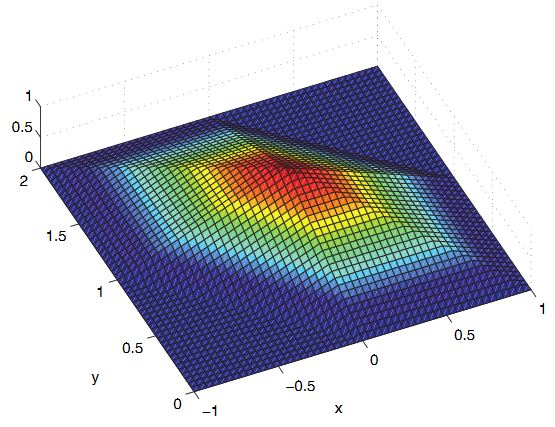
\includegraphics[width=0.46\textwidth]{Immagini/elementofinito.jpg}  
   }
	\subfigure[B-splines (tempo)]
   {
   \label{fig:basit}
	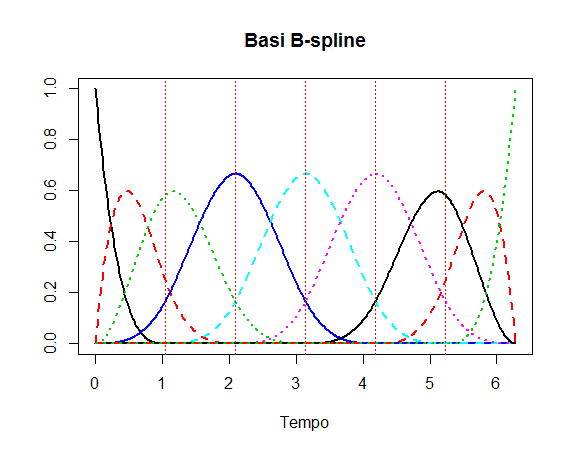
\includegraphics[width=0.46\textwidth]{Immagini/Bsplines.png}
   }
	\caption{Funzioni di base implementate nel codice}
	\label{fig:basi}
\end{figure}

Le basi in tempo a disposizione sono le B-splines, funzioni che, fissato un intervallo temporale e alcuni nodi in esso contenuti (nel nostro caso equispaziati), sono usate per l'espansione in base delle \textit{funzioni spline}. Il codice necessario è già stato implementato ed ottimizzato nel pacchetto \textit{fda} ed è stato riciclato per il codice del modello STR-PDE. In fig. \ref{fig:basit} sono riportate le 9 B-splines cubiche definite sull'intervallo $[0,2\pi]$ (che sarà usato per l'applicazione al dominio a forma di C). L'unico vincolo imposto a queste funzioni di base è il grado, che deve essere almeno 3 per avere la derivata seconda delle basi necessaria per la penalizzazione.

\section{Schematizzazione dell'algoritmo di stima}
L'esecuzione del codice è stata divisa in alcuni passi per poter permettere all'utente di inserire gradualmente gli oggetti in ingresso e fissare i parametri che servono per ottenere la stima finale. In più punti si è cercato di nascondere all'utente le variabili temporanee e di includere in opportune classi di R tutte le informazioni riguardanti concetti tra di loro comuni. 

Inanzitutto si ha l'acquisizione dei dati (e delle eventuali covariate) e la creazione della triangolazione. In questo caso non sono state implementate funzioni apposite poiché ci sono già pacchetti specializzati (nelle applicazioni che saranno presentate in seguito si è fatto uso di \textit{RTriangle} per la triangolazione).

Dopo aver definito i punti, la triangolazione e gli istanti di tempo occorre fissare le funzioni di base. Sono state implementate due funzioni di R, una per lo spazio e una per il tempo, che in base ai parametri in ingresso e agli ordini scelti per le funzioni di base creano appositi oggetti che memorizzano tutte le informazioni necessarie.  

A questo punto si ha la ricerca i migliori parametri di smoothing: definiti un insieme discreto di valori per $\lambda_S$ ed uno analogo su $\lambda_T$, l'indice in eq. \ref{eq:GCV} è minimizzato sul prodotto cartesiano di tali insiemi. Per una corretta applicazione del modello questa operazione deve essere ripetuta più volte, fino al raggiungimento di una accettabile precisione nella stima di $\underline{\lambda}$. Sono state implementate due funzioni, una per il caso senza covariate e una per il caso con covariate, a causa della diversità della \textit{smoothing matrix}. Questo è il passaggio più lento dell'algoritmo.

Dopo aver fissato i parametri di smoothing si arriva al cuore dell'algoritmo, poiché è calcolata la stima della soluzione. Ciò che eseguono le apposite funzioni è calcolare tutte le matrici di passaggio ($P$ e $B$) nascondendole all'utente e risolvere gli appositi sistemi lineari (eq. \ref{eq:sysnocovar}, \ref{eq:syscovar1} e \ref{eq:syscovar2}). In uscita è restituito un oggetto che racchiude i vettori ricavati e le funzioni di base, in modo da poter immagazzinare insieme tutti gli elementi necessari per tracciare grafici riguardanti la soluzione.

Terminata la stima, ciò che resta da fare è analizzare i risultati. Sono state create più funzioni, da scegliere in base a quello che si vuole ricavare: calcolo della soluzione in punti ed istanti scelti, plot della funzione ad un istante fissato o ad un punto spaziale fissato, calcolo degli intervalli di confidenza approssimati (senza il termine di distorsione) per le componenti di $\underline{\beta}$.

\section{Strutture dati adottate}
Al momento dell'implementazione del codice corrispondente alle eq. \ref{eq:GCV}, \ref{eq:sysnocovar}, \ref{eq:syscovar1} e \ref{eq:syscovar2} è stato necessario decidere la corretta struttura dati per le matrici e una buona tecnica di inversione. In generale, quando si studiano dati distribuiti in spazio e tempo su domini complessi, le dimensioni delle matrici da invertire per calcolare $\hat{\underline{c}}$ sono di grandi dimensioni. Inoltre, a causa delle funzioni di base scelte in precedenza, non è difficile immaginare che le matrici $\Psi$, $\Phi$, $P_S$, $R_0$ e $R_1$ saranno facilmente sparse. Quindi la scelta di una struttura dati efficiente tra quelle disponibili in R è abbastanza delicata.

Sono stati analizzati quattro casi, in base al tipo di matrici (le matrici base di R o le sparse del pacchetto \textit{Matrix}) o alla tecnica di inversione (classica di R o con fattorizzazione QR). Sono stati misurati i tempi di calcolo della stima con queste quattro modalità nell'applicazione del dominio a forma di C senza covariate (sarà discusso nel dettaglio nel prossimo capitolo) e in tab. \ref{tab:tempo} sono riportati i risultati. I tentativi sono disponibili al variare del numero di punti interni del dominio (e quindi della dimensione della matrice da invertire in \ref{eq:sysnocovar}) per poter controllare in più casi la velocità di esecuzione.
\newline
\begin{table}[h]
\renewcommand{\arraystretch}{1.3}
\setlength{\tabcolsep}{2mm}
\centering
	\begin{tabular}{!{\vrule width 1.2pt}c!{\vrule width 1.2pt}c!{\vrule width 1pt}c!{\vrule width 1pt}c!{\vrule width 1pt}c!{\vrule width 1.2pt}}
	\noalign{\hrule height 1.2pt}
	Dimensione  & Classico & Classico+QR & Sparse & Sparse+QR \\
	\noalign{\hrule height 1pt}
	1446 & 11.89 & 15.33 & 31.48 & 1508.63 \\
	\noalign{\hrule height 1pt}
	2124 & 36.68 & 46.04 & 141.11 &  \\
	\noalign{\hrule height 1pt}
	3672 & 211.32 & 248.36 & 1369.21 & \\
	\noalign{\hrule height 1pt}
	7086 & 1592.88 & 1840.64 &  & \\
	\noalign{\hrule height 1.2pt}
	\end{tabular}
\caption{Tempo di calcolo della stima di $\protect\hat{\protect\underline{c}}$ (in secondi) nel caso del dominio a forma di C}
\label{tab:tempo}
\end{table}
\newline
Non sono state eseguite più misurazioni per caso perchè già da queste è chiaro quale sia la miglior scelta. L'uso delle matrici sparse è stato progressivamente abbandonato poichè nettamente più lento. Anche la fattorizzazione QR non ha portato ad un miglioramento, perciò è stato adottata l'inversione base di R.

Il motivo di questa lentezza è legato al linguaggio di programmazione. Non è una novità che R non sia uno dei linguaggi maggiormente efficienti. Inoltre, tra tutte le operazioni a disposizione, l'esecuzione dei cicli e di operazioni di accesso è un punto debole\footnote{si consultino le considerazioni in questa pagina: \href{http://adv-r.had.co.nz/Rcpp.html}{http://adv-r.had.co.nz/Rcpp.html}}. Quindi l'uso di fattorizzazione QR (e della risoluzione di un sistema tramite \textit{backward substitutions} che richiede) o di matrici sparse (implementate tramite tre vettori rispettivamente con indici di riga, colonna e valori non nulli) sono necessariamente lente per l'alto numero di cicli che richiedono. Le funzioni base di R, invece, sono certamente più ottimizzate. La conseguenza di questa analisi sarà evidenziata anche nel cap. \ref{cap:conclusione}, in cui si indica che l'integrazione con linguaggi più efficienti nei colli di bottiglia del codice porterebbe a miglioramenti certi e alla possibilità di applicazione a dataset di grandi dimensioni.

\chapter{Applicazione al dominio a forma di C}
\label{cap:domC}
Prima di applicare il modello allo studio della produzione di rifiuti nella provincia di Venezia sono state eseguite simulazioni su un caso noto e più semplice. Si è scelto di analizzare il dominio a forma di C e la corrispondente funzione spaziale $g(\underline p)$ (riportata in fig. \cite{fig:domC_fstest}) descritti in \ref{art:ramsay}, \cite{art:sangalli}, \cite{art:wood} e implementata nel pacchetto R \textit{mgcv}. La funzione $g(\underline p)$ è solo spaziale, quindi è stata introdotta una variazione temporale deformando con il coseno:
$$
f(\underline p, t)=g(\underline p)cos(t)
$$
Su questo semplice caso sono stati eseguiti i primi tentativi per il modello STR-PDE sia senza covariate che con una covariata generata.
\begin{figure}[h]
	\centering
	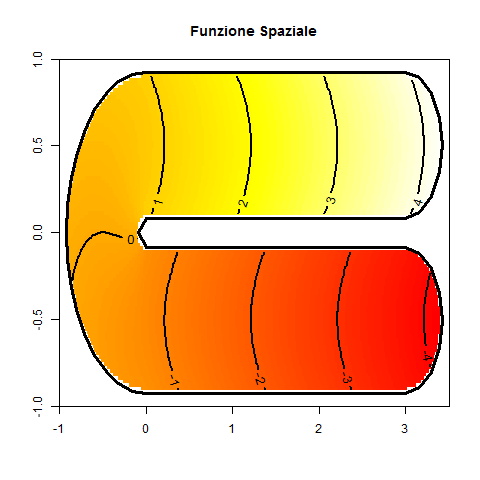
\includegraphics[width=0.44\textwidth]{Immagini/DomCinizio/DomC_fstest.png}   
	\caption{Funzione spaziale $g(\protect\underline{p})$}
	\label{fig:domC_fstest}
\end{figure}


\section{Triangolazione e istanti temporali}
Nel dominio a forma di C non sono presenti punti spaziali definiti dalla natura del problema (come possono essere i comuni per la provincia di Venezia), quindi è stato necessario ricavarli. Sono stati generati casualmente 150 punti all'interno del rettangolo $[-1,+3.5] \times [-1,+1]$ e di questi sono stati considerati validi solo quelli che ricadevano all'interno del dominio. Non è stata usata la descrizione della frontiera presente in \textit{mgcv}, ma una versione diversa che permette di avere punti anche nella parte rettilinea del bordo.
\begin{figure}[t]
	\centering
	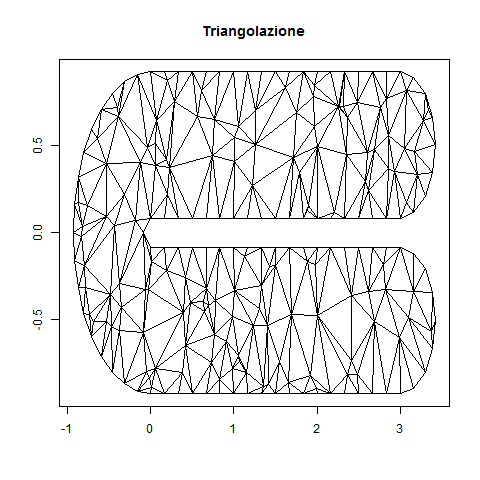
\includegraphics[width=0.44\textwidth]{Immagini/DomCinizio/DomC_Triangolazione.png}
	\caption{Triangolazione del dominio a forma di C}
	\label{fig:domC_triang}
\end{figure}
In fig. \ref{fig:domC_triang} è riportata la triangolazione ottenuta grazie al pacchetto R \textit{RTriangle}. Come basi in spazio sono stati usati gli elementi finiti lineari definiti su questa triangolazione. In tutti gli esempi che seguiranno sarà considerata questa descrizione del dominio, che è formata da 241 punti (pari anche al numero di basi spaziali $N$). Di questi, 108 sono di frontiera e i restanti 133 corrispondono agli $n$ punti sui quali saranno disponibili i dati.

Come intervallo temporale di variazione dei dati è stato scelto $[0,2\pi]$ per sfruttare la periodicità del coseno. All'interno di questo intervallo sono stati ricavati 9 istanti temporali equidistanti tra di loro, quindi uno ogni $\frac{\pi}{4}$. Si è scelto di fissare come basi in tempo le B-splines cubiche. Il numero di basi $M$ è uguale al numero di istanti temporali a disposizione $m$, quindi 9. 
\newpage
\section{Caso senza covariata}

\subsection{Ricerca del miglior $\protect\underline{\lambda}$}
Nei punti e negli istanti temporali disponibili i dati sono stati ricavati dalla funzione esatta con l'aggiunta del rumore:
$$
z_{ij}=g(\underline p_{i})cos(t_j) + \varepsilon_{ij} \qquad \forall i \in 1\ldots n, \forall j \in 1\ldots m
$$
dove
$$
\varepsilon_{ij}\stackrel{\mathrm{iid}}{\sim}N(0,0.5^2) \qquad \forall i \in 1\ldots n, \forall j \in 1\ldots m \ .
$$

Per poter eseguire una analisi ottimale, come primo passo è necessario scegliere i valori per $\lambda$ ottimizzando l'indice $\mathrm{GCV}(\underline \lambda)$ come riportato in eq. \ref{eq:GCV}. In queste analisi $\lambda_S$ e $\lambda_T$ sono sempre espressi in potenze di 10. Per trovare dei buoni valori per i parametri si procede per tentativi, creando due insiemi discreti di variazione per $\log_{10}\lambda_S$ e $\log_{10}\lambda_T$ e minimizzando sui $\underline \lambda$ corrispondenti al prodotto cartesiano tra di essi. Il procedimento viene iterato qualche volta (a causa dell'alto costo computazionale non è opportuno eseguire troppe iterazioni) rendendo la griglia sempre più fitta. In particolare, nel primo caso i valori sono distanziati di 1, poi (una volta che è possibile centrare gli intervalli in base al risultato precedente) di 0.25 e 0.125.
\newline
\begin{table}[h]
\renewcommand{\arraystretch}{1.3}
\setlength{\tabcolsep}{2mm}
\centering
	\begin{tabular}{!{\vrule width 1.2pt}c!{\vrule width 1.2pt}c!{\vrule width 1.2pt}}
	\noalign{\hrule height 1.2pt}
	Intervalli per $\log_{10}\lambda_S$ e $\log_{10}\lambda_T$& Miglior valore											\\
	\noalign{\hrule height 1.2pt}
	$\log_{10}\lambda_S \in \{-5,-4,\ldots,+1\}$ 	& \multirow{2}{*}{$\underline \lambda = (10^{0},10^{-3})$} 			\\
	\cline{1-1}
	$\log_{10}\lambda_T \in \{-5,-4,\ldots,+1\}$		& 															\\	
	\noalign{\hrule height 1.2pt}
	$\log_{10}\lambda_S \in \{-1,-0.75,\ldots,+1\}$ 	& \multirow{2}{*}{$\underline \lambda = (10^{-0.5},10^{-3.25})$} 		\\
	\cline{1-1}
	$\log_{10}\lambda_T \in \{-4,-3.75,\ldots,-2\}$	& 															\\	
	\noalign{\hrule height 1.2pt}
	$\log_{10}\lambda_S \in \{-1,-0.875,\ldots,+0\}$ 	& \multirow{2}{*}{$\underline \lambda = (10^{-0.375}, 10^{-3.25})$}	\\
	\cline{1-1}
	$\log_{10}\lambda_T \in \{-3.75,-3.625,\ldots,-2.75\}$		& 												\\	
	\noalign{\hrule height 1.2pt}
	\end{tabular}
\caption{Analisi di $\mathrm{GCV}(\protect\underline{\lambda})$ per il dominio a forma di C, caso senza covariata}
\label{tab:DomC}
\end{table}

\subsection{Risultati}
L'analisi è stata eseguita con $\underline \lambda = (10^{-0.375}, 10^{-3.25})$ e la stima della funzione si è rivelata molto buona. In fig. \ref{fig:DomC_ris} sono riportati i confronti tra funzione reale e stimata nei primi istanti di tempo (la scala di colori è stata resa uniforme tra tutti i grafici). Si può notare come la funzione stimata sia effettivamente molto simile a quella reale.
\newpage
\begin{figure}[H]
\centering
	\subfigure[Funzione reale a $t=0$]
   {
	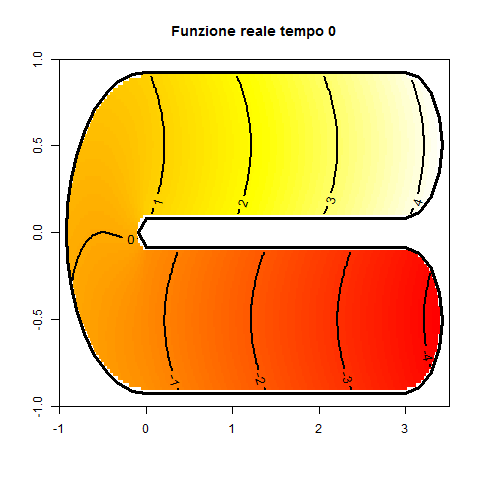
\includegraphics[width=0.40\textwidth]{Immagini/DomC/DomC_0reale.png}   
   }
	\subfigure[Funzione stimata a $t=0$]
   {
	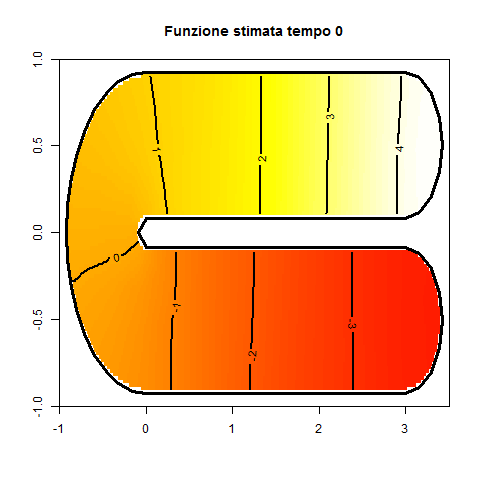
\includegraphics[width=0.40\textwidth]{Immagini/DomC/DomC_0stimata.png}
   }
   \subfigure[Funzione reale a $t=\frac{\pi}{4}$]
   {
	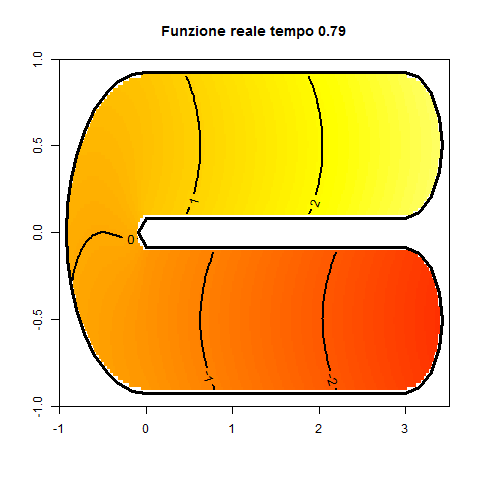
\includegraphics[width=0.40\textwidth]{Immagini/DomC/DomC_1reale.png}   
   }
	\subfigure[Funzione stimata a $t=\frac{\pi}{4}$]
   {
	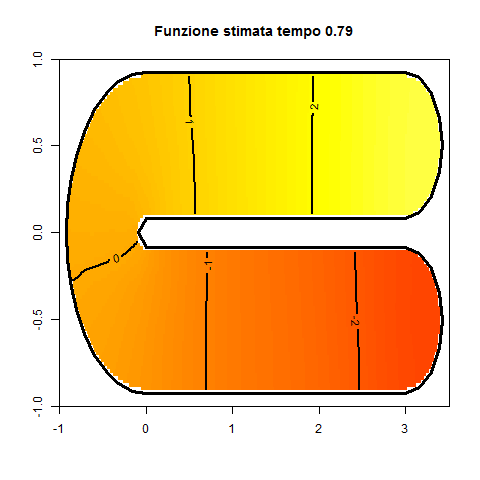
\includegraphics[width=0.40\textwidth]{Immagini/DomC/DomC_1stimata.png}
   }
   \subfigure[Funzione reale a $t=\frac{\pi}{2}$]
   {
	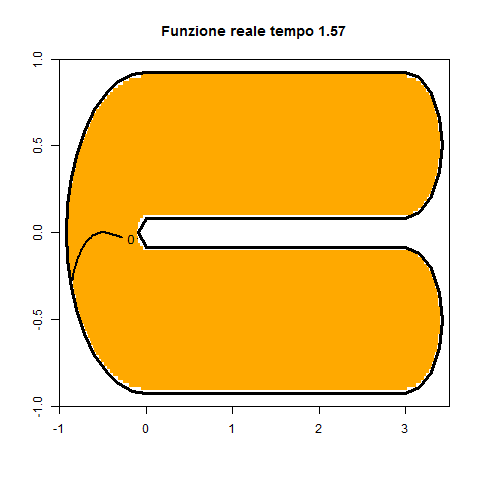
\includegraphics[width=0.40\textwidth]{Immagini/DomC/DomC_2reale.png}   
   }
	\subfigure[Funzione stimata a $t=\frac{\pi}{2}$]
   {
	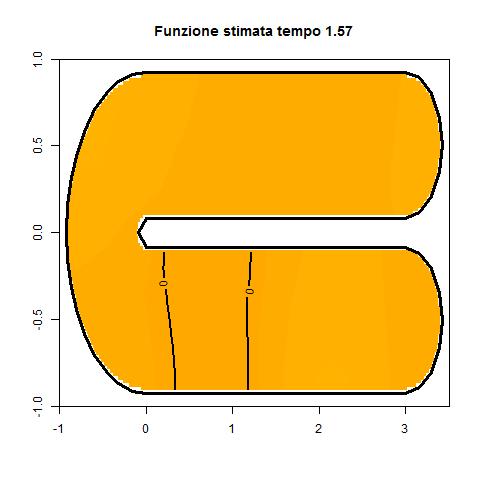
\includegraphics[width=0.40\textwidth]{Immagini/DomC/DomC_2stimata.png}
   }
	\caption{Stime della funzione $f(\protect\underline{p},t)$ ad alcuni istanti di tempo, caso senza covariata}
	\label{fig:DomC_ris}
\end{figure}

In fig. \ref{fig:DomC_ris2} si ha il confronto dell'evoluzione temporale in alcuni nodi della triangolazione. Oltre alla curva stimata è tracciata la reale, che è una cosinusoide di ampiezza nota (grazie alla perfetta conoscenza di $g(\underline p)$) riportata con i grafici. I punti rossi corrispondono al dato sporcato dal rumore. Tanto più è vicina a zero l'ampiezza della curva, tanto più il rumore influenza la stima poiché più rilevante (infatti, in fig. \ref{fig:DomC_ris}, le curve di livello dove la funzione reale è vicina a zero sono le più diverse da quelle corrette). Tuttavia, anche nel caso con ampiezza vicina al valore massimo di $g(\underline p)$ in fig. \ref{fig:DomC_ris2C}, la curva stimata non è una perfetta interpolazione dei dati e coglie il vero andamento temporale della funzione. Si può concludere quindi che la stima è molto buona, sebbene più confusa nella parte centrale del dominio a forma di C.

\begin{figure}[t]
	\centering
	\subfigure[Ampiezza $0.3486$]
	{
	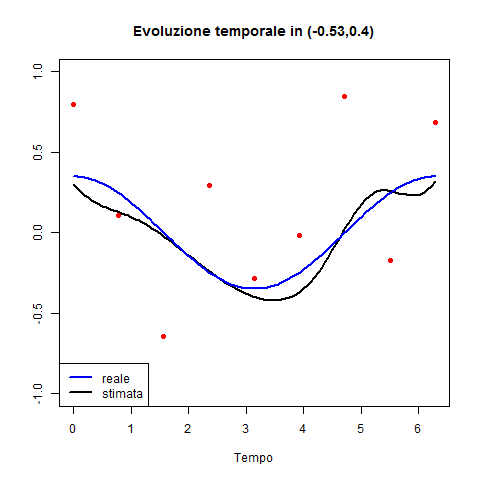
\includegraphics[width=0.31\textwidth]{Immagini/DomC/tfissato1.png}   
   }
	\subfigure[Ampiezza $1.3819$]
   {
	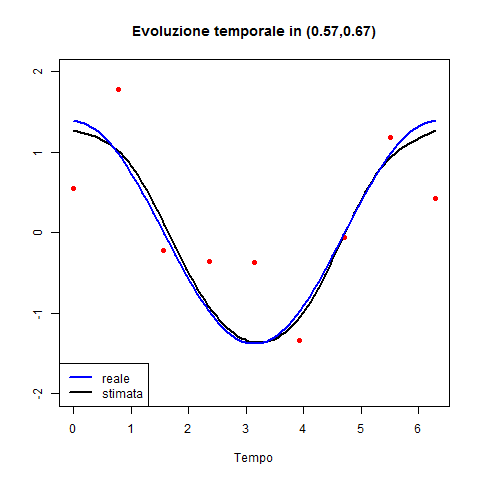
\includegraphics[width=0.31\textwidth]{Immagini/DomC/tfissato2.png}
   }
   \subfigure[Ampiezza $4.1648$]
   {
	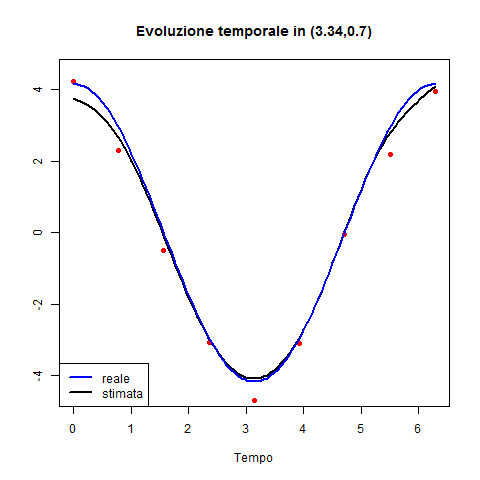
\includegraphics[width=0.31\textwidth]{Immagini/DomC/tfissato3.png}  
	\label{fig:DomC_ris2C} 
   } 
	\caption{Evoluzione temporale in alcuni nodi della triangolazione, caso senza covariata}
	\label{fig:DomC_ris2}
\end{figure}

\subsection{Analisi dei residui}
Nella costruzione del modello spiegata nel dettaglio nel capitolo \ref{cap:modello} si ipotizza che il rumore aggiunto al dato funzionale sia generato da una variabile aleatoria di media nulla e varianza $\sigma^2$. Quindi si ha l'ipotesi di omoschedasticità che deve essere verificata per validare i risultati ottenuti, analogamente a quanto si fa per i modelli di regressione lineare. In questo caso il processo di generazione dei dati è perfettamente noto e il rumore rispetta questa ipotesi poiché generato da una normale con parametri fissi. Tuttavia, per introdurre una prassi che deve essere rispettata quando si controllano i risultati di questo algoritmo, anche in questo caso in cui già a priori si ha la certezza della validità dell'ipotesi di omoschedasticità è opportuno eseguire l'analisi dei residui.

Ad ogni dato è possibile associare il residuo
$$
e_{ij}=z_{ij}-\hat{z}_{ij}
$$
che, tramite opportuni scatterplot, è impiegato nella verifica dell'ipotesi di omogeneità della varianza.
\newpage
\begin{figure}[t]
	\centering
	\subfigure[$z_{ij}$ vs $e_{ij}$]
	{
	\includegraphics[width=0.46\textwidth]{Immagini/DomC/Scatterplot4.png}  
	\label{fig:DomC_residuiA} 
   }
	\subfigure[$\hat{z}_{ij}$ vs $e_{ij}$]
   {
	\includegraphics[width=0.46\textwidth]{Immagini/DomC/Scatterplot5.png}
   }
	\caption{Scatterplot dei residui, caso senza covariata}
	\label{fig:DomC_residui}
\end{figure}
Dall'analisi dei grafici in fig. \ref{fig:DomC_residui} si può facilmente capire che non si ha una cattiva dispersione dei residui attorno allo zero. Quindi, come ci si aspettava, l'ipotesi di omoschedasticità può essere considerata valida.

Inoltre, il grafico in fig. \ref{fig:DomC_residuiA} permette di evidenziare una delle particolarità dello smoothing associato all'algoritmo. I residui negativi più bassi sono in corrispondenza dei dati minori e, analogamente, i residui positivi più alti sono in corrispondenza dei dati maggiori. Questo è dovuto allo smoothing imposto dal modello, che tende a smussare la funzione $f(\underline{p},t)$ nei suoi massimi e minimi: come si può notare in fig. \ref{fig:DomC_ris2C} in questi punti si ha la maggior distanza tra la curva reale e quella stimata.

\section{Caso con covariata}

\subsection{Generazione della covariata e ricerca del miglior $\protect\underline{\lambda}$}
Nel problema della stima della funzione $f(\underline p,t)=g(\underline p)cos(t)$ non sono presenti covariate. Quindi per poter provare il modello in questo caso, è stato necessario generare valori da assumere come covariata in ogni punto spaziale ed istante temporale in cui si hanno le misurazioni della risposta.
\newpage
In definitiva i dati sono così formati:
$$
z_{ij}=g(\underline p_{i})cos(t_j) + \beta w_{ij} + \varepsilon_{ij} \qquad \forall i \in 1\ldots n, \forall j \in 1\ldots m
$$
dove covariata e rumore sono generate da due normali tra loro indipendenti:
$$
w_{ij}\stackrel{\mathrm{iid}}{\sim}N(0,1) \qquad \forall i \in 1\ldots n, \forall j \in 1\ldots m
$$
$$
\varepsilon_{ij}\stackrel{\mathrm{iid}}{\sim}N(0,0.5^2) \qquad \forall i \in 1\ldots n, \forall j \in 1\ldots m
$$
e $\beta$ è fissato a 1. Se il modello è buono, c'è da aspettarsi che la parte di funzione stimata senza covariata sia vicina a $f(\underline p,t)$ e che $\hat{\beta}$ si avvicini a 1.
 
Anche in questo caso è necessaria una analisi preliminare per fissare i valori per $\lambda$ ottimizzando l'indice $\mathrm{GCV}(\underline \lambda)$, che nel caso con covariata si differenzia dal precedente solo per la forma della \textit{smoothing matrix}. In tab. \ref{tab:DomC_covar} sono riportati i risultati ricavati adattando lo stesso approccio del caso senza covariata.
\newline
\newline
\begin{table}[htbp]
\renewcommand{\arraystretch}{1.3}
\setlength{\tabcolsep}{2mm}
\centering
	\begin{tabular}{!{\vrule width 1.2pt}c!{\vrule width 1.2pt}c!{\vrule width 1.2pt}}
	\noalign{\hrule height 1.2pt}
	Intervalli per $\log_{10}\lambda_S$ e $\log_{10}\lambda_T$& Miglior valore											\\
	\noalign{\hrule height 1.2pt}
	$\log_{10}\lambda_S \in \{-5,-4,\ldots,+1\}$ 	& \multirow{2}{*}{$\underline \lambda = (10^{0},10^{-4})$} 			\\
	\cline{1-1}
	$\log_{10}\lambda_T \in \{-5,-4,\ldots,+1\}$		& 															\\	
	\noalign{\hrule height 1.2pt}
	$\log_{10}\lambda_S \in \{-1,-0.75,\ldots,+1\}$ 	& \multirow{2}{*}{$\underline \lambda = (10^{0.25},10^{-3.75})$} 		\\
	\cline{1-1}
	$\log_{10}\lambda_T \in \{-5,-4.75,\ldots,-3\}$	& 															\\	
	\noalign{\hrule height 1.2pt}
	$\log_{10}\lambda_S \in \{-0.25,-0.125,\ldots,+0.75\}$ 	& \multirow{2}{*}{$\underline \lambda = (10^{-0.125}, 10^{-3.25})$}	\\
	\cline{1-1}
	$\log_{10}\lambda_T \in \{-4.25,-4.125,\ldots,-3.25\}$		& 												\\	
	\noalign{\hrule height 1.2pt}
	\end{tabular}
\caption{Analisi di $\mathrm{GCV}(\protect\underline{\lambda})$ per il dominio a forma di C, caso con covariata}
\label{tab:DomC_covar}
\end{table}
\newline
\newline
Procedendo per tentativi, si può notare come i valori si sono rivelati molto simili al caso senza covariata riportato in \ref{tab:DomC}, facendo pensare che la stima della funzione $f(\underline p,t)$, cioè della parte non spiegata dalla covariata, possa essere molto vicina a quella stimata nel caso senza covariata e, quindi, a quella reale.

\subsection{Risultati}
Eseguendo l'analisi con $\underline \lambda = (10^{-0.125}, 10^{-3.25})$ questa ipotesi è confermata e si trova una buona stima della funzione. In fig. \ref{fig:DomCcovar_ris} si hanno i grafici dei primi istanti di tempo (si ricorda che la funzione tracciata non contiene la parte spiegata dalla covariata, ma solo la stima di $f(\underline p,t)$). 
\newpage
\begin{figure}[H]
\centering
\subfigure[Funzione reale a $t=0$]
   {
	\includegraphics[width=0.40\textwidth]{Immagini/DomCCovar/DomCcovar_0reale.png}   
   }
\subfigure[Funzione stimata a $t=0$]
   {
	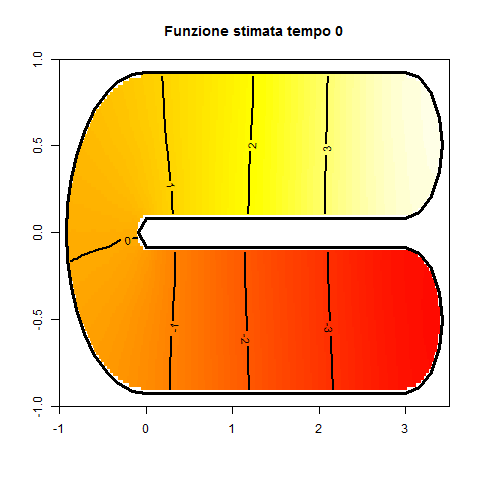
\includegraphics[width=0.40\textwidth]{Immagini/DomCCovar/DomCcovar_0stimata.png}
   }
\subfigure[Funzione reale a $t=\frac{\pi}{4}$]
   {
	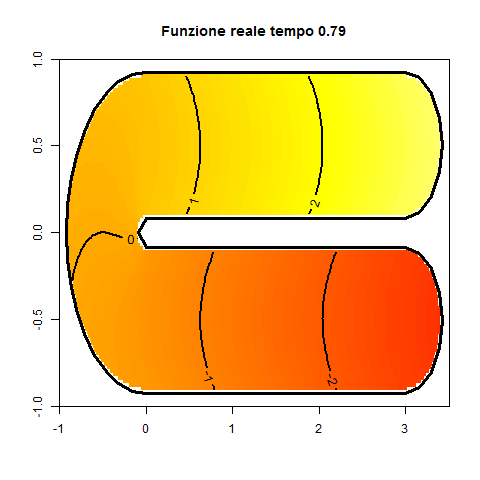
\includegraphics[width=0.40\textwidth]{Immagini/DomCCovar/DomCcovar_1reale.png}   
   }
\subfigure[Funzione stimata a $t=\frac{\pi}{4}$]
   {
	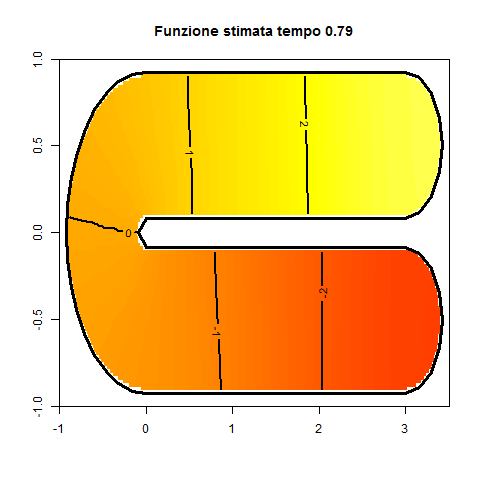
\includegraphics[width=0.40\textwidth]{Immagini/DomCCovar/DomCcovar_1stimata.png}
   }
\subfigure[Funzione reale a $t=\frac{\pi}{2}$]
   {
	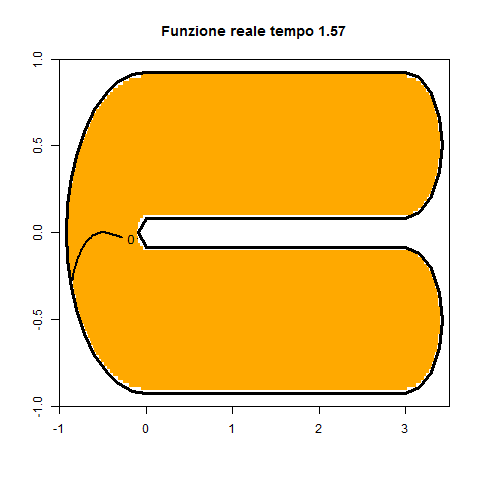
\includegraphics[width=0.40\textwidth]{Immagini/DomCCovar/DomCcovar_2reale.png}   
   }
\subfigure[Funzione stimata a $t=\frac{\pi}{2}$]
   {
	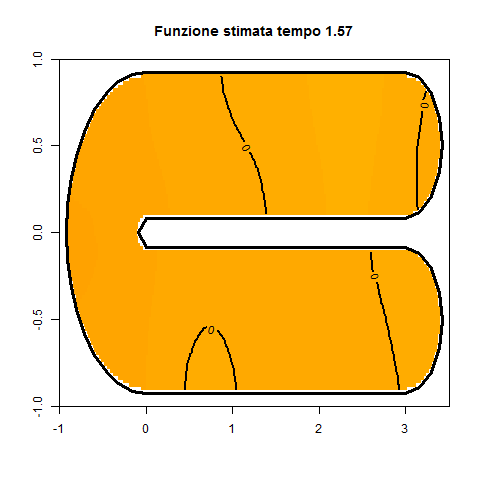
\includegraphics[width=0.40\textwidth]{Immagini/DomCCovar/DomCcovar_2stimata.png}
   }
\caption{Stime della funzione $f(\protect\underline{p},t)$ ad alcuni istanti di tempo, caso con covariata}
\label{fig:DomCcovar_ris}
\end{figure}

In fig. \ref{fig:DomCcovar_ris2}, analogamente a quanto fatto nel caso senza covariata, si hanno i grafici dell'evoluzione temporale della funzione in alcuni punti spaziali. I punti rossi tracciati corrispondono alla parte di dato senza il termine dovuto alla covariata. Le conclusioni sono le stesse del caso senza covariata: la stima è ben riuscita e la vera variazione temporale è stata colta dal modello. Tuttavia, avvicinandosi alla parte centrale del dominio, si ha una maggiore influenza del rumore.

\begin{figure}[t]
	\centering
	\subfigure[Ampiezza $0.2810$]
	{
	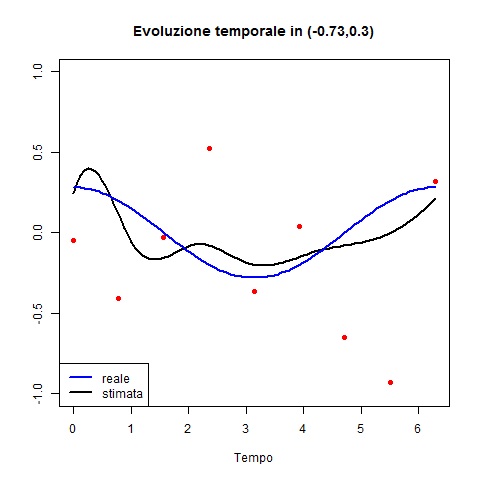
\includegraphics[width=0.31\textwidth]{Immagini/DomCCovar/tfissato1.png}   
   }
	\subfigure[Ampiezza $1.2761$]
   {
	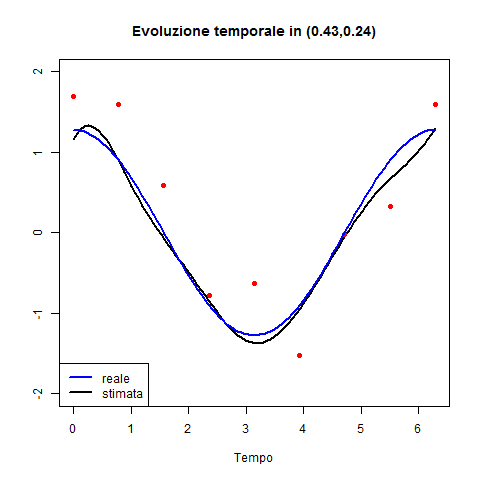
\includegraphics[width=0.31\textwidth]{Immagini/DomCCovar/tfissato2.png}
   }
   \subfigure[Ampiezza $3.8577$]
   {
	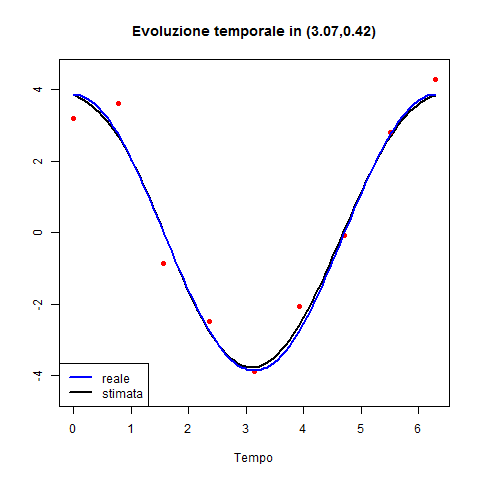
\includegraphics[width=0.31\textwidth]{Immagini/DomCCovar/tfissato3.png}   
   } 
	\caption{Evoluzione temporale in alcuni nodi della triangolazione, caso con covariata}
	\label{fig:DomCcovar_ris2}
\end{figure}

Dai grafici precedenti si può concludere che la stima della parte funzionale della risposta sia effettivamente una buona approssimazione della reale. Tuttavia occorre verificare anche che il contributo delle covariata sia ben riconosciuto dal modello, e per questo basta controllare il valore stimato di $\beta$. Si ha:
$$
\hat{\beta} \approx 1.005 \ ,
$$
valore vicinissimo al reale.

\subsection{Analisi dei residui e test d'ipotesi per $\beta$}
Sarebbe interessante eseguire un test del tipo
$$
\begin{cases}
H_0: & \beta=1 \\
H_1: & \beta \not = 1
\end{cases}
$$
per poter controllare con una data significatività se il valore stimato corrisponde a quello reale. Tuttavia è necessario controllare prima le ipotesi del modello e verificare se è possibile attribuire la normalità ai residui. Analogamente a quanto fatto nel caso senza covariata, siamo già certi che tutte queste ipotesi siano valide per come sono stati costruiti i dati. Tuttavia, per completezza, è necessario eseguire l'analisi dei residui anche in questo caso.

\begin{figure}[t]
	\centering
	\subfigure[$z_{ij}$ vs $e_{ij}$]
	{
	\includegraphics[width=0.45\textwidth]{Immagini/DomCCovar/Scatterplot4.png}   
   }
	\subfigure[$\hat{z}_{ij}$ vs $e_{ij}$]
   {
	\includegraphics[width=0.45\textwidth]{Immagini/DomCCovar/Scatterplot5.png}
   }
	\caption{Scatterplot dei residui, caso con covariata}
	\label{fig:DomCcovar_residui}
\end{figure}

Per quanto riguarda l'omoschedasticità, in fig. \ref{fig:DomCcovar_residui} si hanno gli scatterplot dei residui. Non si hanno problemi riguardo all'ipotesi di varianza uniforme e valgono le stesse considerazioni riportate nel caso senza covariata.

\begin{figure}[h]
	\centering
	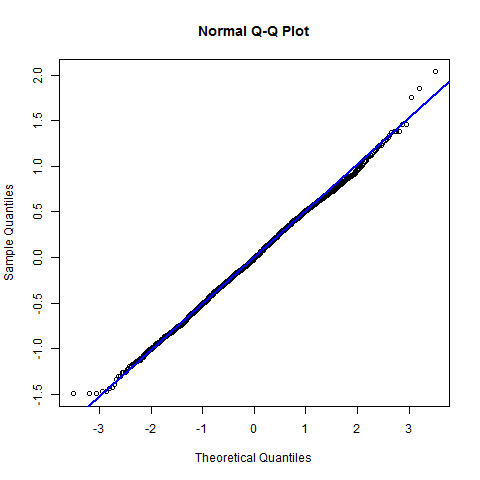
\includegraphics[width=0.45\textwidth]{Immagini/DomCCovar/QQplot.png}   
   \caption{QQplot dei residui, caso con covariata}
	\label{fig:DomCcovar_qqplot}
\end{figure}
Riguardo alla normalità, sia in base al QQplot dei residui riportato in fig. \ref{fig:DomCcovar_qqplot} (che si adatta alla retta eccetto per qualche punto nelle code) sia in base al p-value del Shapiro-Wilk test (0.1259) si può concludere che i residui possono essere considerati gaussiani. Quindi è possibile costruire un intervallo di confidenza approssimato al $95\%$ per $\beta$ (eliminando il termine di distorsione) con quanto ricavato in sez. \ref{sec:IC}. Ne risulta:
$$
\beta \in [0.9843;1.0259]
$$
che contiene 1. L'ipotesi $H_0$ è accettata.



\chapter{Confronto con altri metodi}
\label{cap:confronto}

Il modello STR-PDE rappresenta una generalizzazione del caso puramente spaziale proposto in \cite{art:sangalli} e, come è già stato evidenziato nel capitolo \ref{cap:panoramica}, non è l'unico modello disponibile per l'analisi di dati distribuiti sia in spazio che in tempo. Pertanto è necessario che sia confrontato con le altre principali metodologie presenti in letteratura, al fine di poter dire se e quanto il modello proposto possa rappresentare un miglioramento in questo campo.

Come già riportato nel cap. \ref{cap:panoramica}, l'articolo \cite{art:augustin} propone l'analisi di dati di questo tipo attraverso modelli misti additivi generalizzati (GAMM) di interazione spazio-tempo. Questo metodo è generalizzato, quindi può essere usato per spiegare anche funzioni del valore atteso della risposta. Nel nostro caso, per avvicinarci al caso STR-PDE, si ipotizza che la risposta sia pari alla somma di una funzione e di un eventuale termine con covariata. Alla funzione è associato lo smoothing secondo il prodotto tensoriale dei termini marginali in spazio e tempo con le loro penalizzazioni. Quindi la costruzione dei GAMM è molto simile a quella analizzata in STR-PDE e, mediante il codice implementato nel pacchetto R \textit{mgcv}, è possibile scegliere tra più tipi di modelli. In particolare ne saranno studiati due, i più simili al modello STR-PDE:
\begin{itemize}
\item TPS, in cui sono poste marginalmente \textit{cubic regression splines} in tempo e \textit{thin plate splines} in spazio;
\item SOAP, che considera \textit{cubic regression splines} in tempo e \textit{soap film smoothing} in spazio.
\end{itemize}

Un altro metodo da confrontare è sicuramente il kriging (KRIG) spazio-temporale. Le stime sono ottenute fissando un variogramma separabile e marginalmente esponenziale in spazio e tempo. I parametri del variogramma sono stimati dall'empirico e, successivamente, è possibile calcolare la stima grazie alle funzioni del pacchetto R \textit{gstat}. 

I quattro modelli sono confrontati sull'esempio del dominio a forma di C proposto precedentemente, poiché garantisce di poter conoscere in ogni punto spaziale e ad ogni istante temporale il valore esatto della funzione. La triangolazione e i dati sono gli stessi che sono stati usati nel capitolo \ref{cap:domC}. In aggiunta è stata costruita una griglia spazio-temporale di punti per la validazione: sono stati presi 80 punti equispaziati in $[-1,+3.5]$ per l'ascissa, 40 punti in equispaziati $[-1,+1]$ per l'ordinata e 20 istanti in $[0,2\pi]$ per il tempo. Ovviamente la validazione è stata studiata soltanto sui punti che ricadevano all'interno del dominio a forma di C.

I modelli sono stati confrontati attraverso il Root Mean Square Error ($\mathrm{RMSE}$) prodotto sui punti di validazione. Quindi se se $V$ è l'insieme dei punti della griglia interni al dominio, e $\mathrm{Mod}$ rappresenta la stima ottenuta dal modello, si avrà:
$$
\mathrm{RMSE}_V(\mathrm{Mod})=\sqrt{\frac{\sum_{(\underline p_i,t_i)\in V} (\mathrm{Mod}(\underline p_i,t_i)-g(\underline p_i)cos(t_i))^2}{\mathrm{card}(V)}}
$$ 

Il procedimento è stato iterato 50 volte, per poter escludere possibili effetti particolari dovuti alla generazione del rumore.

\newpage
\section{Caso senza covariata}
Nel caso senza covariata si hanno i risultati riportati in fig. \ref{fig:cfr}, in cui sono stati tracciati i boxplot dei valori di $\mathrm{RMSE}$ raccolti nelle 50 iterazioni per ogni metodo. Subito si nota che l'errore commesso è minore nel caso di STR-PDE, e quindi la stima ottenuta con il modello proposto è la migliore.

Tutto ciò è confermato dai grafici presenti in fig. \ref{fig:confronto_altri_metodi_nocov}. Dai boxplot si nota che l'errore commesso è più alto nei casi di KRIG e TPS, e infatti le stime sono molto distanti dalla funzione reale. Invece SOAP e STR-PDE commettono errori minori, ma tra i due il migliore è STR-PDE, che ha linee di livello più ordinate rispetto a SOAP. 

\begin{figure}[t]
	\centering
	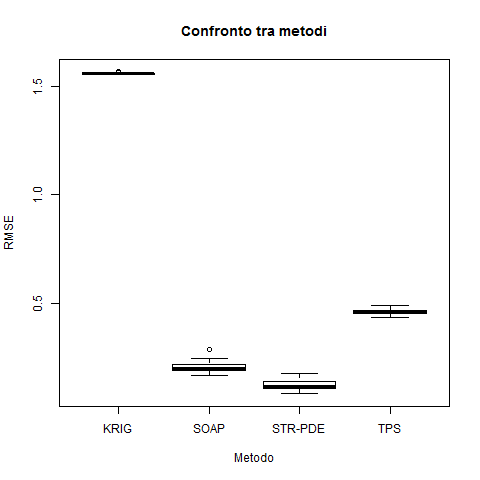
\includegraphics[width=0.60\textwidth]{Immagini/Confronto_metodi.png}   
	\caption{Confronto tra i metodi, caso senza covariata}
	\label{fig:cfr}
\end{figure}

\begin{landscape}
\begin{figure}
\centering
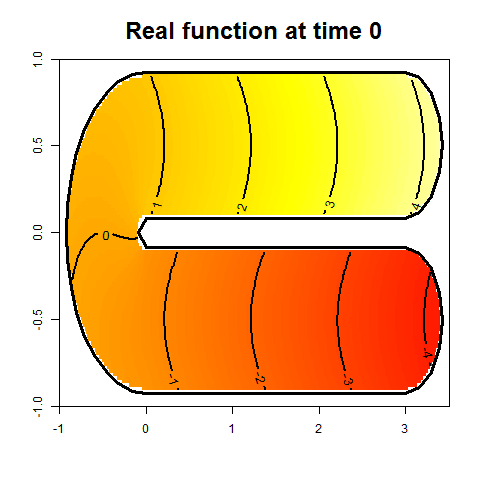
\includegraphics[width=0.25\textwidth]{immagini/simulazioni/REALEtempo1.png}
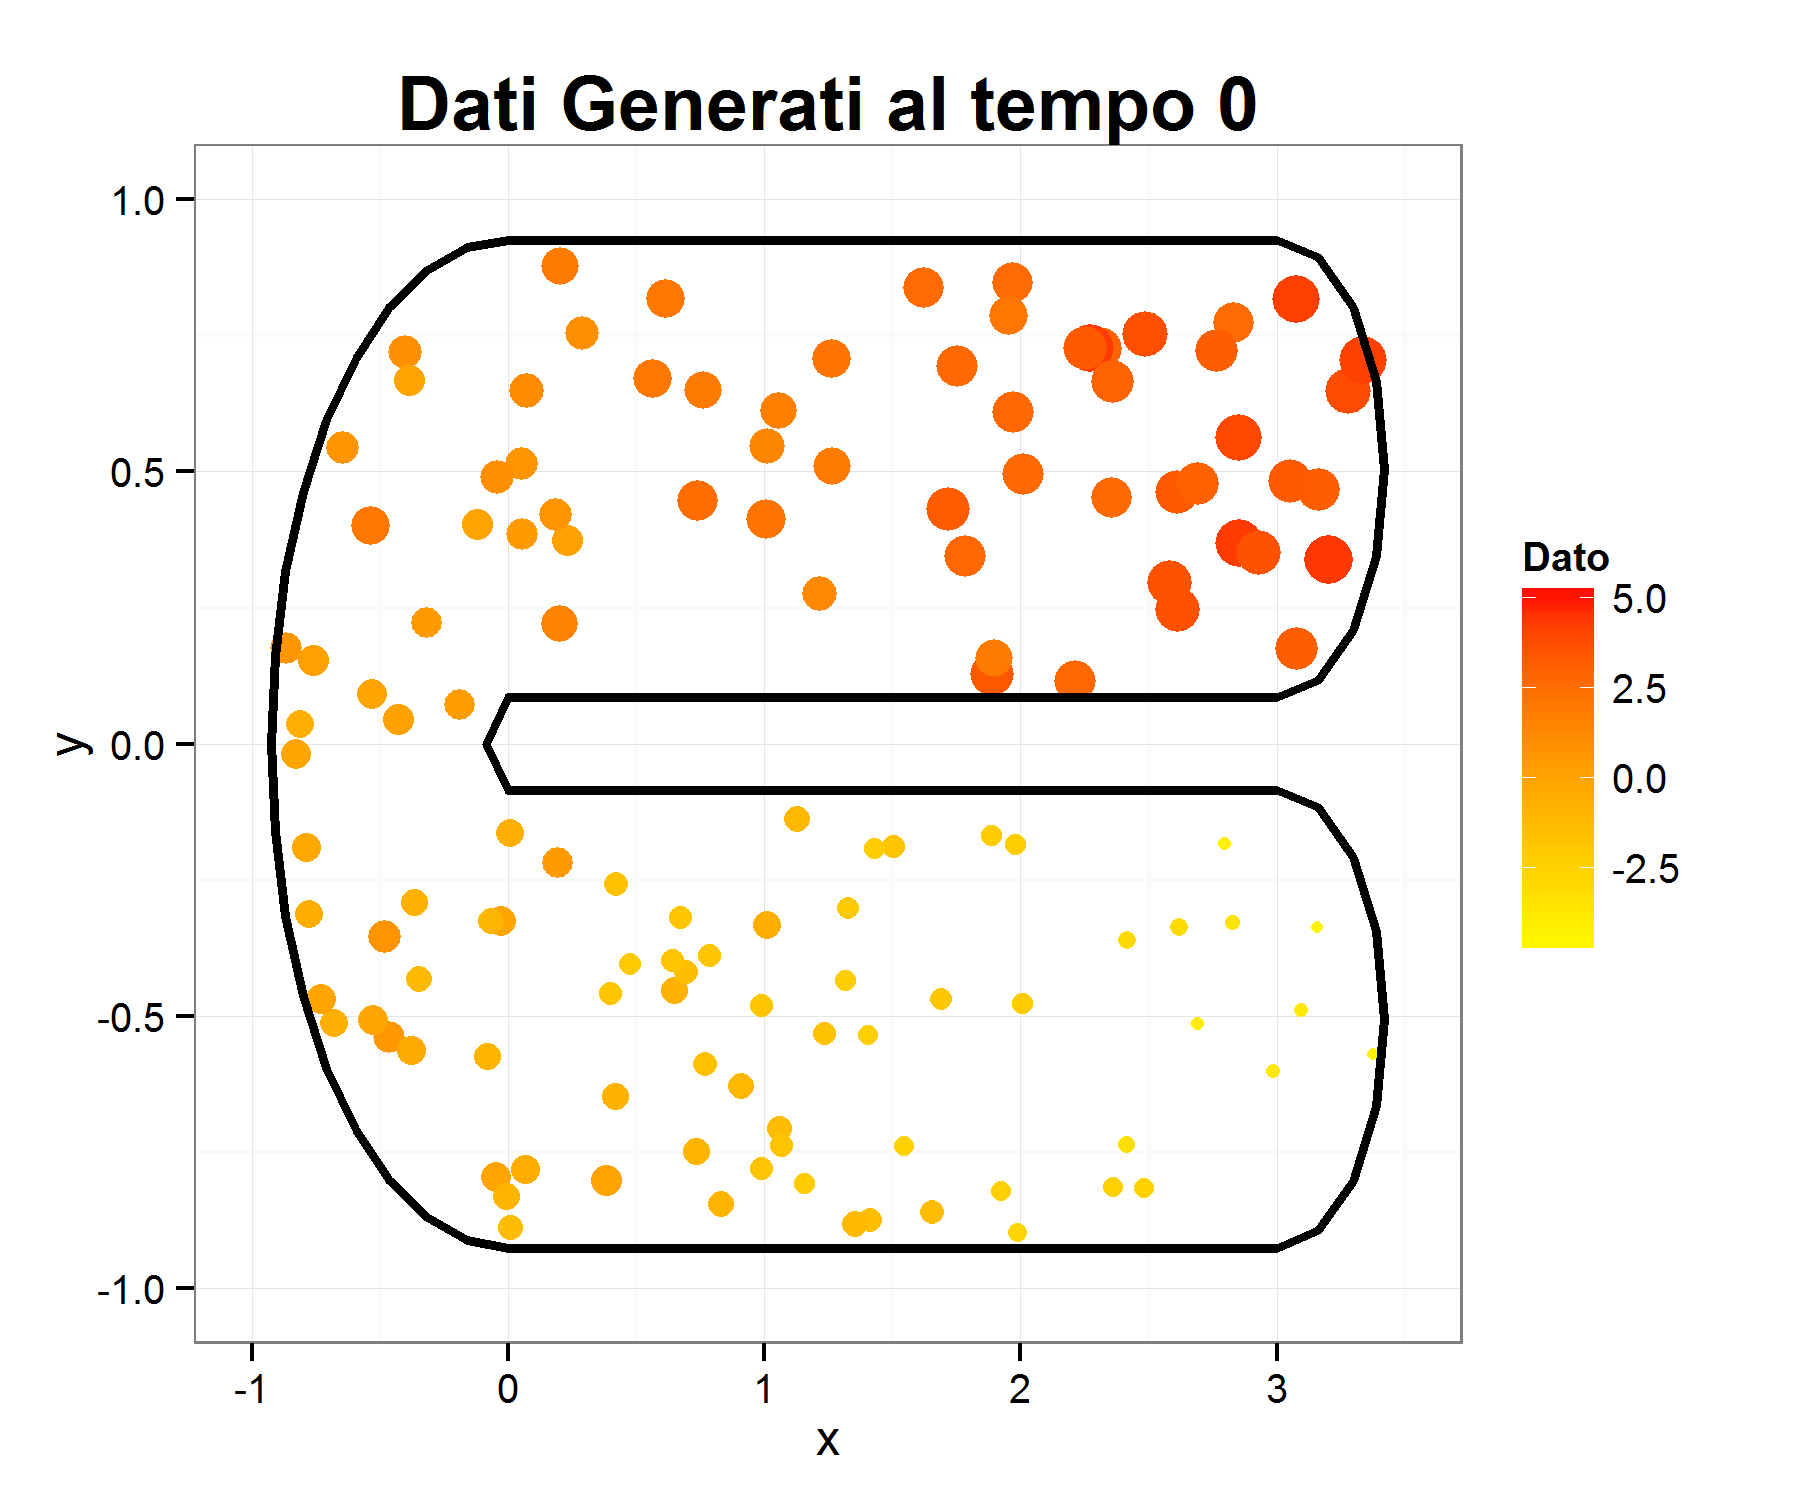
\includegraphics[height=0.25\textwidth]{immagini/simulazioni/Dati_tempo1.png}
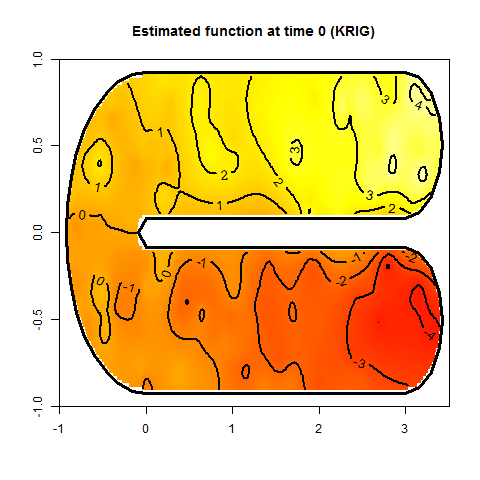
\includegraphics[width=0.25\textwidth]{immagini/simulazioni/KRIGtempo1.png}
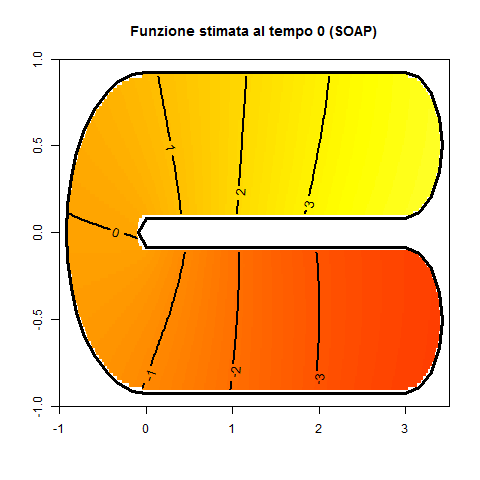
\includegraphics[width=0.25\textwidth]{immagini/simulazioni/SOAPtempo1.png}
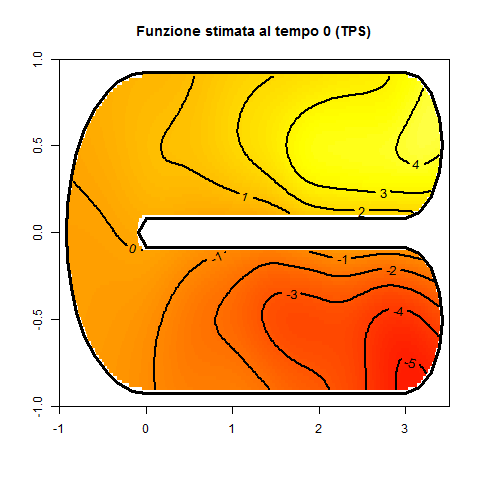
\includegraphics[width=0.25\textwidth]{immagini/simulazioni/TPStempo1.png}
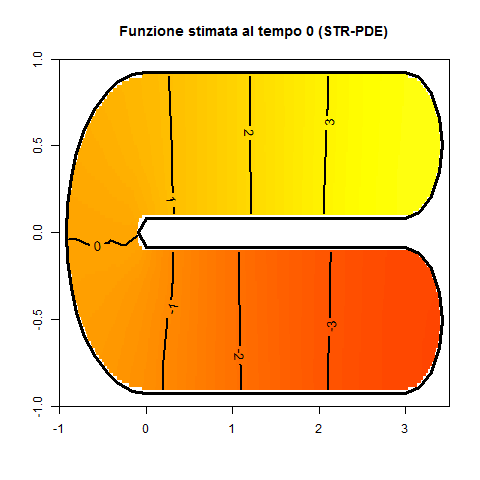
\includegraphics[width=0.25\textwidth]{immagini/simulazioni/STSRtempo1.png}

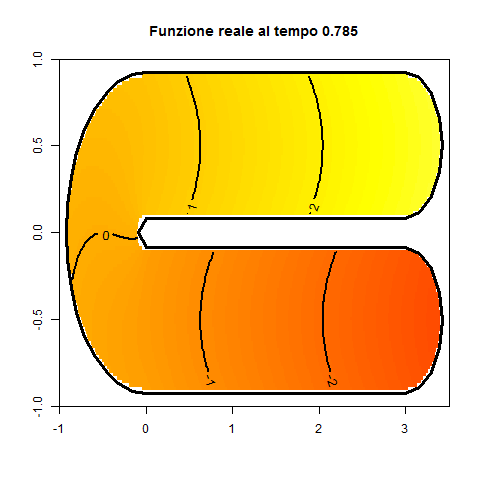
\includegraphics[width=0.25\textwidth]{immagini/simulazioni/REALEtempo2.png}
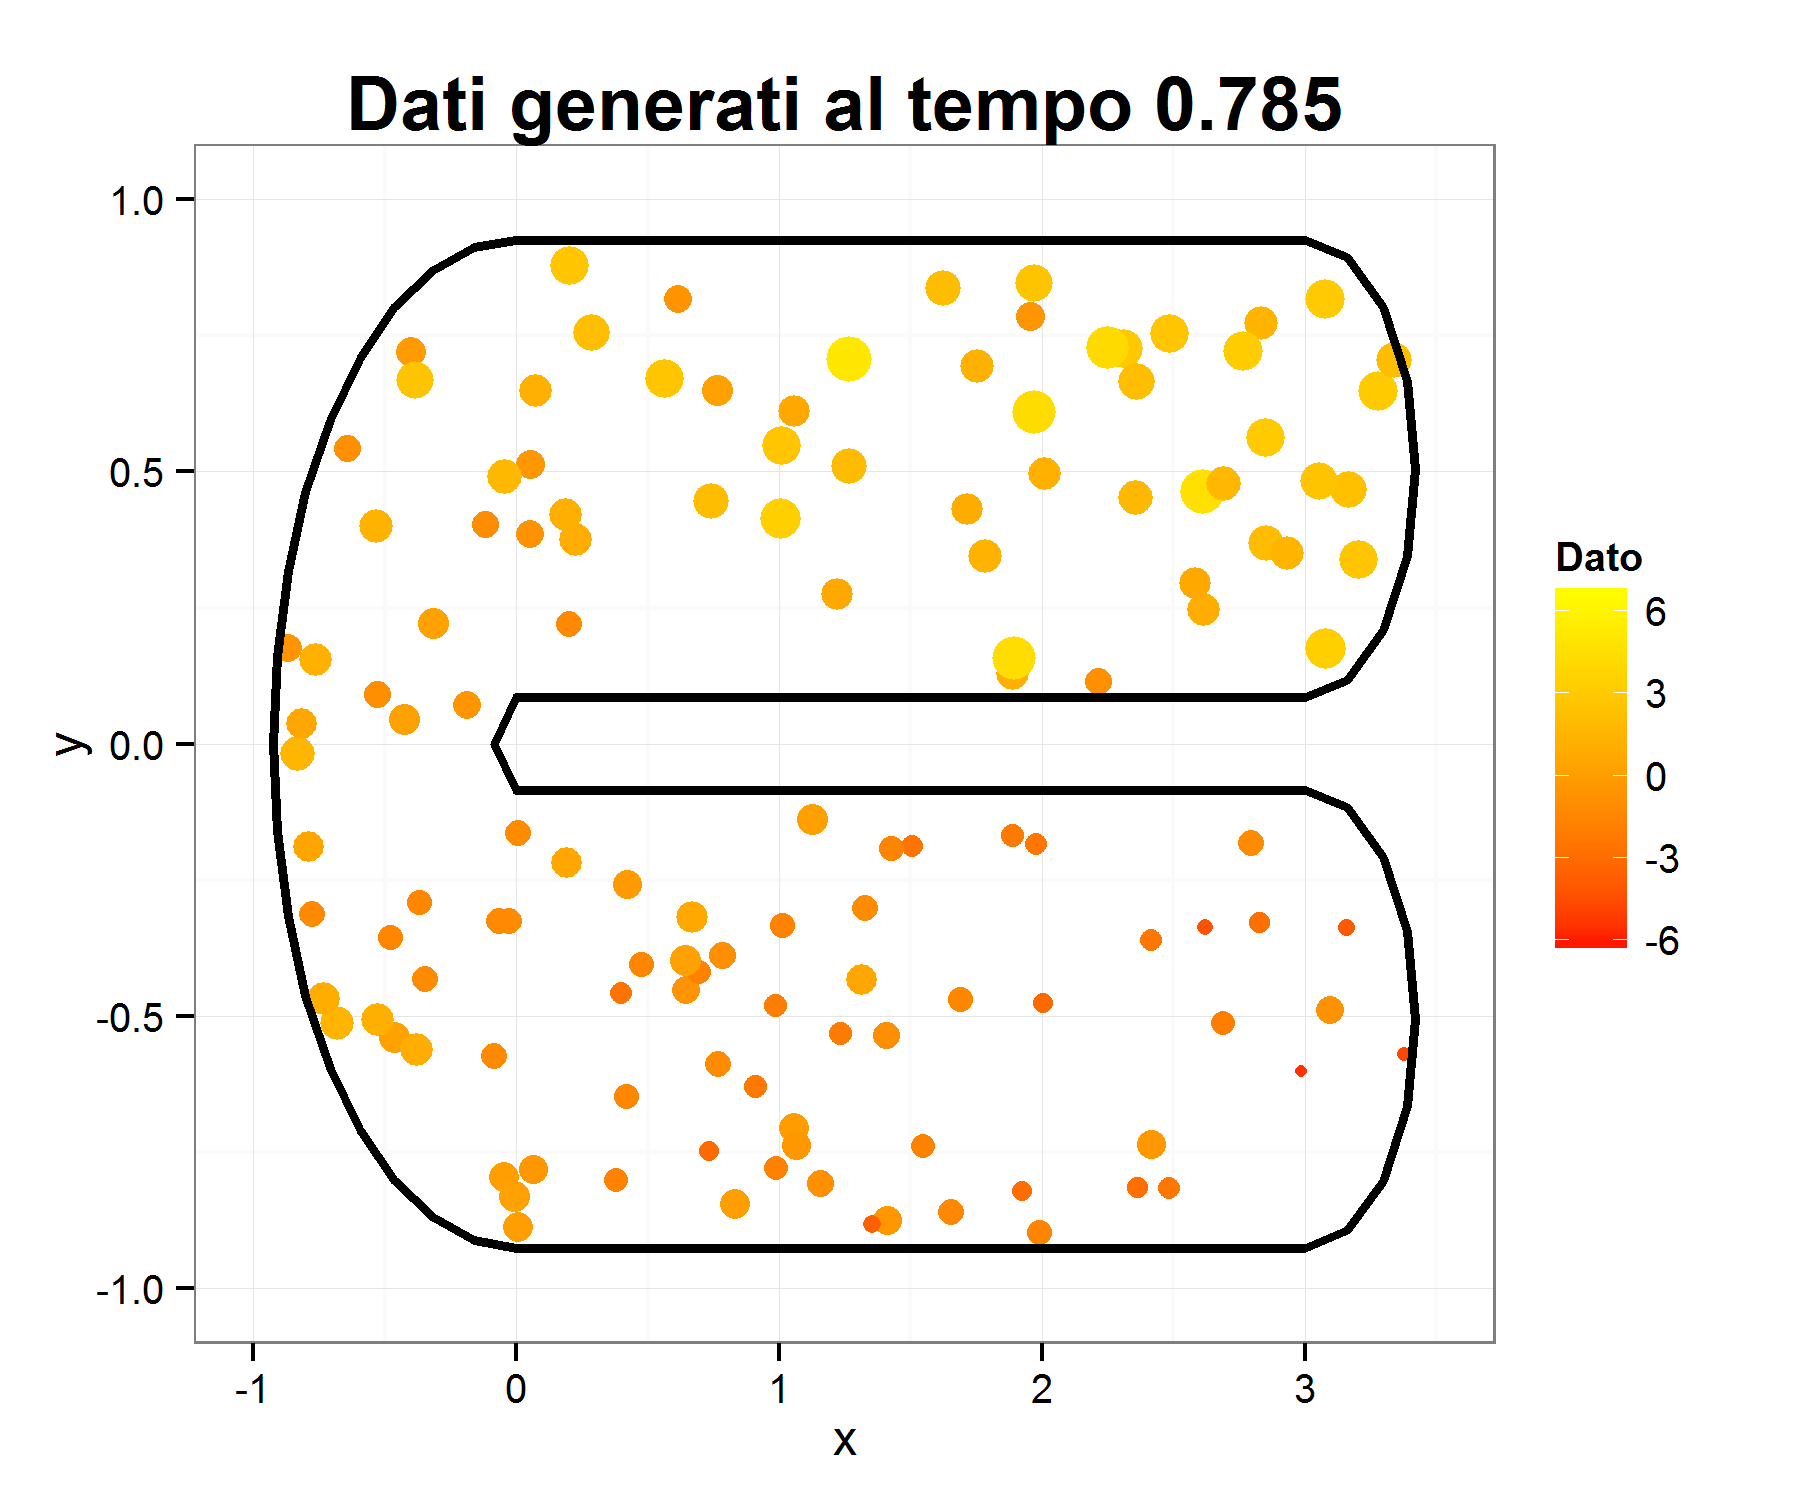
\includegraphics[height=0.25\textwidth]{immagini/simulazioni/Dati_tempo2.png}
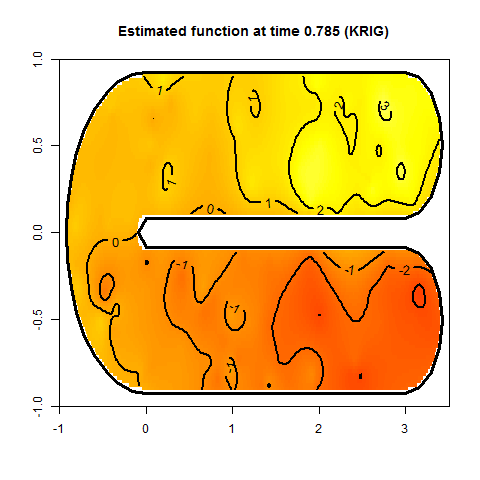
\includegraphics[width=0.25\textwidth]{immagini/simulazioni/KRIGtempo2.png}
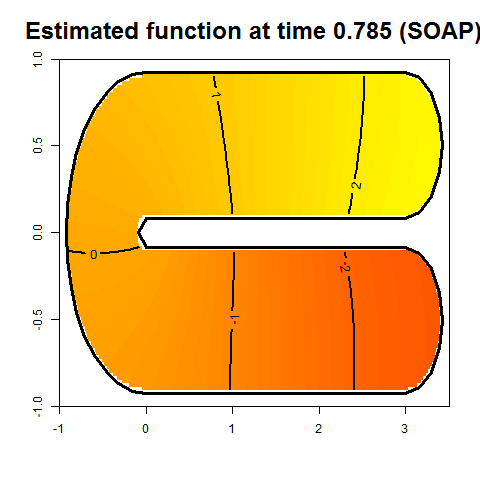
\includegraphics[width=0.25\textwidth]{immagini/simulazioni/SOAPtempo2.png}
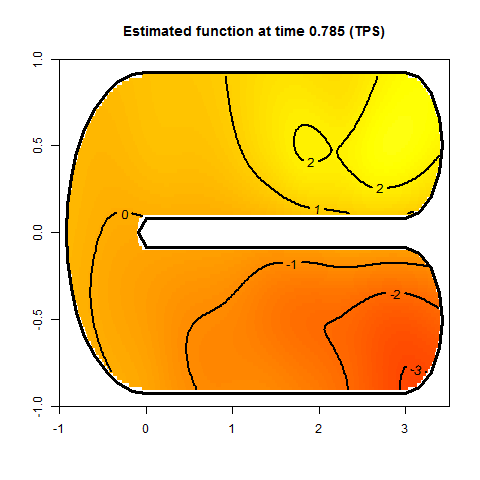
\includegraphics[width=0.25\textwidth]{immagini/simulazioni/TPStempo2.png}
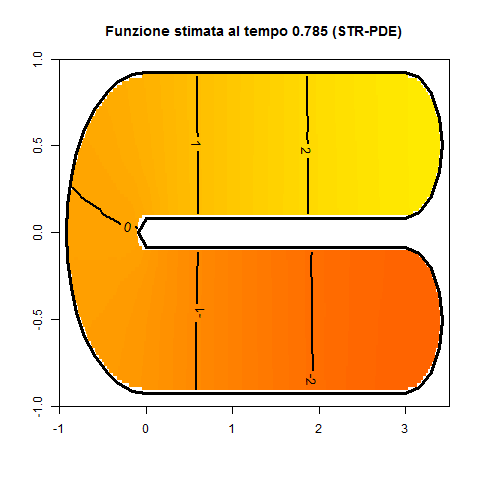
\includegraphics[width=0.25\textwidth]{immagini/simulazioni/STSRtempo2.png}

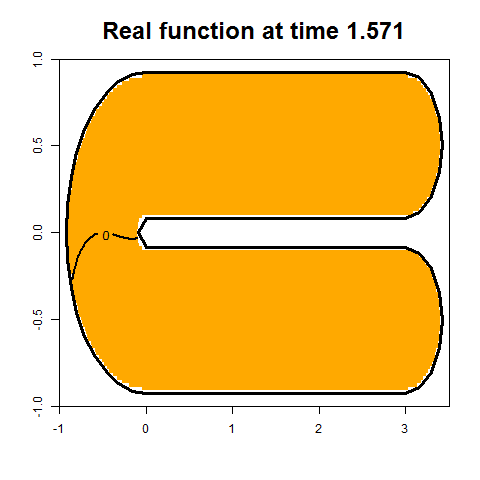
\includegraphics[width=0.25\textwidth]{immagini/simulazioni/REALEtempo3.png}
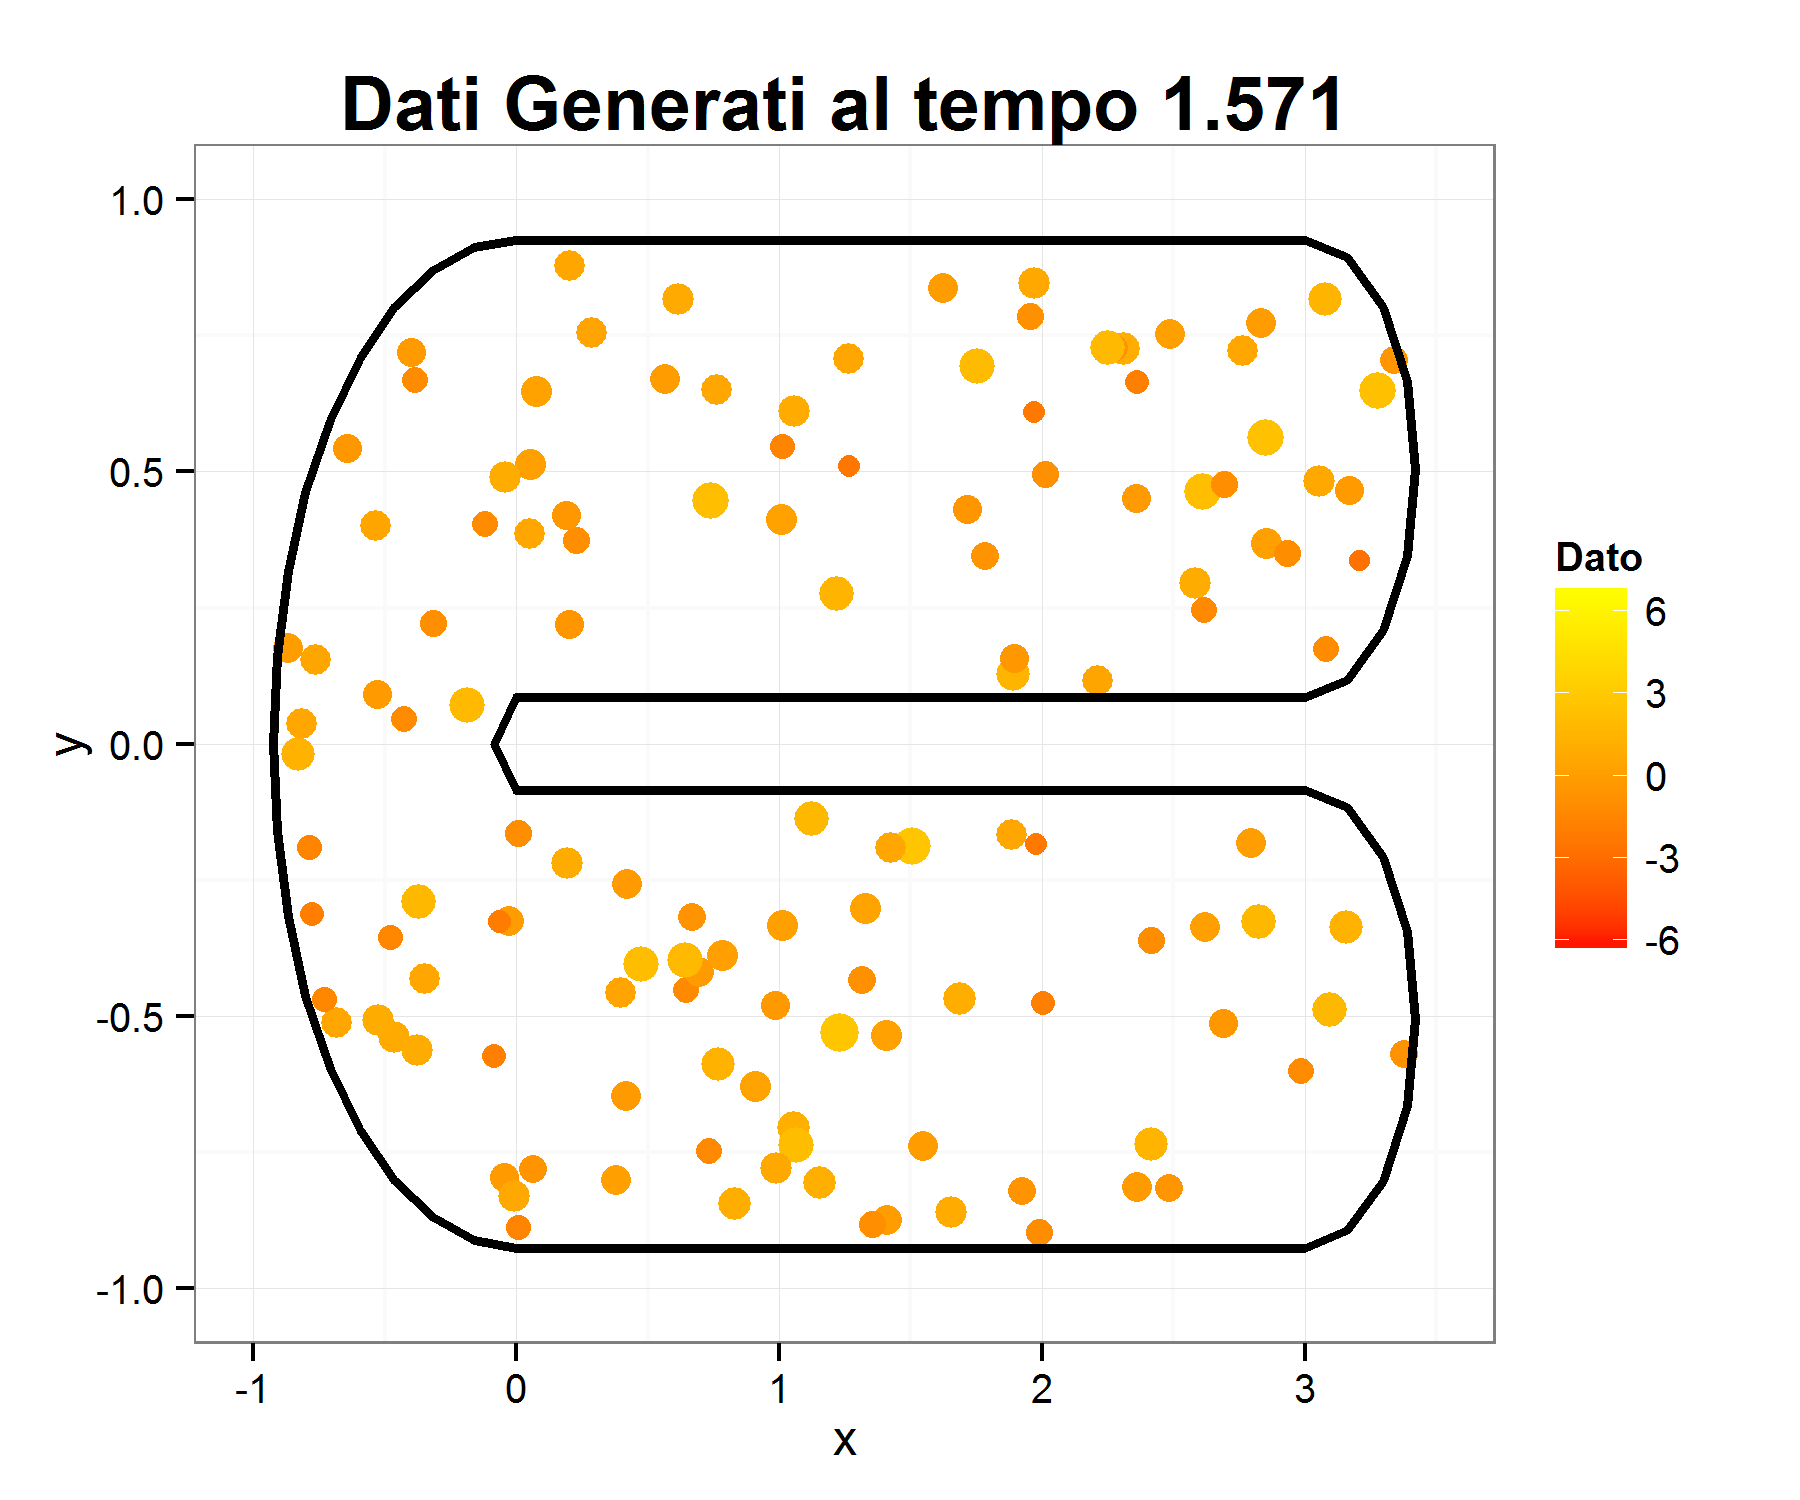
\includegraphics[height=0.25\textwidth]{immagini/simulazioni/Dati_tempo3.png}
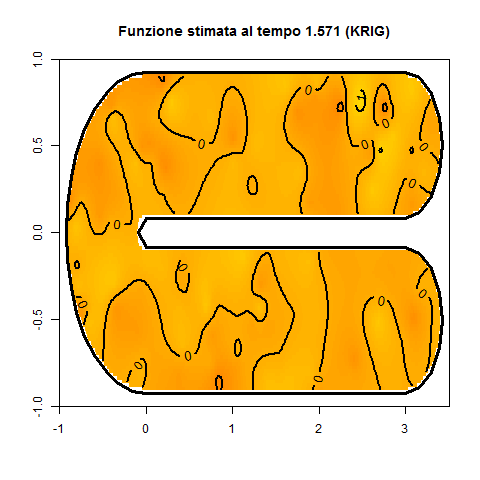
\includegraphics[width=0.25\textwidth]{immagini/simulazioni/KRIGtempo3.png}
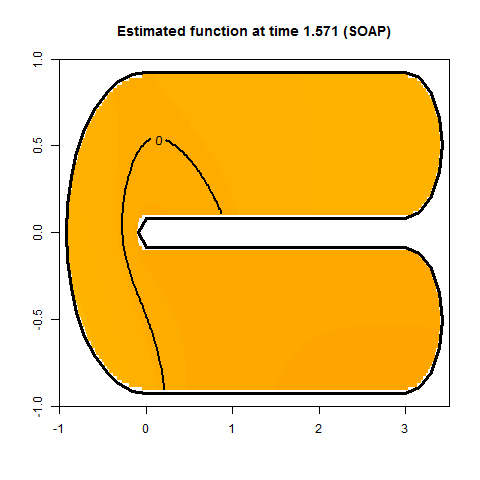
\includegraphics[width=0.25\textwidth]{immagini/simulazioni/SOAPtempo3.png}
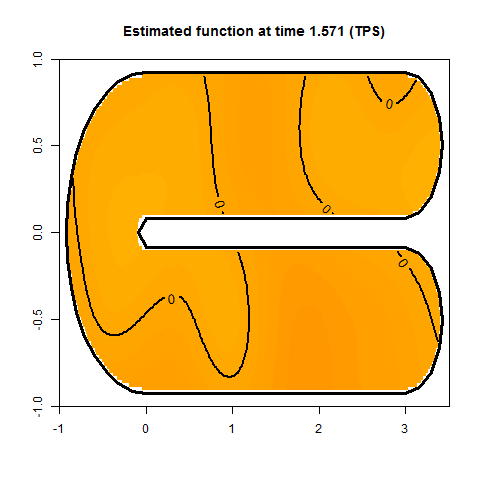
\includegraphics[width=0.25\textwidth]{immagini/simulazioni/TPStempo3.png}
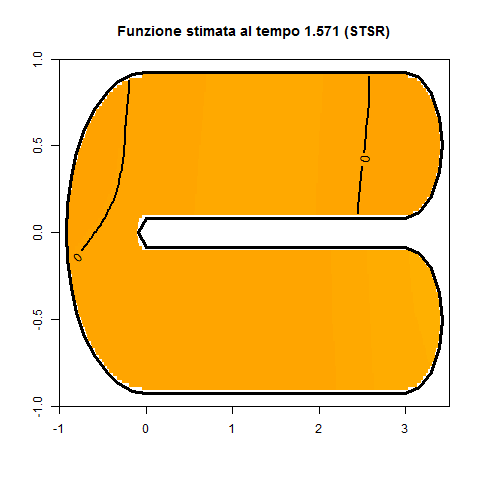
\includegraphics[width=0.25\textwidth]{immagini/simulazioni/STSRtempo3.png}

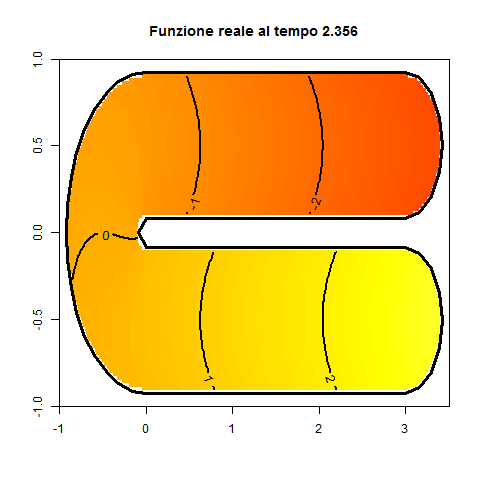
\includegraphics[width=0.25\textwidth]{immagini/simulazioni/REALEtempo4.png}
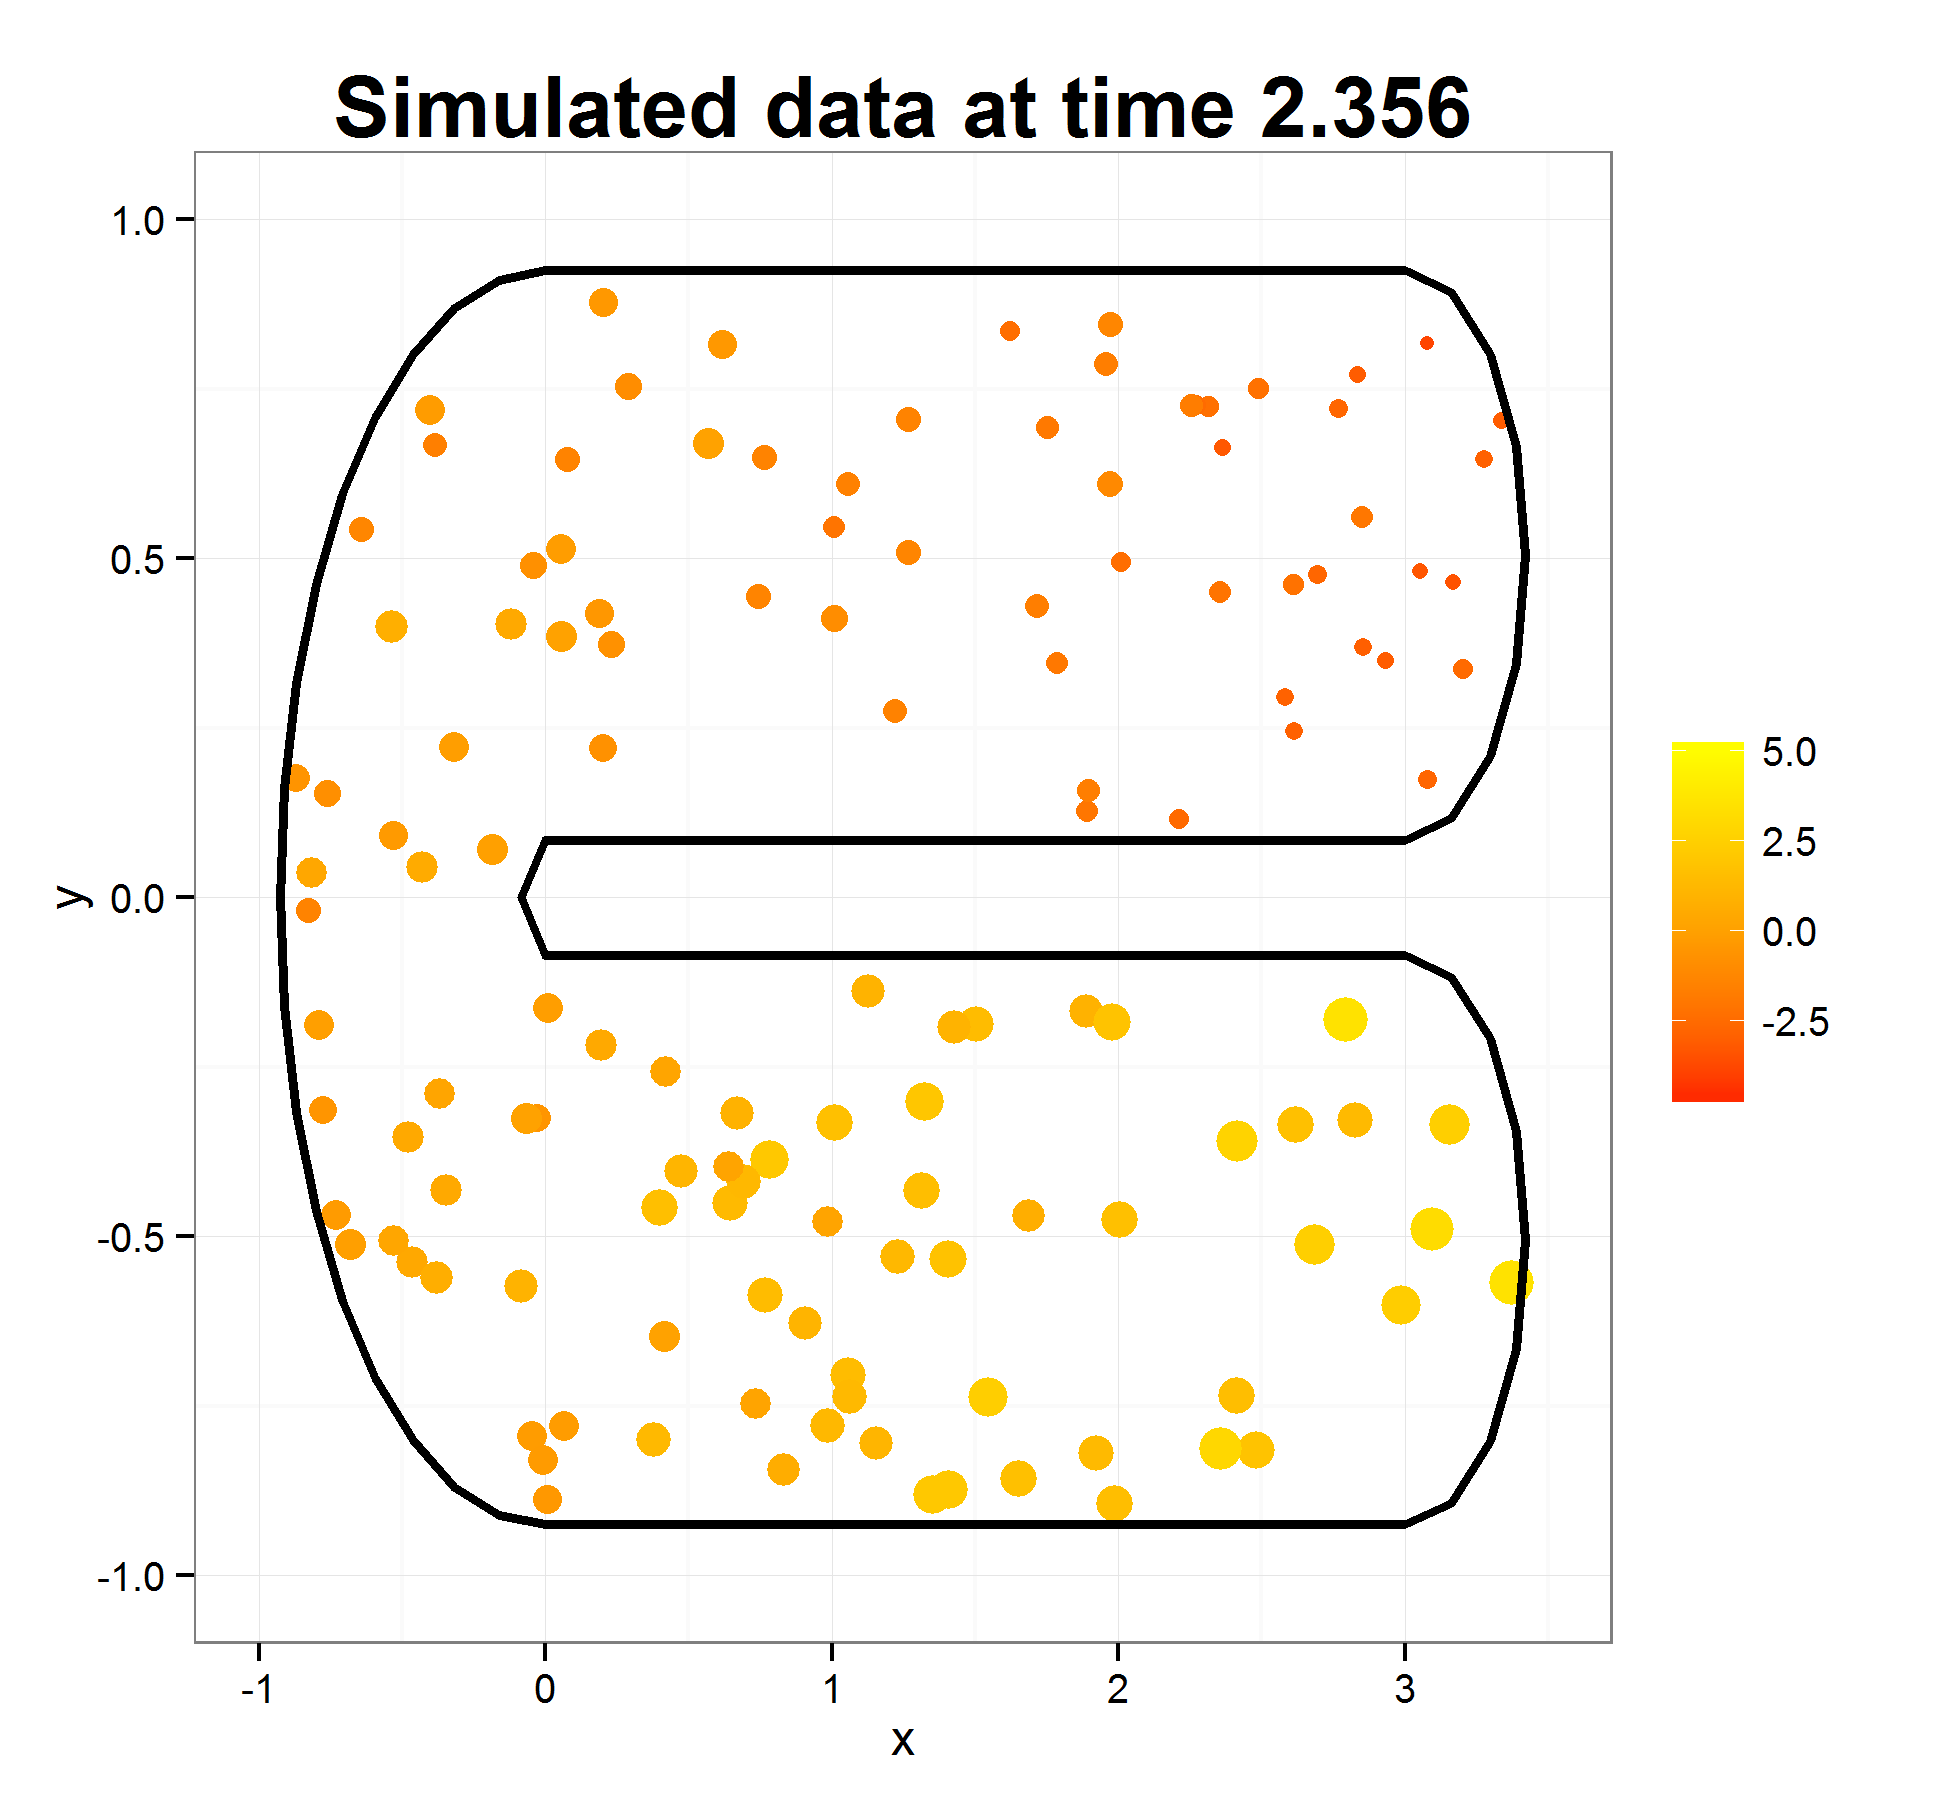
\includegraphics[height=0.25\textwidth]{immagini/simulazioni/Dati_tempo4.png}
\includegraphics[width=0.25\textwidth]{immagini/simulazioni/KRIGtempo4.png}
\includegraphics[width=0.25\textwidth]{immagini/simulazioni/SOAPtempo4.png}
\includegraphics[width=0.25\textwidth]{immagini/simulazioni/TPStempo4.png}
\includegraphics[width=0.25\textwidth]{immagini/simulazioni/STSRtempo4.png}

\caption{Per alcuni istanti di tempo, funzione test $f(\protect\underline{p},t)$ reale, dati simulati, stime ottenute rispettivamente con kriging spazio-temporale, GAMM con soap film smoothing, GAMM con thin plate splines e stima con STR-PDE nel caso senza covariata}
\label{fig:confronto_altri_metodi_nocov}
\end{figure}
\end{landscape}


\section{Caso con covariata}

La stessa analisi è stata eseguita nel caso con covariata. La covariata è stata generata in tutti i punti esattamente come fatto nel capitolo \ref{cap:domC}. Nella calcolo del RMSE è stato considerato solo il termine dipendente dalla funzione $f(\underline p,t)$, poiché non è opportuno generare nuovamente valori per la covariata nei punti di validazione. I boxplot riportati in fig. \ref{fig:cfrcovar1} possono quindi essere considerati come valutazione della bontà della stima della parte funzionale del modello. Per la parte spiegata dalla covariata sono stati tracciati i boxplot in fig. \ref{fig:cfrcovar2}, con le stime di $\hat{\beta}$ calcolate dai metodi. Il kriging, che nel caso senza covariata si è rivelato ampiamente peggiore degli altri metodi, non è stato considerato.

Le conclusioni sono perfettamente analoghe al caso precedente. La stima di $\beta$ non presenta differenze, ma nella parte funzionale il caso STR-PDE è nuovamente il migliore. Analogamente al caso senza covariata, dai plot della funzione stimata ad alcuni istanti di tempo fissati in fig. \ref{fig:confronto_altri_metodi_cov} si possono trarre le stesse conclusioni. Il modello STR-PDE è quello che più si avvicina alla funzione reale.

\begin{figure}[t]
	\centering
	\subfigure[$\mathrm{RMSE}$]
   {
   \label{fig:cfrcovar1}
	\includegraphics[width=0.46\textwidth]{Immagini/Confronto_metodi_covar.png}   
   }
	\subfigure[Stime $\protect\hat{\beta}$]
   {
   \label{fig:cfrcovar2}
	\includegraphics[width=0.46\textwidth]{Immagini/Confronto_metodi_beta.png}
   }
	\caption{Confronto tra i metodi, caso con covariata}
	\label{fig:cfrcovar}
\end{figure}

\begin{landscape}
\begin{figure}
\centering
\includegraphics[width=0.25\textwidth]{immagini/simulazioni_covar/REALEtempo1.png}
\includegraphics[height=0.25\textwidth]{immagini/simulazioni_covar/Dati_tempo1.png}
\includegraphics[width=0.25\textwidth]{immagini/simulazioni_covar/SOAPtempo1.png}
\includegraphics[width=0.25\textwidth]{immagini/simulazioni_covar/TPStempo1.png}
\includegraphics[width=0.25\textwidth]{immagini/simulazioni_covar/STSRtempo1.png}

\includegraphics[width=0.25\textwidth]{immagini/simulazioni_covar/REALEtempo2.png}
\includegraphics[height=0.25\textwidth]{immagini/simulazioni_covar/Dati_tempo2.png}
\includegraphics[width=0.25\textwidth]{immagini/simulazioni_covar/SOAPtempo2.png}
\includegraphics[width=0.25\textwidth]{immagini/simulazioni_covar/TPStempo2.png}
\includegraphics[width=0.25\textwidth]{immagini/simulazioni_covar/STSRtempo2.png}

\includegraphics[width=0.25\textwidth]{immagini/simulazioni_covar/REALEtempo3.png}
\includegraphics[height=0.25\textwidth]{immagini/simulazioni_covar/Dati_tempo3.png}
\includegraphics[width=0.25\textwidth]{immagini/simulazioni_covar/SOAPtempo3.png}
\includegraphics[width=0.25\textwidth]{immagini/simulazioni_covar/TPStempo3.png}
\includegraphics[width=0.25\textwidth]{immagini/simulazioni_covar/STSRtempo3.png}

\includegraphics[width=0.25\textwidth]{immagini/simulazioni_covar/REALEtempo4.png}
\includegraphics[height=0.25\textwidth]{immagini/simulazioni_covar/Dati_tempo4.png}
\includegraphics[width=0.25\textwidth]{immagini/simulazioni_covar/SOAPtempo4.png}
\includegraphics[width=0.25\textwidth]{immagini/simulazioni_covar/TPStempo4.png}
\includegraphics[width=0.25\textwidth]{immagini/simulazioni_covar/STSRtempo4.png}

\caption{Per alcuni istanti di tempo, funzione test $f(\protect\underline{p},t)$ reale, dati simulati, stime ottenute rispettivamente con GAMM con soap film smoothing, GAMM con thin plate splines e stima con STR-PDE nel caso con covariata}
\label{fig:confronto_altri_metodi_cov}
\end{figure}
\end{landscape}


\chapter{Analisi della produzione di rifiuti urbani nella provincia di Venezia}
\label{cap:rifiuti}

Come è già stato brevemente accennato in precedenza, l'applicazione scelta per il modello STR-PDE riguarda i dati della produzione di rifiuti urbani nel periodo di anni dal 1997 al 2011 nella provincia di Venezia. Per rifiuti urbani si intendono rifiuti domestici, rifiuti prodotti in locali, aree pubbliche, parchi, giardini o spiagge, rifiuti provenienti dalla pulizia delle strade o di altri luoghi pubblici. Non sono conteggiati i rifiuti speciali (tra cui ad esempio quelli industriali, agricoli o provenienti da attività commerciali o di costruzione) o pericolosi (per i quali esistono programmi di smaltimento particolari).

In realtà, come già precedentemente indicato, i dati raccolti dall'Agenzia Regionale per la Prevenzione e Protezione Ambientale del Veneto (Arpav) riguardano tutta la regione. Tuttavia è stata analizzata solo la provincia di Venezia per due motivi. Inanzitutto l'interesse particolare per la zona della laguna veneta, in cui è rilevante il ruolo del turismo (come si potrà notare in seguito). Inoltre considerare tutto il Veneto aumenterebbe notevolmente le dimensioni delle matrici in gioco causando una grossa spesa computazionale per la ricerca della soluzione. Quindi è stato scelto di concentrarsi su un dominio più piccolo ma nel quale è possibile notare più facilmente le particolarità dell'andamento del fenomeno della produzione dei rifiuti urbani.

Per ogni comune della provincia di Venezia e per ogni anno è disponibile il numero di rifiuti totali raccolti in tonnellate e la popolazione residente. La popolazione è certamente un valore influente per la produzione di rifiuti, perciò la quantità di riferimento non sarà il valore dei rifiuti totali raccolti in ogni anno per comune, ma il valore pro capite.

Le coordinate spaziali dei comuni sono la longitudine e la latitudine, disponibili on line\footnote{\href{http://www.dossier.net/utilities/coordinate-geografiche/}{http://www.dossier.net/utilities/coordinate-geografiche/}}. Nel caso dei comuni con dato replicato (sez \ref{sez:comunireplicati}), le coordinate sono state scaricate da Google Maps.


\section{L'inclusione dell'effetto del turismo}

L'inclusione della popolazione residente nella risposta tramite la scelta di usare i valori pro capite è necessaria, poiché permette di depurare la risposta da una variabile che per sua natura la influenzerebbe. Ma sarebbe un errore fermarsi solo alla popolazione residente, poiché anche i turisti rappresentano una componente non trascurabile di produzione di rifiuti urbani.

Nella provincia di Venezia sono presenti molte zone di elevata attrazione turistica. Grande importanza è da attribuire a Venezia, ma si hanno anche zone balneari (come Lido di Venezia, Cavallino-Treporti, Jesolo, San Michele al Tagliamento, Bibione, ecc...). L'informazione scelta per sintetizzare l'attività turistica è il numero di posti letto totali del comune, valore disponibile grazie all'applicativo dell'Istat \textit{Atlante Statistico dei Comuni}\footnote{\href{http://www.istat.it/it/archivio/113712}{http://www.istat.it/it/archivio/113712}} per ogni anno. Il totale dei posti letto per comune è la somma di vari tipi di attività non solamente alberghiere in senso stretto (ad esempio sono conteggiati anche esercizi complementari, bed \& breakfast, campeggi) e saranno considerati normalizzati per la popolazione residente per uniformità con la risposta. I valori ricavati saranno inseriti nel modello come possibile covariata.


\section{Trattamento del dominio}

Per poter studiare il problema a livello computazionale occorre avere una buona approssimazione della frontiera della regione. Questa è disponibile nel pacchetto R \textit{raster} che descrive dati geografici di moltissime zone del mondo sia a livello nazionale che locale (nel caso italiano province e comuni) tramite poligoni molto precisi.

Una volta scaricata la provincia di Venezia da \textit{raster}, si è riscontrato subito un problema: la regione è composta da un insieme di 101 poligoni distinti (a causa delle numerose isole di cui è composta la laguna) e ogni poligono ha un alto numero di vertici (ad esempio, la prima delle due regioni corrispondenti all'entroterra aveva 10538 vertici). Non è possibile analizzare il problema su un territorio così descritto, perciò è stata necessaria una analisi iniziale della frontiera per ridurne la complessità. 

\begin{figure}[t]
	\centering
	\subfigure[Tutti i poligoni]
   {
   \label{fig:Ven_poligonitutti}
	\includegraphics[width=0.46\textwidth]{Immagini/Ven_poligoni.png}   
   }
	\subfigure[Poligoni scelti]
   {
   \label{fig:Ven_poligoniscelti}
	\includegraphics[width=0.46\textwidth]{Immagini/Ven_poligoniscelti.png}
   }
	\caption{Poligoni disponibili nel pacchetto \textit{raster}}
	\label{fig:Ven_poligoni}
\end{figure}

Oltre all'entroterra (composto da due poligoni) stati scelte solo le più più rilevanti isole della laguna a livello di popolazione e turismo: Venezia, Murano, Lido di Venezia, Pellestrina e Chioggia (composta da due poligoni). In fig. \ref{fig:Ven_poligoni} (tracciata, come per le successive, con il pacchetto R \textit{RgoogleMaps}) sono visualizzati i poligoni disponibili e quelli scelti per l'analisi. Come sarà indicato nel paragrafo successivo, tutte queste isole sono state trattate per la riduzione dei vertici e, per creare un poligono unico, sono state unite tra loro con ponti dove era possibile. Tra le isole collegate solamente via mare con il resto del territorio sono stati simulati ponti in corrispondenza delle trafficate linee di trasporto pubblico con traghetto. 

\subsection{Regression splines}

Per ridurre l'elevato numero di vertici di ognuno dei poligoni considerati si è scelto di ricorrere ad un'analisi di smoothing di dati funzionali. Ad ogni poligono è associata una coppia di funzioni: la latitudine e la longitudine rispetto all'ascissa curvilinea (disponibili per punti, corrispondenti ai vertici di \textit{raster}) che sono state rappresentate in basi. Successivamente, le funzioni stimate sono state valutate in un mumero molto inferiore di punti, con i quali si è costruita la nuova definizione della regione.

Per avere una rappresentazione tramite funzioni di base di queste funzioni sono state provate più tecniche e la scelta definitiva è ricaduta sulle \textit{Regression Splines} cubiche senza penalizzazione della derivata seconda. Infatti i risultati non sono stati migliori con le altre tecniche provate a causa della zona interna alla laguna di Venezia, fortemente frastagliata: ad esempio penalizzare la derivata seconda eliminava troppe asperità presenti sulle coste del territorio, mentre con \textit{Kernel Smoothing} sono state ricavate regioni che, dopo la triangolazione, presentavano troppi triangoli composti solamente da punti di frontiera (e quindi senza dati) rispetto agli altri metodi.

Una volta fissato un ragionevole numero di punti con cui descrivere la regione sono stati eseguiti più tentativi per decidere il miglior numero di basi necessario per descrivere le due funzioni. Il criterio di scelta è stato complesso, poiché sono stati esclusi i valori che generavano intersezioni nella nuova descrizione della regione e comuni esterni alla frontiera. Ma la scelta del miglior numero di basi per \textit{Regression Splines} è ricaduta sul valore che, una volta eseguito lo smoothing della regione, causava la minor distanza tra i nuovi punti della regione e il poligono iniziale. In fig. \ref{fig:Ven_ent1} è riportato il risultato dello smoothing sul primo poligono che descrive l'entroterra della provincia di Venezia (nella versione definitiva ha 100 punti, molti meno dei 10538 iniziali).  

\begin{figure}[t]
	\centering
	\begin{minipage}{.32\textwidth}
	\includegraphics[width=\textwidth]{Immagini/Ven_Longitudine.png}
	\includegraphics[width=\textwidth]{Immagini/Ven_Latitudine.png}
	\end{minipage}%
	\begin{minipage}{.64\textwidth}
	\includegraphics[width=\textwidth]{Immagini/Ven_Regione.png}
	\end{minipage}
	\caption{Smoothing con \textit{Regression Splines} cubiche per il primo poligono dell'entroterra della provincia di Venezia}
	\label{fig:Ven_ent1}
\end{figure}

Dopo aver ripetuto l'analisi per ognuna delle isole elencate precedentemente (eccetto Chioggia, aggregata al dominio in modo molto più semplificato), la descrizione finale è stata ricavata unendo tra loro tutti i nuovi poligoni. In seguito è stata eliminata una zona costiera dell'entroterra della laguna di Venezia che, sebbene sia presente sia in \textit{raster} che nei grafici di Google Maps, corrisponde ad una parte fangosa e paludosa e quindi disabitata. Non essendo possibile che su di essa siano prodotti rifiuti è stata tagliata dalla regione. Per questo motivo si troverà sempre una zona non analizzata sui grafici con mappe da Google Maps. In fig. \ref{fig:Ven_rgm} è riportata la descrizione finale del dominio con i punti spaziali considerati (si consulti anche la sezione successiva).
\begin{figure}[t]
	\centering
	\subfigure[Provincia di Venezia]
   {
   \label{fig:Ven_rgm_tot}
	\includegraphics[width=0.46\textwidth]{Immagini/Ven_punti.png}   
   }
	\subfigure[Zoom della laguna]
   {
   \label{fig:Ven_rgm_zoom}
	\includegraphics[width=0.46\textwidth]{Immagini/Ven_puntizoom.png}
   }
	\caption{Frontiera e punti spaziali per la provincia di Venezia}
	\label{fig:Ven_rgm}
\end{figure}

\subsection{Scelte particolari tra i comuni}
\label{sez:comunireplicati}

L'uso di valori pro capite per rifiuti e posti letto consente di replicare il dato del comune anche su altri punti in cui risulta necessario. Ad esempio, le isole di Murano, Lido di Venezia e Pellestrina non sono sedi di comune, ma si riferiscono a Venezia. Quindi il dato di Venezia è stato replicato in queste isole ad ogni anno, per avere un valore di riferimento in quanto zone distaccate. Come si può notare in fig. \ref{fig:Ven_rgm_zoom} anche nell'isola di Venezia è stato duplicato il dato, per avere una triangolazione  senza troppi triangoli composti solo da punti di frontiera in una zona di particolare rilevanza.

Un caso particolare riguarda il comune di Cavallino-Treporti, che è stato istituito nel 1999 con una parte dei territori del comune di Venezia. La separazione all'interno dei dati, però, è presente dal 2002. Di conseguenza prima di questo anno il dato in Cavallino-Treporti è una replica del dato di Venezia.

\subsection{Triangolazione del dominio}

La triangolazione è stata prodotta tramite il pacchetto R \textit{RTriangle}. Poiché nella zona ad est il numero di capoluoghi di comune (e quindi di nodi della triangolazione) è minore rispetto al resto della regione, è stata fissata un'area massima per i triangoli generati da \textit{RTriangle}. Questo ha reso la triangolazione più fitta anche dove non lo sarebbe stata, e garantirà una stima della risposta più precisa nella zona balneare che, come si potrà notare in seguito, ha una grande importanza per la distribuzione dei rifiuti. Affinchè questo sia possibile sono stati aggiuhnti nuovi punti spaziali, che restano senza dato per tutta l'analisi. In fig. \ref{fig:Ven_triang} si ha la triangolazione finale che sarà usata da ora in avanti.

\begin{figure}[t]
\centering
\subfigure[Provincia di Venezia]
   {
   \label{fig:Ven_triang_tot}
	\includegraphics[width=0.46\textwidth]{Immagini/Ven_triang.png}   
   }
\subfigure[Zoom della laguna]
   {
   \label{fig:Ven_triang_zoom}
	\includegraphics[width=0.46\textwidth]{Immagini/Ven_triangzoom.png}
   }
\caption{Triangolazione della provincia di Venezia}
\label{fig:Ven_triang}
\end{figure}

In conclusione, il dominio è descritto da 414 punti (41 con dati, 373 di frontiera o aggiunti dalla triangolazione) e da 475 triangoli.

\section{Analisi preliminare dei dati}
Prima di eseguire l'analisi, è opportuno avere una visualizzazione dei dati sul dominio della provincia di Venezia. In fig. \ref{fig:Ven_bubbledati} sono riportati i bubbleplot dei dati (realizzati grazie all'aiuto del paccherro R \textit{ggmap}), che permettono di avere un'idea del fenomeno in spazio e tempo.
\newpage
\begin{figure}[H]
	\centering
	\includegraphics[trim=0cm 0cm 0cm 0cm,clip=true,width=0.45\textwidth]{Immagini/venezia_dati/Dati1997.png}
	%\includegraphics[trim=0cm 0cm 0cm 2cm,clip=true,width=0.45\textwidth]{Immagini/venezia_dati/Dati1998.png}
	\includegraphics[trim=0cm 0cm 0cm 0cm,clip=true,width=0.45\textwidth]{Immagini/venezia_dati/Dati1999.png}
	%\includegraphics[trim=0cm 0cm 0cm 2cm,clip=true,width=0.45\textwidth]{Immagini/venezia_dati/Dati2000.png}
	\includegraphics[trim=0cm 0cm 0cm 0cm,clip=true,width=0.45\textwidth]{Immagini/venezia_dati/Dati2001.png}
	%\includegraphics[trim=0cm 0cm 0cm 2cm,clip=true,width=0.45\textwidth]{Immagini/venezia_dati/Dati2002.png}
	\includegraphics[trim=0cm 0cm 0cm 0cm,clip=true,width=0.45\textwidth]{Immagini/venezia_dati/Dati2003.png}
	%\includegraphics[trim=0cm 0cm 0cm 2cm,clip=true,width=0.45\textwidth]{Immagini/venezia_dati/Dati2004.png}
	\includegraphics[trim=0cm 0cm 0cm 0cm,clip=true,width=0.45\textwidth]{Immagini/venezia_dati/Dati2005.png}
	%\includegraphics[trim=0cm 0cm 0cm 2cm,clip=true,width=0.45\textwidth]{Immagini/venezia_dati/Dati2006.png}
	\includegraphics[trim=0cm 0cm 0cm 0cm,clip=true,width=0.45\textwidth]{Immagini/venezia_dati/Dati2007.png}
	%\includegraphics[trim=0cm 0cm 0cm 2cm,clip=true,width=0.45\textwidth]{Immagini/venezia_dati/Dati2008.png}
	\includegraphics[trim=0cm 0cm 0cm 0cm,clip=true,width=0.45\textwidth]{Immagini/venezia_dati/Dati2009.png}
	%\includegraphics[trim=0cm 0cm 0cm 2cm,clip=true,width=0.45\textwidth]{Immagini/venezia_dati/Dati2010.png}
	\includegraphics[trim=0cm 0cm 0cm 0cm,clip=true,width=0.45\textwidth]{Immagini/venezia_dati/Dati2011.png}
	\caption{Bubbleplot delle misurazioni della produzione di rifiuti urbani pro capite ogni due anni dal 1997 al 2011}
	\label{fig:Ven_bubbledati}
\end{figure}
\newpage
\begin{figure}[H]
	\centering
	\includegraphics[trim=0cm 0cm 0cm 0cm,clip=true,width=0.45\textwidth]{Immagini/venezia_dati/PL1997.png}
	%\includegraphics[trim=0cm 0cm 0cm 2cm,clip=true,width=0.45\textwidth]{Immagini/venezia_dati/PL1998.png}
	\includegraphics[trim=0cm 0cm 0cm 0cm,clip=true,width=0.45\textwidth]{Immagini/venezia_dati/PL1999.png}
	%\includegraphics[trim=0cm 0cm 0cm 2cm,clip=true,width=0.45\textwidth]{Immagini/venezia_dati/PL2000.png}
	\includegraphics[trim=0cm 0cm 0cm 0cm,clip=true,width=0.45\textwidth]{Immagini/venezia_dati/PL2001.png}
	%\includegraphics[trim=0cm 0cm 0cm 2cm,clip=true,width=0.45\textwidth]{Immagini/venezia_dati/PL2002.png}
	\includegraphics[trim=0cm 0cm 0cm 0cm,clip=true,width=0.45\textwidth]{Immagini/venezia_dati/PL2003.png}
	%\includegraphics[trim=0cm 0cm 0cm 2cm,clip=true,width=0.45\textwidth]{Immagini/venezia_dati/PL2004.png}
	\includegraphics[trim=0cm 0cm 0cm 0cm,clip=true,width=0.45\textwidth]{Immagini/venezia_dati/PL2005.png}
	%\includegraphics[trim=0cm 0cm 0cm 2cm,clip=true,width=0.45\textwidth]{Immagini/venezia_dati/PL2006.png}
	\includegraphics[trim=0cm 0cm 0cm 0cm,clip=true,width=0.45\textwidth]{Immagini/venezia_dati/PL2007.png}
	%\includegraphics[trim=0cm 0cm 0cm 2cm,clip=true,width=0.45\textwidth]{Immagini/venezia_dati/PL2008.png}
	\includegraphics[trim=0cm 0cm 0cm 0cm,clip=true,width=0.45\textwidth]{Immagini/venezia_dati/PL2009.png}
	%\includegraphics[trim=0cm 0cm 0cm 2cm,clip=true,width=0.45\textwidth]{Immagini/venezia_dati/PL2010.png}
	\includegraphics[trim=0cm 0cm 0cm 0cm,clip=true,width=0.45\textwidth]{Immagini/venezia_dati/PL2011.png}
	\caption{Bubbleplot dei posti letto pro capite ogni due anni dal 1997 al 2011}
	\label{fig:Ven_bubblePL}
\end{figure}
\newpage
\begin{figure}[t]
\centering
	\includegraphics[width=0.60\textwidth]{Immagini/Matplot.png}   
 \caption{Matplot della produzione dei rifiuti urbani}
   \label{fig:Ven_matplot}
\end{figure}
Da questa analisi iniziale si può già notare come la produzione di rifiuti sia più alta nella zona balneare della regione e che non abbia grosse variazioni nel tempo, poiché i dati sono più o meno simili negli anni. Questo è evidenziato anche in fig. \ref{fig:Ven_matplot}, dove i dati risultano raggruppabili in due gruppi (zona balneare e altri comuni) totalmente distinti, eccetto per un comune (Cavallino-Treporti) che subisce un forte innalzamento nel tempo.

Gli stessi grafici sono stati ripetuti in fig. \ref{fig:Ven_bubblePL} per il numero di posti letto pro capite. Il numero di posti letto assume valori decisamente più alti nella zona balneare rispetto al resto della regione. Contrariamente a quello che ci si aspettava, non si hanno molto posti letto nell'isola di Venezia. Invece si ha una grossa variazione nel comune di Cavallino-Treporti dopo la separazione dal comune di Venezia (si nota che il raggio della bolla aumenta notevolmente dopo il 2002). Questo indica che i posti letto sono in realtà numerosi in Cavallino-Treporti, ma quando era unito al comune di Venezia questo effetto non poteva essere colto in modo così dettagliato. Ci si può quindi aspettare che la funzione stimata presenti un comportamento differente in Cavallino-Treporti nelle due situazioni.

\subsection{Funzioni di base}
Le basi in spazio scelte per l'applicazione del modello sono gli elementi finiti lineari anche in questo caso. Ad ognuno dei punti spaziali (interni o di frontiera) è associata una funzione di base, coerentemente con la triangolazione prodotta. Di conseguenza si ha $N=414$ mentre il numero di punti con dati $n$ è minore ed è pari a 41.

In tempo, esattamente come nel caso del dominio a forma di C, sono state scelte come funzioni di base le B-splines cubiche. L'intervallo temporale per la descrizione del dominio è $[1997,2011]$ e i dati sono disponibili con cadenza annuale. Anche in questo caso si assume che il numero di basi sia pari al numero di istanti temporali a disposizione, quindi $M=m=15$.

\section{Applicazione del modello senza covariata}

\subsection{Ricerca del miglior $\protect\underline{\lambda}$}

Prima di calcolare i risultati dell'analisi occorre fissare i parametri $\lambda_S$ e $\lambda_T$. Il procedimento è perfettamente analogo a quello ricavato nel caso del dominio a forma di C, minimizzando la quantità $\mathrm{GCV}(\underline \lambda)$ in eq. \ref{eq:GCV}. In tab. \ref{tab:Ven} sono disponibili i risultati.
\newline
\begin{table}[h]
\renewcommand{\arraystretch}{1.3}
\setlength{\tabcolsep}{2mm}
\centering
	\begin{tabular}{!{\vrule width 1.2pt}c!{\vrule width 1.2pt}c!{\vrule width 1.2pt}}
	\noalign{\hrule height 1.2pt}
	Intervalli per $\log_{10}\lambda_S$ e $\log_{10}\lambda_T$& Miglior valore											\\
	\noalign{\hrule height 1.2pt}
	$\log_{10}\lambda_S \in \{-12,-11,\ldots,+1\}$ 	& \multirow{2}{*}{$\underline \lambda = (10^{-10},10^{0})$} 			\\
	\cline{1-1}
	$\log_{10}\lambda_T \in \{-8,-7,\ldots,+1\}$		& 															\\	
	\noalign{\hrule height 1.2pt}
	$\log_{10}\lambda_S \in \{-11,-10.5,\ldots,-9\}$ 	& \multirow{2}{*}{$\underline \lambda = (10^{-9.5},10^{0})$} 		\\
	\cline{1-1}
	$\log_{10}\lambda_T \in \{-1,-0.5,\ldots,+1\}$	& 															\\	
	\noalign{\hrule height 1.2pt}
	$\log_{10}\lambda_S \in \{-10,-9.875,\ldots,-9\}$ 	& \multirow{2}{*}{$\underline \lambda = (10^{-9.625}, 10^{0})$}	\\
	\cline{1-1}
	$\log_{10}\lambda_T \in \{-0.5,-0.375,\ldots,+0.5\}$		& 			\\	
	\noalign{\hrule height 1.2pt}
	\end{tabular}
\caption{Analisi di $\mathrm{GCV}(\protect\underline{\lambda})$ per la provincia di Venezia, caso senza covariata}
\label{tab:Ven}
\end{table}

\subsection{Risultati}
La produzione dei rifiuti è stata analizzata con $\underline \lambda = (10^{-9.625}, 10^{0})$. In fig. \ref{fig:Ven_ris} sono riportati i risultati ottenuti nei 15 anni a disposizione. Questi grafici (grazie anche alla visualizzazione sulle mappe di Google Maps) permettono di studiare il profilo della funzione nei vari istanti temporali e di avere un'idea dell'evoluzione della produzione di rifiuti a livello geografico.
\newpage
\begin{figure}[H]
\centering
	\includegraphics[trim=0cm 0cm 4cm 0cm,clip=true,width=0.32\textwidth]{Immagini/venezia_senza_covariate/Maps1997.png}
	\includegraphics[trim=0cm 0cm 4cm 0cm,clip=true,width=0.32\textwidth]{Immagini/venezia_senza_covariate/Maps1998.png}
	\includegraphics[trim=0cm 0cm 4cm 0cm,clip=true,width=0.32\textwidth]{Immagini/venezia_senza_covariate/Maps1999.png}
	\includegraphics[trim=0cm 0cm 4cm 0cm,clip=true,width=0.32\textwidth]{Immagini/venezia_senza_covariate/Maps2000.png}
	\includegraphics[trim=0cm 0cm 4cm 0cm,clip=true,width=0.32\textwidth]{Immagini/venezia_senza_covariate/Maps2001.png}
	\includegraphics[trim=0cm 0cm 4cm 0cm,clip=true,width=0.32\textwidth]{Immagini/venezia_senza_covariate/Maps2002.png}
	\includegraphics[trim=0cm 0cm 4cm 0cm,clip=true,width=0.32\textwidth]{Immagini/venezia_senza_covariate/Maps2003.png}
	\includegraphics[trim=0cm 0cm 4cm 0cm,clip=true,width=0.32\textwidth]{Immagini/venezia_senza_covariate/Maps2004.png}
	\includegraphics[trim=0cm 0cm 4cm 0cm,clip=true,width=0.32\textwidth]{Immagini/venezia_senza_covariate/Maps2005.png}
	\includegraphics[trim=0cm 0cm 4cm 0cm,clip=true,width=0.32\textwidth]{Immagini/venezia_senza_covariate/Maps2006.png}
	\includegraphics[trim=0cm 0cm 4cm 0cm,clip=true,width=0.32\textwidth]{Immagini/venezia_senza_covariate/Maps2007.png}
	\includegraphics[trim=0cm 0cm 4cm 0cm,clip=true,width=0.32\textwidth]{Immagini/venezia_senza_covariate/Maps2008.png}
	\includegraphics[trim=0cm 0cm 4cm 0cm,clip=true,width=0.32\textwidth]{Immagini/venezia_senza_covariate/Maps2009.png}
	\includegraphics[trim=0cm 0cm 4cm 0cm,clip=true,width=0.32\textwidth]{Immagini/venezia_senza_covariate/Maps2010.png}
	\includegraphics[trim=0cm 0cm 4cm 0cm,clip=true,width=0.32\textwidth]{Immagini/venezia_senza_covariate/Maps2011.png}
	\caption{Stima della funzione spazio-temporale della produzione dei rifiuti nella provincia di Venezia a tempi fissati dal 1997 al 2011, caso senza covariata}
	\label{fig:Ven_ris}
\end{figure}
\newpage
Come si può notare dai grafici, ci sono due zone ad elevato valore di produzione dei rifiuti pro capite, corrispondenti a località con grande interesse turistico per le spiagge presenti. Ad est, tra le altre, si hanno le località turistiche di Bibione (confinante con Lignano Sabbiadoro, che però è oltre il confine) e Caorle. Scendendo verso sud-ovest si nota che anche Jesolo causa un innalzamento della funzione che descrive la risposta. La produzione dei rifiuti è particolarmente alta in queste zone turistiche e, contrariamente a ciò che si poteva immaginare, molto più di Venezia. Quindi, come già si notava dai bubbleplot in fig. \ref{fig:Ven_bubblePL}, il turismo sarà rilevante nell'analisi della produzione di rifiuti, e la causa non sarà Venezia (dove la produzione non è eccessivamente diversa dagli altri comuni) ma saranno le località balneari.

\begin{figure}[t]
	\centering
	\subfigure[Venezia]
   {
	\includegraphics[width=0.31\textwidth]{Immagini/venezia_senza_covariate/Venezia.png}   
   }
	\subfigure[Cavallino-Treporti]
   {
	\includegraphics[width=0.31\textwidth]{Immagini/venezia_senza_covariate/Cavallino-Treporti.png}
   }
	\subfigure[Chioggia]
   {
	\includegraphics[width=0.31\textwidth]{Immagini/venezia_senza_covariate/Chioggia.png}   
   }
	\subfigure[Jesolo]
   {
	\includegraphics[width=0.31\textwidth]{Immagini/venezia_senza_covariate/Jesolo.png}
   }
	\subfigure[Caorle]
   {
	\includegraphics[width=0.31\textwidth]{Immagini/venezia_senza_covariate/Caorle.png}   
   }
	\subfigure[S. Michele al Tagliamento]
   {
	\includegraphics[width=0.31\textwidth]{Immagini/venezia_senza_covariate/SanMichelealTagliamento.png}
   }
	\caption{Stima della produzione dei rifiuti pro capite in alcuni comuni, caso senza covariata}
	\label{fig:Ven_tempo}
\end{figure}

In fig. \ref{fig:Ven_tempo} sono tracciati gli sviluppi temporali stimati in alcuni comuni. I punti rossi corrispondono al dato misurato. La funzione stimata spiega bene l'andamento tracciato dai dati iniziali senza cadere nell'eccessiva interpolazione. Infatti lo smoothing imposto dal modello tramite la penalizzazione della derivata seconda in tempo permette di non avere variazioni repentine. Ad esempio, nei grafici di Venezia e Cavallino-Treporti, il cambio di andamento dovuto alla separazione del comune dal 2002 ha provocato un cambiamento ma è stato comunque colto dal modello. Si noti come la risposta cresca velocemente in Cavallino-Treporti (come già notato in \ref{fig:Ven_matplot}). In Chioggia e in Jesolo si ha un calo generale della produzione dei rifiuti, mentre in San Michele al Tagliamento (comune di appartenenza di Bibione) e Caorle si hanno valori alti, a conferma dei grafici in \ref{fig:Ven_ris}.

\subsection{Analisi dei residui}

\begin{figure}[t]
	\centering
	\subfigure[$z_{ij}$ vs $e_{ij}$]
	{
	\includegraphics[width=0.46\textwidth]{Immagini/venezia_senza_covariate/Scatterplot1.png}  
   }
	\subfigure[$\hat{z}_{ij}$ vs $e_{ij}$]
   {
	\includegraphics[width=0.46\textwidth]{Immagini/venezia_senza_covariate/Scatterplot2.png}
   }
	\caption{Scatterplot dei residui, caso senza covariata}
	\label{fig:Ven_residui}
\end{figure}
Contrariamente a quanto fatto in precedenza nel caso di dominio a forma di C, non si può prescindere dall'analisi dei residui per verificare l'ipotesi di omogeneità in varianza. Tramite gli scatterplot in fig. \ref{fig:Ven_residui} si può concludere che l'ipotesi è rispettata poiché i residui si dispongono come una nuvola uniformemente distribuita intorno allo zero.


\section{Applicazione del modello con covariata}

\subsection{Ricerca del miglior $\protect\underline{\lambda}$}
Prima di eseguire l'analisi, come al solito, occorre cercare buoni valori per $\underline \lambda$. Dalla tab. \ref{tab:Vencovar} si possono seguire le iterazioni eseguite e il risultato finale.
\newpage
\begin{table}[h]
\renewcommand{\arraystretch}{1.3}
\setlength{\tabcolsep}{2mm}
\centering
	\begin{tabular}{!{\vrule width 1.2pt}c!{\vrule width 1.2pt}c!{\vrule width 1.2pt}}
	\noalign{\hrule height 1.2pt}
	Intervalli per $\log_{10}\lambda_S$ e $\log_{10}\lambda_T$& Miglior valore											\\
	\noalign{\hrule height 1.2pt}
	$\log_{10}\lambda_S \in \{-12,-11,\ldots,+1\}$ 	& \multirow{2}{*}{$\underline \lambda = (10^{-8},10^{0})$} 			\\
	\cline{1-1}
	$\log_{10}\lambda_T \in \{-8,-7,\ldots,+1\}$		& 															\\	
	\noalign{\hrule height 1.2pt}
	$\log_{10}\lambda_S \in \{-9,-8.5,\ldots,-7\}$ 	& \multirow{2}{*}{$\underline \lambda = (10^{-8},10^{0})$} 		\\
	\cline{1-1}
	$\log_{10}\lambda_T \in \{-1,-0.5,\ldots,+1\}$	& 															\\	
	\noalign{\hrule height 1.2pt}
	$\log_{10}\lambda_S \in \{-8.5,-8.375,\ldots,-7.5\}$ 	& \multirow{2}{*}{$\underline \lambda = (10^{-7.750}, 10^{-0.125})$}	\\
	\cline{1-1}
	$\log_{10}\lambda_T \in \{-0.5,-0.375,\ldots,+0.5\}$		& 			\\	
	\noalign{\hrule height 1.2pt}
	\end{tabular}
\caption{Analisi di $\mathrm{GCV}(\protect\underline{\lambda})$ per la provincia di Venezia, caso con covariata}
\label{tab:Vencovar}
\end{table}

\subsection{Risultati}
Le analisi sono state eseguite con $\underline \lambda = (10^{-7.750}, 10^{-0.125})$. Come si può notare dai grafici in fig. \ref{fig:Vencovar_ris}, dove è riportata la stima della funzione $f(\underline p,t)$ in tutti i punti senza l'aggiunta della parte spiegata dalla covariata, nelle zone dove la produzione di rifiuti è massima si hanno ora i valori più bassi.
\newpage
\begin{figure}[H]
\centering
\includegraphics[trim=0cm 0cm 4cm 0cm,clip=true,width=0.32\textwidth]{Immagini/venezia_con_covariate/Maps1997.png}
\includegraphics[trim=0cm 0cm 4cm 0cm,clip=true,width=0.32\textwidth]{Immagini/venezia_con_covariate/Maps1998.png}
\includegraphics[trim=0cm 0cm 4cm 0cm,clip=true,width=0.32\textwidth]{Immagini/venezia_con_covariate/Maps1999.png}
\includegraphics[trim=0cm 0cm 4cm 0cm,clip=true,width=0.32\textwidth]{Immagini/venezia_con_covariate/Maps2000.png}
\includegraphics[trim=0cm 0cm 4cm 0cm,clip=true,width=0.32\textwidth]{Immagini/venezia_con_covariate/Maps2001.png}
\includegraphics[trim=0cm 0cm 4cm 0cm,clip=true,width=0.32\textwidth]{Immagini/venezia_con_covariate/Maps2002.png}
\includegraphics[trim=0cm 0cm 4cm 0cm,clip=true,width=0.32\textwidth]{Immagini/venezia_con_covariate/Maps2003.png}
\includegraphics[trim=0cm 0cm 4cm 0cm,clip=true,width=0.32\textwidth]{Immagini/venezia_con_covariate/Maps2004.png}
\includegraphics[trim=0cm 0cm 4cm 0cm,clip=true,width=0.32\textwidth]{Immagini/venezia_con_covariate/Maps2005.png}
\includegraphics[trim=0cm 0cm 4cm 0cm,clip=true,width=0.32\textwidth]{Immagini/venezia_con_covariate/Maps2006.png}
\includegraphics[trim=0cm 0cm 4cm 0cm,clip=true,width=0.32\textwidth]{Immagini/venezia_con_covariate/Maps2007.png}
\includegraphics[trim=0cm 0cm 4cm 0cm,clip=true,width=0.32\textwidth]{Immagini/venezia_con_covariate/Maps2008.png}
\includegraphics[trim=0cm 0cm 4cm 0cm,clip=true,width=0.32\textwidth]{Immagini/venezia_con_covariate/Maps2009.png}
\includegraphics[trim=0cm 0cm 4cm 0cm,clip=true,width=0.32\textwidth]{Immagini/venezia_con_covariate/Maps2010.png}
\includegraphics[trim=0cm 0cm 4cm 0cm,clip=true,width=0.32\textwidth]{Immagini/venezia_con_covariate/Maps2011.png}
\caption{Stima della funzione spazio-temporale della produzione dei rifiuti nella provincia di Venezia a tempi fissati dal 1997 al 2011, con covariata}
\label{fig:Vencovar_ris}
\end{figure}

\begin{figure}[t]
	\centering
	\subfigure[Venezia]
   {
	\includegraphics[width=0.31\textwidth]{Immagini/venezia_con_covariate/Venezia.png}   
   }
	\subfigure[Cavallino-Treporti]
   {
	\includegraphics[width=0.31\textwidth]{Immagini/venezia_con_covariate/Cavallino-Treporti.png}
   }
	\subfigure[Chioggia]
   {
	\includegraphics[width=0.31\textwidth]{Immagini/venezia_con_covariate/Chioggia.png}   
   }
	\subfigure[Jesolo]
   {
	\includegraphics[width=0.31\textwidth]{Immagini/venezia_con_covariate/Jesolo.png}
   }
	\subfigure[Caorle]
   {
	\includegraphics[width=0.31\textwidth]{Immagini/venezia_con_covariate/Caorle.png}   
   }
	\subfigure[S. Michele al Tagliamento]
   {
	\includegraphics[width=0.31\textwidth]{Immagini/venezia_con_covariate/SanMichelealTagliamento.png}
   }
	\caption{Stima della parte funzionale della produzione dei rifiuti pro capite in alcuni comuni, con covariata}
	\label{fig:Vencovar_tempo}
\end{figure}
\newpage
In fig. \ref{fig:Vencovar_tempo} si hanno anche i grafici della funzione stimata (senza il termine di covariata) in alcuni comuni. I punti tracciati in rosso rappresentano il dato, a cui è sottratta la covariata moltiplicata per $\hat{\beta}$ stimato. Non possono essere considerati come la parte di dati generati esattamente dalla funzione, ma come una loro buona approssimazione (ma sono comunque ciò che è riconosciuto dal modello per la stime di $\hat{\underline{c}}$, come già evidenziato in sez. \ref{sez:beta}).

L'interpretazione del risultato in questo caso è legata all'alta affluenza turistica nelle zone balneari. Come si può notare dai grafici iniziali dalle fig. \ref{fig:Ven_bubbledati} e \ref{fig:Ven_bubblePL}, su tutta la zona costiera non si hanno solo i massimi dei rifiuti pro capite ma anche del numero di posti letto pro capite. Quindi non soltanto la produzione di rifiuti è massima nella zona balneare (come già si notava dalla funzione stimata nel caso senza covariata) ma anche l'attività turistica. In questo caso
$$
\hat{\beta}\approx284.05 \ .
$$
Più la covariata è alta, più è sottratta informazione alla funzione $f(\underline p,t)$ poiché $\hat{\beta}$ è costante in spazio e tempo. Perciò la funzione ha un profilo quasi simile ad una traslazione del caso senza covariate nel resto del dominio (in questa zona il numero di posti letto pro capite, come si nota in fig. \ref{fig:Ven_bubblePL}, è quasi costante) e ribassato nella zona balneare, a causa dell'alto contributo della covariata.

Interessante è quanto accade nel comune di Cavallino-Treporti, dove la funzione subisce una grossa variazione dopo la divisione dal comune di Venezia per l'aumento del numero dei posti letto. Attorno all'anno 2002 si ha uno stravolgimento dell'andamento della funzione. Tuttavia, essendo dovuto alla maggior precisione del dato in Cavallino-Treporti, è un cambiamento utile a spiegar meglio la risposta. Gli effetti dovuti alle propiretà di smoothing poste dal modello sono analoghi al caso senza covariata, si ha una spiegazione dell'andamento generale della funzione senza cogliere troppo il dato e senza interpolare. Nelle località dove si avevano i valori massimi nel caso senza covariata, ora si hanno i minimi a causa dei posti letto (in alcuni casi la funzione è addirittura negativa).

\subsection{Analisi dei residui}

\begin{figure}[t]
	\centering
	\subfigure[$z_{ij}$ vs $e_{ij}$]
	{
	\includegraphics[width=0.46\textwidth]{Immagini/venezia_con_covariate/Scatterplot2.png}  
	}
	\subfigure[$\hat{z}_{ij}$ vs $e_{ij}$]
   {
	\includegraphics[width=0.46\textwidth]{Immagini/venezia_con_covariate/Scatterplot3.png}
   }
	\caption{Scatterplot dei residui, caso con covariata}
	\label{fig:Vencovar_residui}
\end{figure}
Anche in questo caso è necessario controllare l'ipotesi di omoschedasticità dei residui. I risultati sono perfettamente analoghi al caso senza covariata e si può concludere che l'ipotesi è rispettata.
\newpage
\begin{figure}[h]
	\centering
	\includegraphics[width=0.45\textwidth]{Immagini/venezia_con_covariate/QQplot.png}   
   \caption{QQplot dei residui, caso con covariata}
	\label{fig:Ven_qqplot}
\end{figure}
Essendo presente una covariata, potrebbe essere interessante calcolare per essa intervalli di confidenza o verificare alcune ipotesi. Pertanto in questo caso è opportuno controllare anche l'eventuale gaussianità dei residui. Dal QQplot in fig. \ref{fig:Ven_qqplot}, troppo distante da una retta, e dal p-value del Shapiro-Wilk test, che è stimato minore di $2\times 10^{-16}$, si deduce che la gaussianità non può essere ipotizzata e quindi non è possibile calcolare intervalli di confidenza come fatto per il dominio a forma di C.





\chapter{Conclusioni e sviluppi futuri}
\label{cap:conclusione}

In questo lavoro di tesi è stato analizzato nel dettaglio il modello STR-PDE nell'ambito della stima funzionale per dati varianti all'interno di un dominio spaziale e di un intervallo temporale. Il modello, che si propone di essere un'estensione del caso puramente spaziale già analizzato in letteratura, è stato sviluppato in codice R. Dal confronto con gli altri metodi e da quanto ricavato con le stime, soprattutto sul dominio a forma di C in cui è possibile conoscere il valore reale della funzione, si può concludere che i risultati prodotti sono molto buoni.

Diversa è la conclusione per le prestazioni computazionali del codice. Per semplicità computazionale le basi degli elementi finiti sono state scelte lineari e la produzione dei rifiuti è stata analizzata solamente nella provincia di Venezia, pur avendo a disposizione i dati di tutto il Veneto. Inoltre, durante l'esecuzione del codice, si è potuto notare come alcune funzioni come la minimizzazione di $\mathrm{GCV}(\underline \lambda)$ o il calcolo dei valori stimati ad un istante di tempo fissato (usati ad esempio per conoscere il profilo della funzione ad un certo anno) siano molto lente. Ovviamente per analisi di dataset di grosse dimensioni deve essere messa in conto una spesa di tempo elevata, ma R certamente non ha aiutato. Infatti, è noto che R non sia un linguaggio di programmazione fortemente efficiente, e questo ha caratterizzato la lentezza di esecuzione. Il più chiaro sviluppo futuro può essere l'uso del codice come base per la creazione di un algoritmo più veloce attraverso l'integrazione con un linguaggio di programmazione più efficiente (come il C++) o dell'eventuale parallelizzazione nei colli di bottiglia più evidenti.

Dopo che sarà stata sviluppata l'integrazione del codice sarà possibile garantire una analisi più agile anche per dataset di dimensioni più elevate o per elementi finiti di ordine maggiore. In questo modo si avrà a disposizione uno strumento di analisi statistica buono non solo dal punto di vista dei risultati, ma anche in termini di efficienza computazionale.


\begin{thebibliography}{99}

\bibitem{art:augustin}
Nicole H. Augustin, Verena M. Trenkel, Simon N. Wood, Pascal Lorance, \emph{Space-time modelling of blue ling for fisheries stock management}, Environmetrics, 24, 109–119, (2013)

\bibitem{art:azzimonti}
Laura Azzimonti, Laura M. Sangalli, Piercesare Secchi, Maurizio Domanin, Fabio Nobile, \emph{Blood flow velocity field estimation via spatial regression with PDE penalization}, Journal of the American Statistical Association, (2015)

\bibitem{art:gcv}
Peter Craven, Grace Wahba, \emph{Smoothing noisy data with spline functions: estimating the correct degree of smoothing by the method of generalized cross-validation}, Numerische Mathematik, 31, 377–403, (1979)

\bibitem{art:marra}
Giampiero Marra, David L. Miller, Luca Zanin, \emph{Modelling the spatiotemporal distribution of the incidence of resident foreign population}, Statistica Neerlandica, 66, 133–160, (2012)

\bibitem{art:ramsay}
Timothy O. Ramsay, \emph{Spline smoothing over difficult regions}, Journal of the Royal Statistical Society: Series B, 64, 307–319, (2002)

\bibitem{art:sangalli}
Laura M. Sangalli, James O. Ramsay, Timothy O. Ramsay, \emph{Spatial spline regression models}, Journal of the Royal Statistical Society: Series B, 75, 681–703, (2013)

\bibitem{art:wood}
Simon N. Wood, Mark W. Bravington, Sharon L. Hedley, \emph{Soap film smoothing}, Journal of the Royal Statistical Society: Series B, 70, 931–955, (2008)

\bibitem{prog:R}
R Core Team, \emph{R: A Language and Environment for Statistical Computing}, R Foundation for Statistical Computing, Vienna, 2013, \href{http://www.R-project.org/}{http://www.R-project.org/}


\bibitem{package:fda}
J. O. Ramsay, Hadley Wickham, Spencer Graves and Giles Hooker (2014). \emph{fda: Functional Data Analysis}. R package version 2.4.3. \href{http://CRAN.R-project.org/package=fda}{http://CRAN.R-project.org/package=fda}

\bibitem{package:Matrix}
Douglas Bates and Martin Maechler (2015). \emph{Matrix: Sparse and Dense Matrix Classes and Methods}. R package version 1.1-5. \href{http://CRAN.R-project.org/package=Matrix}{http://CRAN.R-project.org/package=Matrix}

\bibitem{package:RTriangle}
Shewchuk JR (1996). \emph{Triangle: Engineering a 2D quality mesh generator and Delaunay triangulator}. In Lin MC and Manocha D (eds.), Applied Computational Geometry: Towards Geometric Engineering, volume 1148 series Lecture Notes in Computer Science, pp. 203-222. Springer-Verlag. From the First ACM Workshop on Applied Computational Geometry.

\bibitem{package:mgcv1}
Wood, S.N. (2011) \emph{Fast stable restricted maximum likelihood and marginal likelihood estimation of semiparametric generalized linear models}. Journal of the Royal Statistical Society (B) 73(1):3-36

\bibitem{package:mgcv2}
Wood, S.N. (2004) \emph{Stable and efficient multiple smoothing parameter estimation for generalized additive models}. Journal of the American Statistical Association. 99:673-686.

\bibitem{package:mgcv3}
Wood, S.N. (2006) \emph{Generalized Additive Models: An Introduction with R}. Chapman and Hall/CRC.

\bibitem{package:mgcv4}
Wood, S.N. (2003) \emph{Thin-plate regression splines}. Journal of the Royal Statistical Society (B) 65(1):95-114.
  
\bibitem{package:mgcv5}
Wood, S.N. (2000) \emph{Modelling and smoothing parameter estimation with multiple quadratic penalties}. Journal of the Royal Statistical Society (B) 62(2):413-428.

\bibitem{package:gstat}
Pebesma, E.J., 2004. \emph{Multivariable geostatistics in S: the gstat package}. Computers \& Geosciences, 30: 683-691.

\bibitem{package:raster}
Robert J. Hijmans (2015). \emph{raster: Geographic data analysis and modeling}. R package version 2.3-24. \href{http://CRAN.R-project.org/package=raster}{http://CRAN.R-project.org/package=raster}

\bibitem{package:rgooglemaps}
Markus Loecher (2014). \emph{RgoogleMaps: Overlays on Google map tiles in R}. R package version 1.2.0.6. \href{http://CRAN.R-project.org/package=RgoogleMaps}{http://CRAN.R-project.org/package=RgoogleMaps}
  
\bibitem{package:loa1}
Karl Ropkins (2014). \emph{loa: various plots, options and add-ins for use with lattice}. R package version 0.2.15.

\bibitem{package:loa2}
Karl Ropkins, David C. Carslaw, Said Munir and Haibo Chen (2012). \emph{R, lattice and RgoogleMaps: A practical framework for the development of new geovisualizations}. Invited paper for Special Session on Statistical Graphics, American Statistical Association (ASA) 2012 Joint Statistical Meeting, San Diego, US, 29 July - 2 August, 2012.

\bibitem{package:ggplot2}
H. Wickham. \emph{ggplot2: elegant graphics for data analysis}. Springer New York, 2009.

\bibitem{package:ggmap}
D. Kahle and H. Wickham. \emph{ggmap: Spatial Visualization with ggplot2}. The R Journal, 5(1), 144-161. \href{http://journal.r-project.org/archive/2013-1/kahle-wickham.pdf}{http://journal.r-project.org/archive/2013-1/kahle-wickham.pdf}

\end{thebibliography}


\end{document}
